\documentclass[a4paper]{article}
\usepackage{fullpage} % Package to use full page 
\usepackage{tikz} % Package for drawing
\usepackage{pgfplots}
\usepackage{amsmath}
\usepackage{physics}
\usepackage{multirow} 

\usepackage{caption}
\usepackage{subcaption}

\usepackage{siunitx} %% units
\usepackage[inline]{enumitem}%%%%% enumerate setting
\usepackage{hyperref}
% \usepackage{nopageno} %%% if no page number needed 

\usepackage{aircraftshapes} %%% helicopter draw by github source

%\usepackage{wrapfig} %% wrap figures
\usepackage{rotating}  %% table  symbol rotate 

\usetikzlibrary{decorations.pathmorphing, patterns,arrows} %%% draw springs
	
\usetikzlibrary{shapes.geometric} %% draw ellipse

\usetikzlibrary{trees} %% draw tree diagram
\usetikzlibrary{calc}  %%% sqrt calculation

\usepackage{amssymb}

\setlength{\parindent}{0pt} %%% global setting for paragraph indent.

\newcounter{Exercise}  %%% define the Exercise number %% put [section] after {Exercise} if needed
\newcommand\exercise{\vspace{1cm}\par\noindent\stepcounter{Exercise} \textbf{Exercise}  \theExercise} %% define the default Exercise style

\newcounter{Miscellaneous}  %%% define the Miscellaneous exercise number %% put [section] after {Exercise} if needed
\newcommand\mis{\vspace{1cm}\par\noindent\stepcounter{Miscellaneous} \textbf{Miscellaneous exercise}  \theMiscellaneous} %% define the default Miscellaneous Exercise style

\newcounter{Examstyle}  %%% define the Exam style exercise number %% put [section] after {Exercise} if needed
\newcommand\exam{\vspace{1cm}\par\noindent\stepcounter{Examstyle} \textbf{Exam-style Questions}  \theExamstyle} %% define the default Miscellaneous Exercise style


\renewcommand{\familydefault}{\sfdefault} %% sans font as a default 
 

\let\tempone\itemize  %% change the default itemize space
\let\temptwo\enditemize
\renewenvironment{itemize}{\tempone\addtolength{\itemsep}{2\baselineskip}}{\temptwo}


\pgfplotsset{my style/.append style={axis lines=center,
		xmajorticks=true, 	 
		ymajorticks=true,
		xlabel={$x$},
		ylabel={$y$},
		x label style={=at={(current axis.right of origin), anchor=north},right =2mm},	
		y label style={=at={(current axis.up of origin), anchor=north},above=1mm}}}
%% default setting for x-y plane
 
\begin{document}
	\section{Representation of data}
%%%%%%%%%%%%%%%%%%%%%%%%%%%%%%%%%%%%%%%%%%%%%
%%%%%%%%%%%%%%%%%%%%%%%%%%%%%%%%%%%%%%%%%%%%%
%%%%%%%%%%%%%%%%%%%%%%%%%%%%%%%%%%%%%%%%%%%%%
%%%%%%%%%%%%%%%%%%%%%%%%%%%%%%%%%%%%%%%%%%%%%
%% 1.1 Terminologies %%%
%%%%%%%%%%%%%%%%%%%%%%%%%%%%%%%%%%%%%%%%%%%%%
%%%%%%%%%%%%%%%%%%%%%%%%%%%%%%%%%%%%%%%%%%%%%
%%%%%%%%%%%%%%%%%%%%%%%%%%%%%%%%%%%%%%%%%%%%%
%%%%%%%%%%%%%%%%%%%%%%%%%%%%%%%%%%%%%%%%%%%%%
\subsection{Terminologies}

Note the following terms:

\begin{itemize}

	\item qualitative data
	
	
	$\underline{\hspace{3cm}}$ or $\underline{\hspace{3cm}}$  are often used to show the information.
	\item quantitative data (numerical values)
	
	There are two types:  $\underline{\hspace{3cm}}$ and $\underline{\hspace{3cm}}$.
	
	
	\item frequency distribution
	
	Case $1$:
	\vspace{1cm}
	
	Case $2$:
	
	
	\item class boundry, interval width
	
\end{itemize}






\exercise  %% Exercise 1

\begin{enumerate}  %%% P1 example 1.1
	\item  The table shows the areas of different categories of land use in a particular region.
	\medskip
	
	\renewcommand{\arraystretch}{1.2} % default is 1.0
	\begin{tabular}{|c|c|c|c|c|c|}
		\hline
		Category &  Urban & Woodland & Farmland & Reservoris & Total \\ 
		\hline
		Area($\si{\km\squared}$) & 615 & 660 & 1200 & 225 & 2700 \\ 
		\hline
	\end{tabular}

\smallskip

Illustrate the data diagramatically.

\item  In a survey on the number of letters in the solutions of a crossword puzzle, the following data were obtained from the crossword puzzle in Monday's newspapaer.

\begin{tabular}{cccccccccc}
	\rule[-1ex]{0pt}{2.5ex} 9 & 5 & 7 & 7 & 5 & 12 & 6 & 6 & 12 & 5 \\
	\rule[-1ex]{0pt}{2.5ex} 7 & 7 & 5 & 5 & 3 & 7 & 3 & 7 & 9 & 6 \\
	\rule[-1ex]{0pt}{2.5ex} 3 & 5 & 7 & 3 & 6 & 7 & 7 & 6 & 3 & 7 \\
\end{tabular}

Draw a frequency distribution table for the data.



\item  The following data were obtained in a survey of heights of 20 children in a sports club. Each height was measured to the nearest centimetre.

\begin{tabular}{cccccccccc}
	\rule[-1ex]{0pt}{2.5ex} 133 & 136 & 120 & 138 & 133 & 131 & 127 & 141 & 127 & 143 \\
	\rule[-1ex]{0pt}{2.5ex} 130 & 131 & 125 & 144 & 128 & 134 & 135 & 137 & 133 & 129 \\
\end{tabular}

Draw a frequency distribution table for the data.
\end{enumerate}


\newpage


%%%%%%%%%%%%%%%%%%%%%%%%%%%%%%%%%%%%%%%%%%%%%
%%%%%%%%%%%%%%%%%%%%%%%%%%%%%%%%%%%%%%%%%%%%%
%%%%%%%%%%%%%%%%%%%%%%%%%%%%%%%%%%%%%%%%%%%%%
%%%%%%%%%%%%%%%%%%%%%%%%%%%%%%%%%%%%%%%%%%%%%
%% 1.2 Stem and leaf diagram %%%
%%%%%%%%%%%%%%%%%%%%%%%%%%%%%%%%%%%%%%%%%%%%%
%%%%%%%%%%%%%%%%%%%%%%%%%%%%%%%%%%%%%%%%%%%%%
%%%%%%%%%%%%%%%%%%%%%%%%%%%%%%%%%%%%%%%%%%%%%
%%%%%%%%%%%%%%%%%%%%%%%%%%%%%%%%%%%%%%%%%%%%%
\subsection{Stem-and-leaf diagram}

A way of grouping data into intervals while still retaining  the original data is to draw a \textbf{stem-and-leaf diagram}. 

\vspace{5 pt}


For example, there are 20 students in an assignment, their marks are as follows:
\vspace{5 pt}

\begin{tabular}{cccccccccc}
	\rule[-1ex]{0pt}{2.5ex} 84 & 17 & 38 & 45 & 47 & 53 & 76 & 54 & 75 & 32 \\
	\rule[-1ex]{0pt}{2.5ex} 66 & 65 & 55 & 54 & 51 & 44 & 39 & 19 & 54 & 72 \\
\end{tabular}

\vspace{5 pt}
A final plot of stem-and-leaf diagram would be like: 

\begin{table}[htbp]
	\centering
	

	
	\begin{tabular}{c|l@{\hspace{4 pt}}l@{\hspace{4 pt}}l@{\hspace{4 pt}}l@{\hspace{4 pt}}l@{\hspace{4 pt}}l@{\hspace{4 pt}} 	c}
		
		Stem & Leaf  & \\ 
		1     & 7 9 & (2)\\    
		2     &  & (0)\\    
		3     & 2 8 9 & (3)\\    
		4     & 4 5 7 & (3)\\    
		5     & 1 3 4 4 4 5 & (6)\\    
		6     & 5 6 & (2)\\
		7     & 2 5 6 & (3)\\
		8     & 4 &(1) \\
		
		
	\end{tabular}
\vspace{4 pt}

\fbox{ Key: $1 | 1 $ means 17 marks}

     \caption{Stem-and-leaf diagram of assignment marks}
	\label{tab:addlabel}
	
\end{table}

\textbf{Important}: You must always give a $\underline{\hspace{2 cm}}$ to explain what the stem and leaf  represent.
\medskip

 Also, $\underline{\hspace{4 cm}}$ must be chosen in a stem-and-leaf diagram.

\bigskip

For two sets of data, $\underline{\hspace{6 cm}}$ is often used to compare the data.


\exercise %% Exercise 2

\begin{enumerate} %% 
	\item  The lengths, in metres, of 20 measurements in a physics experiments are recorded as follows.
	\vspace{5 pt}
	
	\begin{tabular}{cccccccccc}
		\rule[-1ex]{0pt}{2.5ex} 1.78 & 1.87 & 1.89 & 1.72 & 1.68 & 2.04 & 1.96 & 1.76 & 1.90 & 1.73 \\
		\rule[-1ex]{0pt}{2.5ex} 1.78 & 1.61 & 1.78 & 1.77 & 1.85 & 1.65 & 1.89 & 1.95 & 2.01 & 1.83 \\
	\end{tabular}
\begin{enumerate}
	\item Represent this information on a stem-and-leaf diagram.
	\item State the mode.
\end{enumerate}
 


\item The maximum temperature in $\si{\celsius}$, measured to the nearest degree, was recorded each day during June in a particular city. The temperature were as follows:

\begin{tabular}{ccccccccccccccc}
	\rule[-1ex]{0pt}{2.5ex} 19 & 23 & 19 & 19 & 20 & 12 & 19 & 22 & 22 & 16 & 18 & 16 & 19 & 20 & 17 \\
	\rule[-1ex]{0pt}{2.5ex} 13 & 14 & 12 & 15 & 17 & 16 & 17 & 19 & 22 & 22 & 20 & 19 & 19 & 20 & 20 \\
\end{tabular}

Draw a stem-and-leaf diagram to illustrate the temperatures and write down the mode.


\item These are the examination marks for French and for English achieved by pupils in a particular class.

\begin{tabular}{ccccccccccc}
	\rule[-1ex]{0pt}{2.5ex} French & 43 & 55 & 29 & 49 & 36 & 55 & 61 & 34 & 42 & 42 \\
	\rule[-1ex]{0pt}{2.5ex}    & 54 & 60 & 48 & 23 & 44 & 31 & 55 & 45 & 37 & 57 \\
	\rule[-1ex]{0pt}{2.5ex} English & 80 & 65 & 74 & 59 & 79 & 92 & 52 & 71 & 43 & 86 \\
	\rule[-1ex]{0pt}{2.5ex}    & 60 & 74 & 57 & 41 & 79 & 74 & 58 & 52 & 64 & 84 \\
\end{tabular}

Draw a back-to-back stem-and-leaf diagram to compare the two sets of marks.
	
\end{enumerate}









%%%%%%%%%%%%%%%%%%%%%%%%%%%%%%%%%%%%%%%%%%%%%
%%%%%%%%%%%%%%%%%%%%%%%%%%%%%%%%%%%%%%%%%%%%%
%%%%%%%%%%%%%%%%%%%%%%%%%%%%%%%%%%%%%%%%%%%%%
%%%%%%%%%%%%%%%%%%%%%%%%%%%%%%%%%%%%%%%%%%%%%
%% 1.3 Histogram %%%
%%%%%%%%%%%%%%%%%%%%%%%%%%%%%%%%%%%%%%%%%%%%%
%%%%%%%%%%%%%%%%%%%%%%%%%%%%%%%%%%%%%%%%%%%%%
%%%%%%%%%%%%%%%%%%%%%%%%%%%%%%%%%%%%%%%%%%%%%
%%%%%%%%%%%%%%%%%%%%%%%%%%%%%%%%%%%%%%%%%%%%%

\newpage 

\subsection{Histograms}

Grouped data can be displayed in a \textbf{histogram}, as in the following diagram:
\vspace{0.5cm}

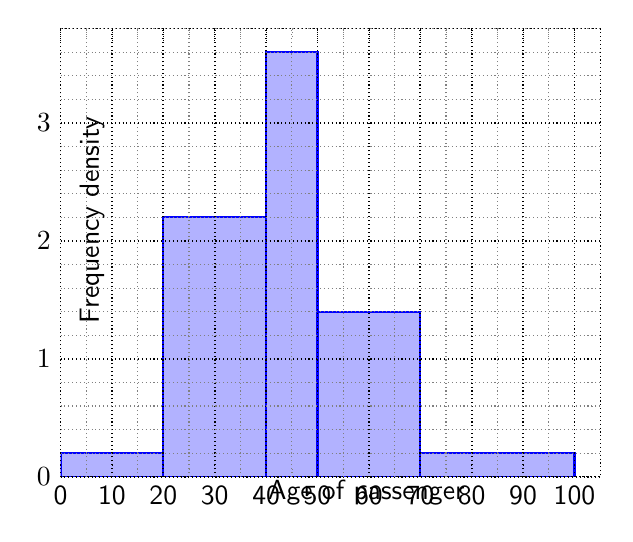
\begin{tikzpicture}
\centering

\begin{axis}[
area style,
densely dotted,
grid = both,
minor grid style=gray,
major grid style =black,
major grid style ={line width =0.6pt},
%	major grid style =thick,
major tick style=black,	
xmin = 0, xmax=105,
ymin=0, ymax= 3.8,
grid = both,
minor y tick num=4,
minor x tick num=1,
xtick={0,10,20,30,40,50,60,70,80,90,100},
xticklabels={0,10,20,30,40,50,60,70,80,90,100},	
x label style={at={(current axis.right of origin)},anchor=north, below=2mm, left =16mm},
y label style={at={(current axis.above origin)},anchor = west, below =4mm,left = 10mm},
xlabel={Age of passenger},
ylabel={Frequency density}
]


\addplot+[ybar interval,mark=no,thick,solid] plot coordinates { 
	(0,.2)
	(20,2.2)
	(40,3.6)
	(50,1.4)
	(70,0.2)
	(100,.2)
	
};


\end{axis}
\end{tikzpicture}

The frequency distribution table would be like:
\vspace{0.5cm}

\renewcommand{\arraystretch}{1.2} % default is 1.0
\begin{tabular}{|c|c|c|c|c|c|}
	\hline
	Age, $x$ years & $0 \leqslant x < 20$  & $20 \leqslant x < 40$ & $40 \leqslant x < 50$ & $50 \leqslant x < 70$ & $70 \leqslant x < 100$ \\
	\hline
	Frequency &  &  &  &  &  \\
	\hline
\end{tabular}

\bigskip

Notice the difference between histogram and $\underline{\hspace{2 cm}}$:

\begin{itemize}
	\setlength\itemsep{4em}
	\item 
	\item 
\end{itemize}

\bigskip

Frequency density:

\[
\text{frequency density} = \frac{\text{\qquad \qquad frequency \qquad \qquad  }}{}.
\]

\vspace{1cm}

Modal class: the interval with the greatest $\underline{\hspace{4 cm}}$.

\vspace{0.5cm}

Gaps treatment:

\begin{itemize}
	\setlength\itemsep{4em}
	\item Gropued continuous data (rounded values)
	\item Grouped discrete data (continuity correction, "0"): 
\end{itemize}
\vspace{0.5cm}





\newpage

The shape of a distribution:

\medskip
\vspace{6cm}

Positive skew  \hspace{4.2cm} Symmetrical  \hspace{4.2cm} \hfill Negative skew



 \exercise  %% Exercise 3

\begin{enumerate}
	\item A survey on the duration of telephone calls made to an office on a particular day gave the following results.
	
	\medskip
	
	%\renewcommand{\arraystretch}{1.2} % default is 1.0
	\begin{tabular}{|c|c|c|c|c|}
		\hline
		Duration, $t$ minutes & $1 \leqslant t < 3$  & $3 \leqslant t < 9$ & $9 \leqslant t < 15$ & $15 \leqslant t < 20$  \\
		\hline
		Frequency & 10 & 42 & 12 & 7   \\
		\hline
	\end{tabular}
\smallskip

     Draw a histogram to represent the data.
     
     \item The grouped frequency table records the weights, to the nearest gram, of the letters delievered to an apartment block on a particular day.
     
     	\medskip
     
     %\renewcommand{\arraystretch}{1.2} % default is 1.0
     \begin{tabular}{|c|c|c|c|c|c|}
     	\hline
     	Weight (gram) & $31-50$  & $51-60$ & $61-70$ & $71-100$ & $101-150$ \\
     	\hline
     	Frequency & 16 & 25 & 36 & 33 & 10   \\
     	\hline
     \end{tabular}
 \smallskip
 
 Draw a histogram to represent the data and state the modal class.
 
 \item $\dagger$ One evening a waiter measured the amounts of water left by diners in the bottles on the table in a restaurant. The volume were measured to the nearest millimetre.
 
 	\medskip
 
 %\renewcommand{\arraystretch}{1.2} % default is 1.0
 \begin{tabular}{|c|c|c|c|c|}
 	\hline
 	Volume (nearest \si{\ml}) & $0-19$  & $20-39$ & $40-89$ & $90-189$  \\
 	\hline
 	Frequency & 10 & 8 & 12 & 20   \\
 	\hline
 \end{tabular}
 \smallskip
 
  Draw a histogram to represent the data and state the modal class.
  
  \item These are marks in a statistics test for a group of 120 A level students.
  	\medskip
  
  %\renewcommand{\arraystretch}{1.2} % default is 1.0
  \begin{tabular}{|c|c|c|c|c|c|}
  	\hline
  	Mark & $0-9 $  & $10-19$ & $20-29$ & $30-49$ & $50-79$ \\
  	\hline
  	Frequency & 8 & 21 & 53 & 28 & 10   \\
  	\hline
  \end{tabular}
  \smallskip
  
  Draw a histogram to represent the data.
  \newpage 
  \item A Passenger's Association conducted a survey on the lateness of trains arriving at a particular railway station. The results are illustrated in the histogram.  
  \vspace{0.5cm}
  
  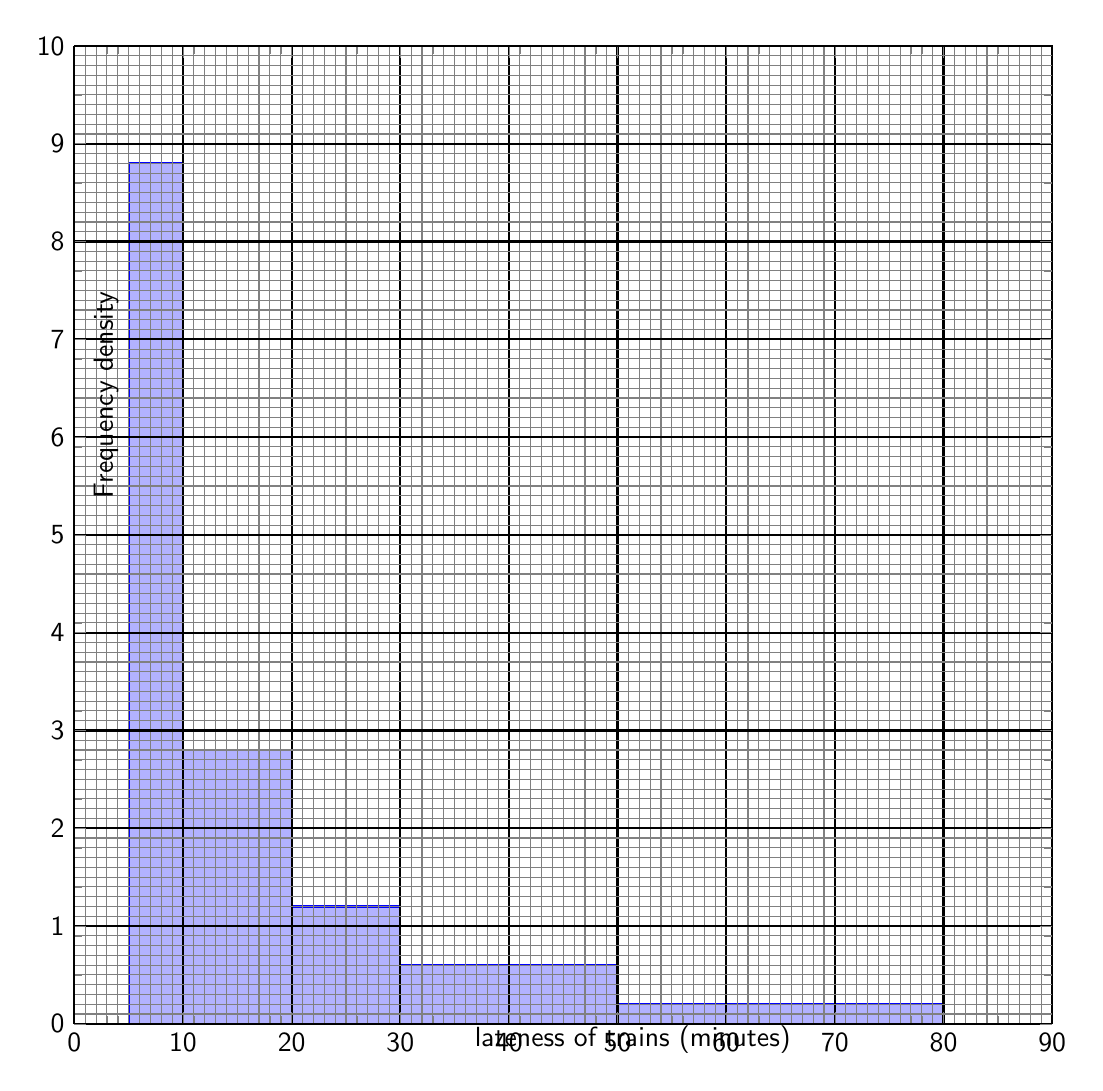
\begin{tikzpicture}
  \centering
  
  \begin{axis}[
  	width=14cm,
  	height=14cm,
  area style,
  solid,
  grid = both,
  minor grid style=gray,
  major grid style =black,
  major grid style ={line width =0.8pt},
  xmin = 0, xmax=90,
  ymin=0, ymax= 10,  
  minor y tick num=9,
  minor x tick num=9, 
  xtick={0,10,20,30,40,50,60,70,80,90},
  xticklabels={0,10,20,30,40,50,60,70,80,90},
  ytick={0,1,2,3,4,5,6,7,8,9,10},
  yticklabels={0,1,2,3,4,5,6,7,8,9,10}, 
  x label style={at={(current axis.right of origin)},anchor=north, below=2mm, left =32mm},
  y label style={at={(current axis.above origin)},anchor = west, below =4mm,left = 30mm},
  xlabel={lateness of trains (minutes)},
  ylabel={Frequency density}
  ]
  
  
  \addplot+[ybar interval,mark=no,thick,solid] plot coordinates { 
  	(0,6.4)
  	
  	(5,8.8)
  	(10,2.8)
  	(20,1.2)
  	(30,0.6)
  	(50,0.2)
  	(80,0)
  	
  };
  
  
  \end{axis}
  \end{tikzpicture}
  
  \begin{enumerate}
  	\item Construct a frequency table
  	\item What percentage of the train were less than 20 minutes late?
  \end{enumerate}
 
	
	
\end{enumerate}

\newpage

%%%%%%%%%%%%%%%%%%%%%%%%%%%%%%%%%%%%%%%%%%%%%
%%%%%%%%%%%%%%%%%%%%%%%%%%%%%%%%%%%%%%%%%%%%%
%%%%%%%%%%%%%%%%%%%%%%%%%%%%%%%%%%%%%%%%%%%%%
%%%%%%%%%%%%%%%%%%%%%%%%%%%%%%%%%%%%%%%%%%%%%
%% 1.4 Average %%%
%%%%%%%%%%%%%%%%%%%%%%%%%%%%%%%%%%%%%%%%%%%%%
%%%%%%%%%%%%%%%%%%%%%%%%%%%%%%%%%%%%%%%%%%%%%
%%%%%%%%%%%%%%%%%%%%%%%%%%%%%%%%%%%%%%%%%%%%%
%%%%%%%%%%%%%%%%%%%%%%%%%%%%%%%%%%%%%%%%%%%%%
\subsection{Average}

An \textbf{average} value is useful when describing a set of data. This is a typical or representative value and is known as a $\underline{\hspace{6 cm}}$.

\medskip

Mean: in general, the mean of the $n$ numbers $x_1,x_2,\cdots, x_n$ is given by
\[
\bar{x} = 
\]
Mean of a frequency distribution:
\begin{itemize}
	\item Discrete data
	\item Continuous data (\textbf{Mid-interval value})
	
	
	
\end{itemize}


\exercise  %% Exercise 4

\begin{enumerate}
	\item To obtain Grade $A$, Ben must achieve a mean mark of at least 70 in five test. His mean mark for the first four tests in 68, 	what is the lowest mark Ben could achieve in the fifth 	test to obtain Grade $A$.
	
	\item The numbers of an orchestra were asked how many instruments each could play. These are their replies.

	\begin{tabular}{ccccccccccccccc}
		\rule[-1ex]{0pt}{2.5ex} 2 & 5 & 2 & 4 & 1 & 1 & 1 & 2 & 1 & 3 & 3 & 2 & 1 & 2 & 1 \\
		\rule[-1ex]{0pt}{2.5ex} 1 & 2 & 4 & 3 & 2 & 1 & 2 & 3 & 1 & 4 & 2 & 3 & 1 & 1 & 2 \\
	\end{tabular}
	
\smallskip
	
	Calculate the mean number of instruments played.
	
	\item In a spot check, the speeds of 120 vehicles on a particular stretch of road through a village were noted. The results are shown in the table.
	\medskip

	
	%\renewcommand{\arraystretch}{1.2} % default is 1.0
	\begin{tabular}{|c|c|c|c|c|c|}
		\hline
		Speed $x$ \si{\km\per\hour} & $21-25 $  & $26-30$ & $31-35$ & $36-45$ & $46-60$ \\
		\hline
		Frequency $f$ & 22 & 48 & 25 & 16 & 9   \\
		\hline
	\end{tabular}
\medskip

	
	Estimate the mean speed of these vehicles.
	
	\item The diagram shows a histogram of distribution of the weights of 50 first-year students at a particular university. All the rectangles have been drawn, but the vertical scale is missing.

	
	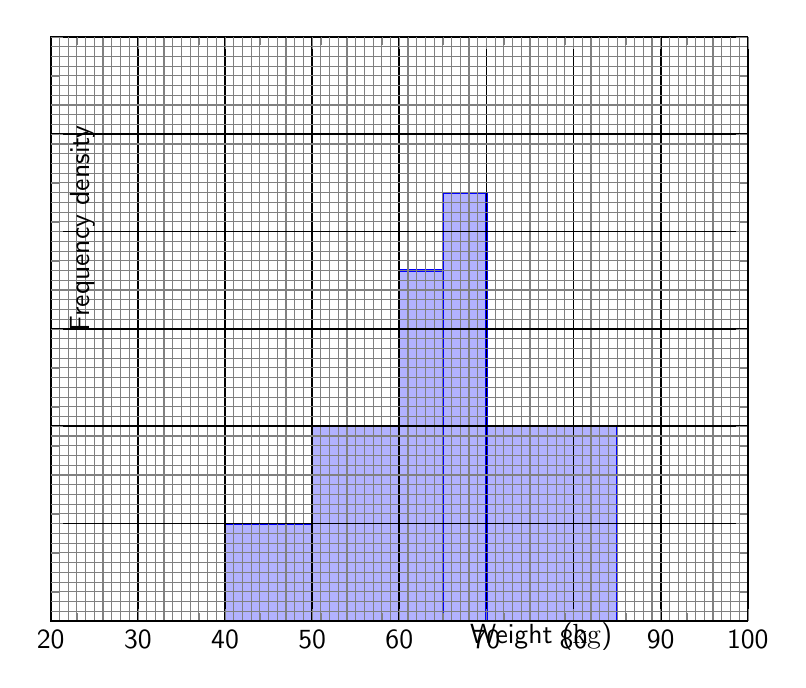
\begin{tikzpicture}
	\centering
	
	\begin{axis}[
	area style,
	height=9cm,
	solid,
	grid = both,
	minor grid style=gray,
	major grid style =black,
	major grid style ={line width =0.6pt},
	xmin = 20, xmax=100,
	ymin=0, ymax= 3,
	minor y tick num=9,
	minor x tick num=9, 
	xtick={20,30,40,50,60,70,80,90,100},
	xticklabels={20,30,40,50,60,70,80,90,100},
	ytick={0,0.5,1,1.5,2,2.5,3},
	yticklabels={\empty,\empty,\empty,\empty,\empty,\empty,\empty}, 	
	x label style={at={(current axis.right of origin)},anchor=north, below=2mm, left =16mm},
	y label style={at={(current axis.above origin)},anchor = west, below =4mm,left = 10mm},
	xlabel={Weight (\si{\kilogram})},
	ylabel={Frequency density}
	]	
	\addplot+[ybar interval,mark=no,thick,solid] plot coordinates { 
		(40,0.5)		
		(50,1)
		(60,1.8)
		(65,2.2)
		(70,1)
		(85,0)		
	};	
	\end{axis}
	\end{tikzpicture}
	
 Compile a grouped frequency table and find an estimate of the mean weight of these students.	

\end{enumerate}


\newpage

%%%%%%%%%%%%%%%%%%%%%%%%%%%%%%%%%%%%%%%%%%%%%
%%%%%%%%%%%%%%%%%%%%%%%%%%%%%%%%%%%%%%%%%%%%%
%%%%%%%%%%%%%%%%%%%%%%%%%%%%%%%%%%%%%%%%%%%%%
%%%%%%%%%%%%%%%%%%%%%%%%%%%%%%%%%%%%%%%%%%%%%
%% 1.5 Variation %%%
%%%%%%%%%%%%%%%%%%%%%%%%%%%%%%%%%%%%%%%%%%%%%
%%%%%%%%%%%%%%%%%%%%%%%%%%%%%%%%%%%%%%%%%%%%%
%%%%%%%%%%%%%%%%%%%%%%%%%%%%%%%%%%%%%%%%%%%%%
%%%%%%%%%%%%%%%%%%%%%%%%%%%%%%%%%%%%%%%%%%%%%
\subsection{Variability of data}


Range:


\vspace{1.5cm}

Variation:

\vspace{1.5cm}

Standard deviation:
\vspace{2cm}

Comparing distributions:  the $\underline{\hspace{3 cm}}$ the standard deviation, the $\underline{\hspace{3 cm}}$ there is and the $\underline{\hspace{3 cm}}$ the data are.
\medskip

'Calculation' version of formula for standard deviation: 

\[
\text{s.d.} = \sqrt{\frac{\sum x^2 }{n}  - \bar{x}^2},\quad \text{where} \quad \bar{x} = \frac{\sum x}{n}.
\] 

Standard deviation of a frequency distribution:

\begin{itemize}
	\item Case $1$
	\item Case $2$
\end{itemize}


\exercise  %%%  Exercise 5

\begin{enumerate}
	\item The mean of the numbers $2,3,5,6,8$ is $4.8$. Calculate the standard deviation.
	
	\item  The distribution shows the number of children in $20$ families. The mean number of children in a family is 2.9. Calculate  the range and the standard deviation.
	
		\medskip
	
	\renewcommand{\arraystretch}{1.2} % default is 1.0
	\begin{tabular}{|c|c|c|c|c|c|}
		\hline
		Number of children, $x$ & $ 1$ & $2$ & $3$ & $4$ & $5$ \\ 
		\hline
		Number of families, $f$ & $3$ & $4$ & $8$ & $2$ & $3$ \\ 
		\hline
	\end{tabular}
	
	\smallskip
	
	
	\item  An online test was taken by 115 students. The time spent on each question was recorded by the computer. The following table shows the time taken, in minutes, on the final question.
		\medskip
	
	\renewcommand{\arraystretch}{1.2} % default is 1.0
	\begin{tabular}{|c|c|c|c|c|}
		\hline
		Time (mins) &  $1\leq x <2$ & $2\leq x <3$ & $3\leq x <5$ & $5\leq x <10$  \\ 
		\hline
		Frequency & $16$ & $32$ & $42$ & $25$  \\ 
		\hline
	\end{tabular}
	
	\smallskip
	
	Calculate estimates of the mean and standard deviation of the time spent on the final question.
	
	\item Becky plays a computer game where she fires at a target. Her score is 1 if she hits the target and 0 if she misses it.
	
	She has 30 attempts and hits the target 18 times.
	
	\begin{enumerate}
		\item Find her mean score for the 30 attempts.
		\item Find the variance of her scores for the 30 attempts.
	\end{enumerate} 
	
	
\end{enumerate}


\newpage



\textbf{Combining sets of data}:
\smallskip

In general, for two sets of data, $x$ and $y$:
\[
\text{mean} = \frac{\sum x + \sum y}{n_1+n_2}, \qquad   \text{stand deviation} = \sqrt{\frac{\sum x^2 + \sum y^2}{n_1+n_2}- (\text{mean})^2}. 
\]


\textbf{Coding data}
\smallskip

In general, if each data value is increased by a constant $a$, 

\begin{itemize}
	\setlength\itemsep{0.8em}
	\item  the mean is  $\underline{\hspace{3cm}}$         .  That is 
	\[
	\bar{x} = \frac{\sum (x-a)}{n} +   a.
	\]
	\item   the standard deviation is $\underline{\hspace{2 cm}}$. That is 
	\[
	\text{s.d. of } x = \sqrt{\frac{\sum (x-a)^2}{n} -  \left(\frac{\sum (x-a)}{n}\right)^2}.  
	\]
\end{itemize}


\exercise   %%%  --- Exercise 6

\begin{enumerate}
	\item The ages, $x$ years, of $18$ people attending an evening class are summarized by the following totals:
	\[
	\sum x = 745,  \qquad \sum x^2 = 33951.
	\]
	\begin{enumerate}
		\item Calculate the mean and the standard deviation of the ages of this group of people.
		\item One person leaves the group and the mean age of the remaining $17$ people is exactly $41$ years. Find the age of the person who left and the standard deviation of the ages of the remaining $17$ people.
	\end{enumerate}
	
	
	\item The following table shows the mean and standard deviation of the heights of $20$ boys and $30$ girls.
	
	\medskip
	\begin{table}[!htpb]
		\centering

\begin{tabular}{|c|c|c|} 
	\cline{2-3}
	\multicolumn{1}{l|}{} & Mean   & Standard deviation  \\ 
	\hline
	Boys                  & $160$ \si{\cm}  & $4$ cm               \\ 
	\hline
	Girls~                & $155$ cm & $3.5$ cm              \\
	\hline
\end{tabular}
	\end{table}
Find the mean and standard deviation of the heights of the $50$ children.


\item  Sweets are packed into bags with a nominal weight of 75 grams. Ten bags are picked at random from the production line and weighted. Their weights, in gram, are 

\vspace{5 pt}

\begin{tabular}{cccccccccc}
	\rule[-1ex]{0pt}{2.5ex}  $76.0$ &$74.2$ & $75.1$ & $73.7$ & $72.0$ & $74.3$ & $75.4$ & $74.0$ & $73.1$ & $72.8$ \\

\end{tabular}

\smallskip

	\begin{enumerate}
		\item Use your calculator to find the mean and the standard deviation .
		\item It is later discovered that the scales were reading 3.2 grams below the correct weight.
		\begin{enumerate}
			\item What was the correct mean weight of the $10$ bags?
			\item What was the correct standard deviation of the $10$ bags?
		\end{enumerate}
	\end{enumerate}


\item The time taken, $x$ minutes, by Katy  to do the Sudoku puzzle in a certain newspaper was observed on $20$ occasions. The results are summarised below.
\[
\sum (x-30) = -50   \qquad \qquad \sum (x-30)^2 =562
\]
Find the mean and standard deviation of the time taken by Katy to solve the Sudoku puzzle.




\item  A summary of $24$ observations of $x$ gave the following informations:
\[
\sum (x-a) = -73.2   \qquad \qquad \sum (x-a)^2 =2115
\]
The mean of these values of $x$ is $8.95$.
\begin{enumerate}
	\item Find the value of the constant $a$.
	\item Find the standard deviation of these value of $x$.
\end{enumerate}



\item  Delip measured the speeds, $x$ \si{\km} per hour, of  $70$ cars on a road where the speed limit is $60$ \si{\km} per hour. His results are summarised by  $\displaystyle \sum (x-60) = 245$.

\begin{enumerate}
	\item Calculate the mean speed of these cars.
\end{enumerate}

His friend Sachim used values of $(x-50)$ to calculate the mean

\begin{enumerate}[resume]
	\item  Find $\displaystyle \sum (x-50)$.
	\item The standard deviation of the speeds is $10.6$ \si{\km} per hour. Calculate  $\displaystyle \sum (x-50)^2$.
\end{enumerate}


\item It is known that, for $100$ observations of $x$, the mean $\bar{x} = 25$.

Find 
\begin{enumerate}
	\item $\displaystyle \sum x$, \,\,\, $\displaystyle \sum (x-20)$,  \,\,\,$\displaystyle \sum (x-27)$.
\end{enumerate} 

Given also that the standard deviation of $x$ is $3$, find 

\begin{enumerate}[resume]
	\item $\displaystyle \sum x^2$,  \,\, \, $\displaystyle \sum (x-20)^2$,  \, \,\,$\displaystyle \sum (x-27)^2$.
\end{enumerate}





\end{enumerate}

\newpage

%%%%%%%%%%%%%%%%%%%%%%%%%%%%%%%%%%%%%%%%%%%%%
%%%%%%%%%%%%%%%%%%%%%%%%%%%%%%%%%%%%%%%%%%%%%
%%%%%%%%%%%%%%%%%%%%%%%%%%%%%%%%%%%%%%%%%%%%%
%%%%%%%%%%%%%%%%%%%%%%%%%%%%%%%%%%%%%%%%%%%%%
%% 1.6 Cumulative frequency graph %%%
%%%%%%%%%%%%%%%%%%%%%%%%%%%%%%%%%%%%%%%%%%%%%
%%%%%%%%%%%%%%%%%%%%%%%%%%%%%%%%%%%%%%%%%%%%%
%%%%%%%%%%%%%%%%%%%%%%%%%%%%%%%%%%%%%%%%%%%%%
%%%%%%%%%%%%%%%%%%%%%%%%%%%%%%%%%%%%%%%%%%%%%
\subsection{Cumulative frequency graph}
\smallskip

When a set of data contains extreme values, known as $\underline{\hspace{2 cm}}$, the median is a more informative average and the interquartile range is more-useful measure of spread. 

\medskip

\textbf{Median}: for a set of $n$ numbers arranged in $\underline{\hspace{4 cm}}$.

\begin{itemize}
		\setlength\itemsep{0.8em}
	\item When $n$ is odd, 
	\item  When $n$ is even,
\end{itemize}


\textbf{Quartiles}:

\begin{itemize}
	\setlength\itemsep{0.8em}
	\item Lower quartile, $Q_1$, 
	\item  Upper quartile, $Q_3$, 
	\item  Interquartile range (IQR), 
\end{itemize}
\bigskip


\textbf{Cumulative frequency}: a total frequency up to a particular item. It is particular useful when finding the median and quartiles. 

\medskip  

\begin{itemize}
	\setlength\itemsep{0.8em}
	\item Ungrouped data
	\item  grouped data,  class boundaries.
 
\end{itemize}
\bigskip

\exercise  %%%  -- Exercise 7

\begin{enumerate}
	\item Find the median 	of each of these sets of numbers:
	\begin{enumerate}
		\item $7,7,2,3,4,2,7,9,31$
		\item  $36,41,27, 32,29, 39, 39, 43$
	\end{enumerate}


    \item  To inverstigate hand-eye coordination in reacting to a stimulus, students took part in an experiment where a ruler was dropped and the distance it travelled before the student caught in was measured. The results of $21$ girls and $27$ boys are shown in the back-to-back stem-and-leaf diagram.
    
 \begin{table}[!htpb]
 	\centering
 	\begin{tabular}{lllllll|c|lllllll}
 		\multicolumn{15}{c}{Distance, in~ cm}                                             \\
 		\multicolumn{7}{c}{Girls}   & \multicolumn{1}{c}{} & \multicolumn{7}{c}{Boys}     \\
 		&   &   &   &   &   &   & 4                    & 8 & 9 &   &   &   &   & (2)  \\
 		&   &   &   &   &   &   & 5                    & 0 & 5 & 9 &   &   &   & (3)  \\
 		(1) &   &   &   &   &   & 8 & 6                    & 2 & 4 &   &   &   &   & (2)  \\
 		(5) &   & 5 & 5 & 3 & 2 & 2 & 7                    & 1 & 4 & 5 &   &   &   & (3)  \\
 		(2) &   &   &   &   & 7 & 6 & 8                    & 0 & 2 & 5 & 7 & 8 & 9 & (6)  \\
 		(6) & 9 & 9 & 8 & 4 & 1 & 1 & 9                    & 3 & 3 & 6 &   &   &   & (3)  \\
 		(3) &   &   &   & 9 & 6 & 3 & 10                   & 0 & 0 & 5 & 7 & 8 &   & (5)  \\
 		(3) &   &   &   & 7 & 5 & 3 & 11                   & 2 & 3 &   &   &   &   & (2)  \\
 		(1) &   &   &   &   &   & 4 & 12                   & 7 &   &   &   &   &   & (1)  \\
 				
	\end{tabular}
 \vspace{4 pt}
 
 \fbox{Key:  $8 |6|2$ represents a distance of 6.8 cm for the girls and 6.2 cm for the boys}
 \end{table}


Find the median and interquartile range for both sets of data. Comment on your answers. 


\item  In a survey on the number of absences in the term of the 32 children in a class, the data were recorded in a cumulative frequency table.

	\medskip

\renewcommand{\arraystretch}{1.2} % default is 1.0
\begin{tabular}{|l|c|c|c|c|c|c|c|c|}
	\hline
	Time absent  & $0$ & $\leqslant 1$ & $\leqslant 2$ & $\leqslant 3$ & $\leqslant 4$ &  $\leqslant 5$ & $\leqslant 6$ & $\leqslant 7$  \\ 
	\hline
	Cumulative frequency & $5$ & $11$ & $20$ & $23$ & $27$ & $28$ & $31$ & $32$ \\ 
	\hline
\end{tabular}

\smallskip

\begin{enumerate}
	\item Find the median number of absence.
	\item Find the interquartile range.
	\item Copy and complete this frequency table.
		\medskip
	
	\renewcommand{\arraystretch}{1.2} % default is 1.0
	\begin{tabular}{|l|c|c|c|c|c|c|c|c|}
		\hline
		Time absent  & $0 \,\,$  & $ 1 \,\, $ & $ 2 \,\,$  & $ 3 \,\,$& $  4 \,\, $ &  $5 \,\,$ & $ 6 \,\,$ & $ 7 \,\,$  \\ 
		\hline
		Frequency & & & &&&&&\\ 
		\hline
	\end{tabular}
	
	\smallskip
	
	\item Calculate the mean number of absences per child.
	\item Calculate the standard deviation.
	
	
\end{enumerate}

\item  The cumulative frequency curve has been drawn from information about the amount of time spent by $50$ people in a supermarket on a particular day.

\medskip


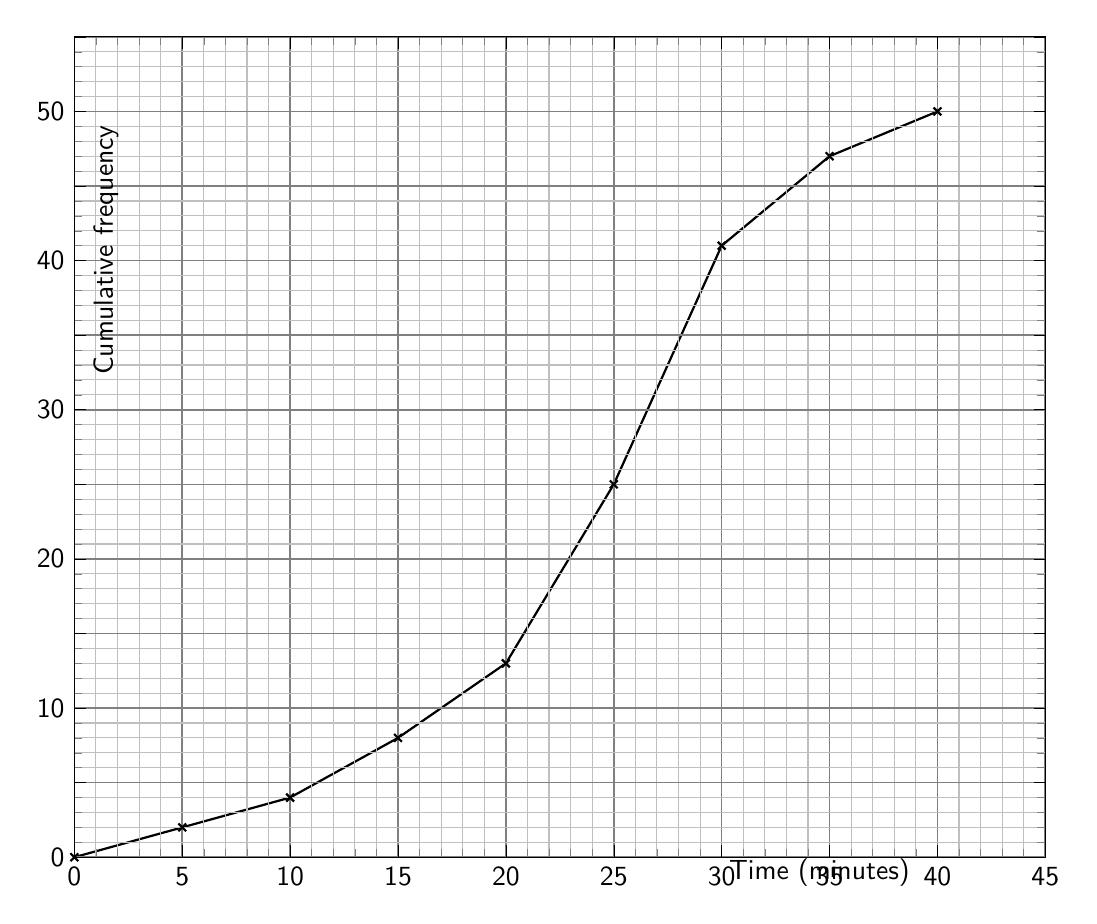
\begin{tikzpicture}
\centering

\begin{axis}[
area style,
height=12cm,
solid,
grid = both,
minor grid style=gray,
major grid style =black,
major grid style ={line width =0.6pt},
%	major grid style =thick,
major tick style=black,	
xmin = 0, xmax=45,
ymin=0, ymax= 55,
grid = both,
minor grid style=lightgray,
major grid style =gray,
major tick style=black,	
minor y tick num=4,
minor x tick num=4, 
xtick={0,5,10,15,20,25,30,35,40,45},
xticklabels={0,5,10,15,20,25,30,35,40,45},
ytick={0,5,10,15,20,25,30,35,40,45,50,55},
yticklabels={0,\empty,10,\empty,20,\empty,30,\empty,40,\empty,50,\empty},
x label style={at={(current axis.right of origin)},anchor=north, below=2mm, left =16mm},
y label style={at={(current axis.above origin)},anchor = west, below =4mm,left = 10mm},
xlabel={Time (minutes)},
ylabel={Cumulative frequency}
]	
\addplot[thick, solid,mark=x] plot coordinates { 
	(0,0)		
	(5,2)
	(10,4)
	(15,8)
	(20,13)
	(25,25)
	(30,41)
	(35,47)
	(40,50)		
};	
\end{axis}
\end{tikzpicture}

\medskip

 Use the graph to estimate
 
 \begin{enumerate}
 	\item how many people spent at least $17$ minutes but less than 27 minutes in the supermarket,
 	\item the value of $t$, where $60\%$ of the people spent less than $t$ minutes in the supermarket,
 	\item the value of $s$, where $60\%$ of the people spent at least $s$ minutes in the supermarket,
 	\item the median time,
 	\item the interquartile range.
 \end{enumerate}


\item  A factory produces certain components. In a quality control test, $500$ components were weighted and their weights recorded to the nearest gram. The table shows the results.

\medskip

\renewcommand{\arraystretch}{1.2} % default is 1.0
\begin{tabular}{|l|c|c|c|c|c|}
	\hline
	Weight (\si{\gram})  & $60-69$ & $70-74$ & $75-79$ & $80-84$ & $85-89$   \\ 
	\hline
	Frequency & $30$ & $90$ & $130$ & $210$ & $40$  \\ 
	\hline
\end{tabular}

\smallskip

\begin{enumerate}
	\item Construct a cumulative frequency table and draw a cumulative frequency graph.
	\item  Components that weight less than $64.5$ grams or more than $87.5$ grams were rejected. Use your graph to estimate the percentage of components that were accepted.
\end{enumerate}



\item  The cumulative frequency table shows the times taken by students to travel to college on a particular day.

\medskip

\renewcommand{\arraystretch}{1.2} % default is 1.0
\begin{tabular}{|l|c|c|c|c|c|}
	\hline
	Time (minutes)  & $ < 10 $ & $ < 15 $ & $ < 20 $ & $ <30 $ & $ <45 $   \\ 
	\hline
	Cumulative frequency & $35$ & $79$ & $157$ & $350$ & $400$  \\ 
	\hline
\end{tabular}

\smallskip

Construct a frequency table and use it to estimate the mean time taken 	to travel to college on that day.


\item The cumulative frequency table gives 	the heights of $400$ children in a certain school.

\medskip

\renewcommand{\arraystretch}{1.2} % default is 1.0
\begin{tabular}{|l|c|c|c|c|c|c|c|c|}
	\hline
	Height, $x$ \si{\cm}  & $ < 100 $ & $ < 110 $ & $ < 120 $ & $ <130 $ & $ <140 $ & $< 150$& $<160$& $<170$   \\ 
	\hline
	Cumulative frequency & $0$ & $27$ & $85$ & $215$ & $320$ & $370$ & $395$ & $400$  \\ 
	\hline
\end{tabular}

\smallskip

\begin{enumerate}
	\item Draw a cumulative frequency curve.
	\item Use the curve to estimate the median height
	\item Determine the interquatile range.
\end{enumerate}

\item The arrival times of $204$ trains were noted and the number of minutes, $t$, that each train was late was recorded.	

\medskip

\renewcommand{\arraystretch}{1.2} % default is 1.0
\begin{tabular}{|l|c|c|c|c|c|}
	\hline
	Number of minutes late ($t$)   & $ -2\leqslant t < 0 $ & $ 0\leqslant t < 2 $ & $ 2\leqslant t < 4 $ & $4\leqslant t < 6 $ & $ 6\leqslant t < 10 $   \\ 
	\hline
	Number of trains & $43$ & $51$ & $69$ & $22$ & $19$  \\ 
	\hline
\end{tabular}

\smallskip

\begin{enumerate}
	\item Explain what $-2\leqslant t <0$ means about the arrival times of the trains.
	\item Draw a cumulative frequency graph, and from it estimate the median and interquartile range of the number of minutes late of these trains.
\end{enumerate}


\item The times, to the nearest minute, taken by $120$ students to write a timed essay were recorded. The results are shown in the table.
 
 \medskip
 
 \renewcommand{\arraystretch}{1.2} % default is 1.0
 \begin{tabular}{|l|c|c|c|c|c|}
 	\hline
 	Time (minutes) ($t$)   & $ 40-44 $ & $ 45-49 $ & $ 50-54 $ & $ 55-59 $ & $ 60-64 $   \\ 
 	\hline
 	Frequency & $8$ & $24$ & $32$ & $30$ & $26$  \\ 
 	\hline
 \end{tabular}
 
 \smallskip
 
 \begin{enumerate}
 	\item Construct the cumulative frequency table and draw a cumulative frequency graph.
 	\item Use your graph to estimate the lower quartile and the median.
 \end{enumerate}

Another group of $40$ students wrote the same essay and all of them took at least 1 hour to complete it.

\begin{enumerate}
	\item Use your graph to estimate the lower quartile of all $160$ students.
	\item Explain why it is not possible to estimate the interquartile range of the times spent by all 160 students.
\end{enumerate}

\end{enumerate}


\newpage

%%%%%%%%%%%%%%%%%%%%%%%%%%%%%%%%%%%%%%%%%%%%%
%%%%%%%%%%%%%%%%%%%%%%%%%%%%%%%%%%%%%%%%%%%%%
%%%%%%%%%%%%%%%%%%%%%%%%%%%%%%%%%%%%%%%%%%%%%
%%%%%%%%%%%%%%%%%%%%%%%%%%%%%%%%%%%%%%%%%%%%%
%% 1.7 Box-and-whisker plot %%%
%%%%%%%%%%%%%%%%%%%%%%%%%%%%%%%%%%%%%%%%%%%%%
%%%%%%%%%%%%%%%%%%%%%%%%%%%%%%%%%%%%%%%%%%%%%
%%%%%%%%%%%%%%%%%%%%%%%%%%%%%%%%%%%%%%%%%%%%%
%%%%%%%%%%%%%%%%%%%%%%%%%%%%%%%%%%%%%%%%%%%%%
\subsection{Box-and-whisker plots}

In a box-and-whisker plot the median and quartiles are shown, as well as the $\underline{\hspace{2 cm}}$ and $\underline{\hspace{2 cm}}$ values of a distribution.

\medskip

For example, 	a survey on the heights of all the girls in a particular year group 	in a school gave the following information.

\begin{tabular}{lc}
	Minimum height  & 144 cm  \\
	Lower quartile~ & 159 cm  \\
	Median~         & 165 cm  \\
	Upper quartile~ & 169 cm  \\
	Maximum height  & 181 cm 
\end{tabular}

A box-and-whisker plot can be drawn as following:

\bigskip
\begin{figure}[!htpb]
\centering
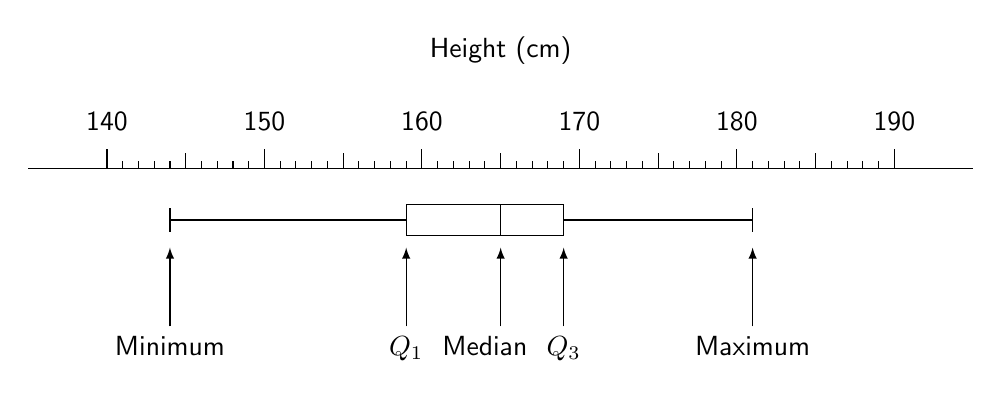
\begin{tikzpicture}

%\def\labelz{{"Judicial Independence","Long Label 2","Label 3","Label 4","180","190"}}
\draw [] (1,0) -- (13,0);
\foreach \x in {1,...,50} {%
	\draw [] (2+0.2*\x,0) -- (2+0.2*\x,0.1);
	
}
\foreach \x in {1,...,10} {%
	\draw [] (2+\x,0) -- (2+\x,0.2);
	
}
\foreach \x in {1,...,6} {%
	\draw [] (2*\x,0) -- (2*\x,0.25);
	\node at (2*\x,0.6){\pgfmathparse{int(130+10*\x)}\pgfmathresult};
}


\draw  (2.8,-0.8) -- (2.8, -0.5);

\draw  (2.8, -0.65) -- (5.8, -0.65);

\draw (5.8,-0.85) rectangle (7.8,-0.45);

\draw (7.8,-0.65) -- (10.2,-0.65);

\draw (10.2,-0.8) -- (10.2,-0.5);

\draw (7,-0.45) -- (7,-0.85);



\draw[-latex] (2.8, -2) -- (2.8,-1) node[below,yshift=-1cm]{Minimum}; 
\draw[-latex] (5.8, -2) -- (5.8,-1) node[below,yshift=-1cm]{ $Q_1$}; 
\draw[-latex] (7, -2) -- (7,-1) node[below,yshift=-1cm,xshift=-0.2cm]{Median}; 
\draw[-latex] (7.8, -2) -- (7.8,-1) node[below,yshift=-1cm]{ $Q_3$}; 
\draw[-latex] (10.2, -2) -- (10.2,-1) node[below,yshift=-1cm]{Maximum}; 

\draw (7,1.5) node{Height (cm)};




\end{tikzpicture} 
\caption{Box-and-whisker plot to show heights of $15$-year-old girl  }

\end{figure}

Tips on drawing the box-and-whisker plot:

\begin{itemize}
	\setlength\itemsep{0.8em}
	\item The scale must be $\underline{\hspace{2 cm}}$ and $\underline{\hspace{2 cm}}$.
	\item The whiskers must not be drawn through the box.
	
\end{itemize}

The shape of a distribution:

\medskip
\vspace{3cm}

Positive skew  \hspace{4.2cm} Symmetrical  \hspace{4.2cm} \hfill Negative skew

\exercise  %%% --  Exercise 8 

\begin{enumerate}
	\item Two groups of people played a computer game which tested  how quickly they reacted to a  visual instruction to press a particular key. The computer measured reaction times in seconds, to the nearest tenth of a second. The following summary statistics were displayed for each group.
	
	\begin{table}[!htpb]
		\centering
		\begin{tabular}{|l|c|c|c|c|c|} 
			\cline{2-6}
			\multicolumn{1}{l|}{} & Minimum & Lower quartile, Q1 & Median, Q2 & Upper quartile, Q3 & Maximum  \\ 
			\hline
			Group 1               & 0.6     & 0.8                & 1.0        & 1.5                & 1.9      \\ 
			\hline
			Group 2               & 0.4     & 0.7                & 1.0        & 1.3                & 1.6      \\
			\hline
		\end{tabular}
	\end{table}

Draw two box-and-whisker plots and compare the reaction time of the two groups.


   \item The following back-to-back stem-and-leaf diagram show the cholesterol count for a group of $45$ people who exercise daily and for another group of $63$ who do not exercise. The figures in brackets show the number of people corresponding to each set of leaves.
  \setlength{\tabcolsep}{1mm}  %% set column width of a table
   \begin{table}[!htpb]
   	\centering
   	\begin{tabular}{lllllllllllll|c|lllllllllllllll}
   		\multicolumn{13}{c}{People who exercise}             & \multicolumn{1}{c}{} & \multicolumn{15}{l}{People who do not exercise}               \\
   		(9)  &   &   &   & 9 & 8 & 7 & 6 & 4 & 3 & 2 & 2 & 1 & 3                    & 1 & 5 & 7 & 7 &   &   &   &   &   &   &   &   &   &   & (4)   \\
   		(12) & 9 & 8 & 8 & 8 & 7 & 6 & 6 & 5 & 3 & 3 & 2 & 2 & 4                    & 2 & 3 & 4 & 4 & 5 & 8 &   &   &   &   &   &   &   &   & (6)   \\
   		(9)  &   &   &   & 8 & 7 & 7 & 7 & 6 & 5 & 3 & 3 & 1 & 5                    & 1 & 2 & 2 & 2 & 3 & 4 & 4 & 5 & 6 & 7 & 8 & 8 & 9 &   & (13)  \\
   		(7)  &   &   &   &   &   & 6 & 6 & 6 & 6 & 4 & 3 & 2 & 6                    & 1 & 2 & 3 & 3 & 3 & 4 & 5 & 5 & 5 & 7 & 7 & 8 & 9 & 9 & (14)  \\
   		(3)  &   &   &   &   &   &   &   &   &   & 8 & 4 & 1 & 7                    & 2 & 4 & 5 & 5 & 6 & 6 & 7 & 8 & 8 &   &   &   &   &   & (9)   \\
   		(4)  &   &   &   &   &   &   &   &   & 9 & 5 & 5 & 2 & 8                    & 1 & 3 & 3 & 4 & 6 & 7 & 9 & 9 & 9 &   &   &   &   &   & (9)   \\
   		(1)  &   &   &   &   &   &   &   &   &   &   &   & 4 & 9                    & 1 & 4 & 5 & 5 & 8 &   &   &   &   &   &   &   &   &   & (5)   \\
   		(0)  &   &   &   &   &   &   &   &   &   &   &   &   & 10                   & 3 & 3 & 6 &   &   &   &   &   &   &   &   &   &   &   & (3)  
   	\end{tabular}
   
    \vspace{4 pt}
   
    
    \fbox{\parbox{3.5in}{Key:  $2 |8|1$ represents a cholesterol count  of 8.2  in the group who exercise 
    		and 8.1 in the group who do not exercise}}
    
  
   \end{table}
	
	
	\begin{enumerate}
		\item Give one useful feature of a stem-and-leaf diagram.
		\item Find the median and quartiles of the cholesterol count for the group who do not exercise.
		
		
	\end{enumerate}
	 
	 You are given that the lower quartile, median and upper quartile of the cholesterol  count for the group who exercise are $4.25$, $5.3$ and $6.6$ respectively.
	 \begin{enumerate}[resume ]
	 	\item On a single diagram on graph, draw two box-and-whisker plots to illustrate the data.
	 \end{enumerate}
 
 \item  The cumulative frequency graph below shows the marks of two groups of 120 people in a test.
 
 \medskip
 
 
 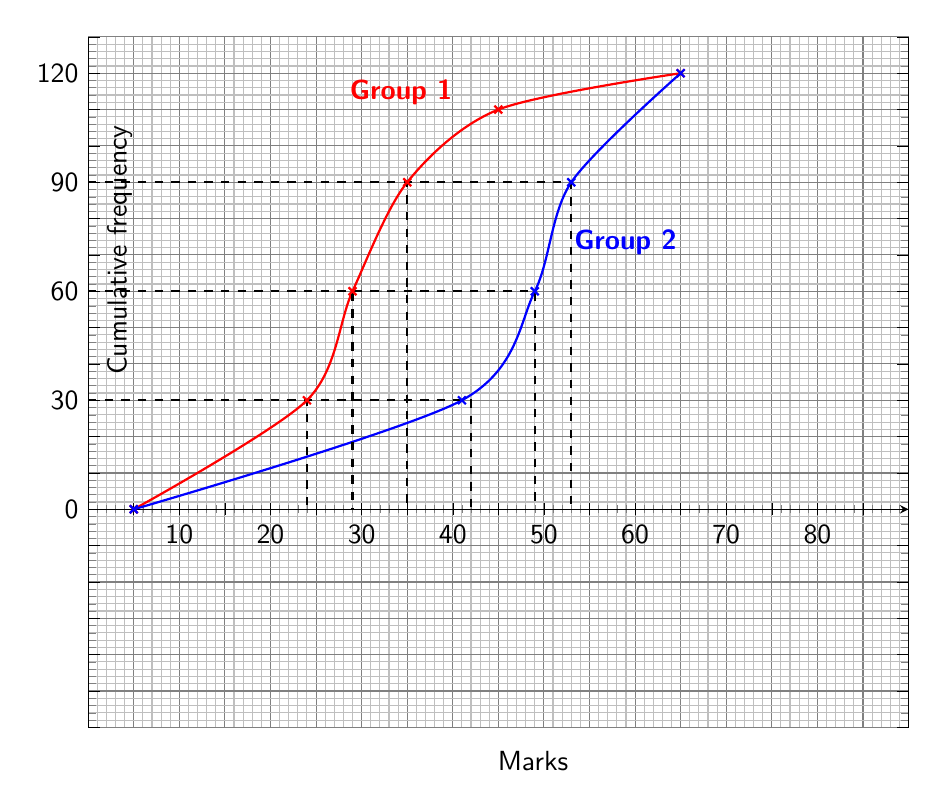
\begin{tikzpicture}
 \centering
 
 \begin{axis}[
 width = 12cm,
 axis x line = middle,
 xmin = 0, xmax=90,
 ymin=-60, ymax= 130,
 grid = both,
 minor grid style=lightgray,
 ytick={-60,-50,-40,-30,-20,-10,0,10,20,30,
 	40,50,60,70,80,90,100,110,120,130},
 yticklabels={\empty,\empty,\empty,\empty,\empty,\empty,0,\empty,\empty,30,
 	          \empty,\empty,60,\empty,\empty,90,\empty,\empty,120,\empty
         },
 xtick={0,5,10,15,20,25,30,35,40,45,50,55,60,65,70,75,80,85,90},
 xticklabels={0,\empty,10,\empty,20,\empty,30,\empty,40,\empty,50,\empty,60,\empty,70,\empty,80,\empty,\empty},
 major grid style =gray,
 major tick style=black,	
 minor x tick num=4,
 minor y tick num=4, 
 %extra x ticks={5,15,25,35,45,},
 %extra x tick labels={5,15,25,35,45},
 %extra y ticks={5,15,25,35,45,55},
 %extra y tick labels={\empty,\empty,\empty,\empty,\empty},
 %extra tick style={
 %	tick style=thick
 %},	
 %yticklabels={\empty,\empty,\empty},
 x label style={at={(current axis.right of origin)},anchor=north, below=3.2cm, left =4.2cm},
 y label style={at={(current axis.above origin)},anchor = west, below =4mm,left = 10mm},
 xlabel={Marks},
 ylabel={Cumulative frequency}
 ]	
 \addplot[thick, mark=x,smooth,red] plot coordinates { 
 	(5,0)		
 	(24,30)
 	(29,60)
 	(35,90)
 	(45,110)
 	(65,120)		
 } node[xshift=-3.55cm,yshift=-0.25cm]{\textbf{Group 1}};	
\addplot[thick, mark=x,smooth,blue] plot coordinates { 
	(5,0)		
	(41,30)
	(49,60)
	(53,90)
	(65,120)		
}node[xshift=-0.7cm,yshift=-2.15cm]{\textbf{Group 2}};	

\addplot[dashed,thick] plot coordinates {
 (0,30)
 (24,30)
 (24,0)
 
};
\addplot[dashed,thick] plot coordinates {
	(0,60)
	(29,60)
	(29,0)
	
};
\addplot[dashed,thick] plot coordinates {
	(0,90)
	(35,90)
	(35,0)
	
};

\addplot[dashed,thick] plot coordinates {
	(0,30)
	(42,30)
	(42,0)
	
};
\addplot[dashed,thick] plot coordinates {
	(0,60)
	(49,60)
	(49,0)
	
};
\addplot[dashed,thick] plot coordinates {
	(0,90)
	(53,90)
	(53,0) 
	
};
 \end{axis}
 \end{tikzpicture}
 
 \medskip
 
 
 Draw two box-and-whisker plots for each group on the same diagram, and compare the two sets of data, state why it is misleading by the cumulative frequency curves.
 
 
	
\end{enumerate}

\newpage 

\subsection{Choosing measures and diagrams}
When representing data  you need to  consider the ways that would be most  appropriate,

\begin{itemize}
\setlength\itemsep{1.8em}
	\item What type of diagram should you draw?
	\item  Which average best represent the data?
	\item Which measure of spread is most informative?
\end{itemize}

\vspace{2cm}
Measure of central tendency:

\begin{table}[!htpb]
	\begin{tabular}{|l|p{6.5cm}|p{6.5cm}|}
		\hline
		& \textbf{Advantages} & \textbf{Disadvantages} \\ \hline
		Mode   &  It is useful when the post popular category is needed.          &  Very small data or more than two modes.
		
			 There may not be a mode.
			 
		 Not representative.
		 
			 The modal class depends on the grouping of data.
	           \\ \hline
		Median &     It is not affected by extreme values.       &   Not use the information of the whole data set            \\ \hline
		Mean   &      Use all the data and so represent every item      &    It is affected by one or two extreme values           \\ \hline
	\end{tabular}
\end{table}

\vspace{2cm}

Measure of spread:

\begin{table}[!htpb]
	\begin{tabular}{|l|p{5.5cm}|p{6cm}|}
		\hline
		& \textbf{Advantages} & \textbf{Disadvantages} \\ \hline
		Range   &  Easy to calculate. 
		
		Represent the complete spread of data.
		         &  It can be affected by extreme values.
		\\ \hline
		Interquartile range &     It is not affected by extreme values.       &   It depends only on particular values when the data was ranked.            \\ \hline
		Standard deviation   &      Use all the data and so represent every item.  
		
		It is useful in comparing two sets of data, to show the consistence.
		    &    It is affected by one or two extreme values.           \\ \hline
	\end{tabular}
\end{table}

\newpage 
Diagrams:

\begin{table}[!htpb]
	\begin{tabular}{|l|p{5cm}|p{5cm}|}
		\hline
		& \textbf{Advantages} & \textbf{Disadvantages} \\ \hline
		
		
		Stem-and-leaf diagram   &  It shows all the original data.
		
		It shows the shape of the distribution.
		
		The mode, median and quartile can be found.
		
		It is useful for comparing two sets of data.
	
		&  It is not suitable for large amount of data.
		\\ \hline
		
		
		Histogram &     It can represent groups of different widths.
		
		It shows whether the distribution is symmetrical or skew
		
		The mean and the standard deviation can be estimated from the histogram.       &   The visual impact can be altered by choosing different groups.
		
		Two distributions cannot be shown on the same diagram.           \\ \hline
		
		
		Cumulative frequency graph   &      The median and quartiles can be estimated the graph.  
		
		Sets of data can be compared by drawing graphs on the same diagram
		&    The visual impact can be altered by using different scales.           \\ \hline
		
		Box-and-whisker plot   &      It is easy to see whether the distribution is symmetrical or whether  there is a tail to the left or right.
		
		It can be used to find the extreme values.
		
		It is easy to see the range and interquartile range.
		
		You can compare two or more sets of data by drawing plots on the same diagram.
		&    It does not show frequencies.           \\ \hline
	\end{tabular}
\end{table}


\newpage

%%%%%%%%% 
%%%%%%%%%
%%%   %%%%%
%%%  Miscelaneous 1
%%%%%%%
%%%%%%%%
%%%%%%%%%%
%%%%%%%%%

\mis

\begin{enumerate}
	
	\item  A company manager, faced with the possibility of having to reduce staff during a recsssion, compiles a table of the ages of his employees.
	
	 \medskip
	
	\renewcommand{\arraystretch}{1.2} % default is 1.0
	\begin{tabular}{|l|c|c|c|c|c|c|}
		\hline
		Age, completed years   & $ 20-30 $ & $ 31-35 $ & $ 36-40 $ & $ 41-45 $ & $ 46-50 $  & $51-60$  \\ 
		\hline
		Number in age group & $5$ & $7$ & $18$ & $30$ & $16$ & $9$ \\ 
		\hline
	\end{tabular}

   \medskip
   
   Draw:
   \begin{enumerate}
   	\item a cumulative frequency graph and so find estimates for the three quartiles,
   	\item a histogram,
   	\item a box-and-whisker plot,
   \end{enumerate}
   to illustreate these figures.
	
	



   \item   The monthly salaries, $w$ dollars, of $10$ women are such that $\displaystyle \sum (w-300) = -200$. 

The monthly salaries, $m$ dollars, of $20$ men are such that $\displaystyle \sum (m-4000) =120$.

\begin{enumerate}
	\item Find the difference between the mean monthly salary of the women and the mean monthly salary of the men.
	\item Find the mean monthly salary of all the women and men together.
\end{enumerate}


\item Eighty candidates took an examination in Astronomy, for which no candidate scored more than $80\%$. The examiners suggest that five grades, $A$, $B$, $C$, $D$ and $E$, should be awarded to these candidates, using upper grade boundaries $64$, $50$, $36$ and $26$ for grades $B$, $C$, $D$ and $E$, respectively. In this case, grades $A$, $B$, $C$, $D$ and $E$, will be awarded in the ratio $1:3:5:4:3$.

\begin{enumerate}
	\item Using the examiners' suggestion, represent the scores in a cumulative frequency graph and use it to estimate the median score.
	\item All of the grade boundaries are later reduced by $10\%$. Estimate how many candidates will be awarded a higher grade because of this.
\end{enumerate}

\item A set of $n$ pieces of data has mean $\bar{x}$ and standard deviation $S$. Another set of $2n$ pieces of data has mean $\bar{x}$ and standard deviation $\frac{1}{2}S$. Find the standard deviation of all these pieces of data together in term of $S$.

\item The daily journey times for $80$ bank staff to get to work are given in the following table.

	 \medskip

\renewcommand{\arraystretch}{1.2} % default is 1.0
\begin{tabular}{|l|c|c|c|c|c|c|c|}
	\hline
	Time ($t$ min)  & $ t<10 $ & $ t<15 $ & $ t<20 $ & $ t<25$ & $ t<30 $  & $t<45$ & $t<60$  \\ 
	\hline
	No.staff (cf) & $3$ & $11$ & $24$ & $56$ & $68$ & $76$  &  $80$ \\ 
	\hline
\end{tabular}

\medskip

\begin{enumerate}
	\item How many staff take between $15$  and $45$ minutes to get to work?
	\item Find the exact number of staff who take $\frac{x+y}{2}$ minutes or more to get to work, given that $85\%$ of the staff take less than $x$ minutes and that $70\%$ of the staff take $y$ minutes or more.
\end{enumerate}



\end{enumerate}










\newpage 
\exam

\begin{enumerate}
	%%%%%%%%%%%%%%%%%%%%%%%%%%%%%%%%%%%%%
	%%%%%%%%%%%%%%%%%%%%%%%%%%%%%%%%%%%%%
	%%%%%%%%%%%%%%%%%%%%%%%%%%%%%%%%%%%%%
	%%% Question 1  9709 s16 qp62  Q2 %%%%
	%%%%%%%%%%%%%%%%%%%%%%%%%%%%%%%%%%%%%
	%%%%%%%%%%%%%%%%%%%%%%%%%%%%%%%%%%%%%
	%%%%%%%%%%%%%%%%%%%%%%%%%%%%%%%%%%%%%
	\item Anabel measured the lengths, in centimetres, of $200$ caterpillars. Her results are illustrated in the	cumulative frequency graph below.
	
	 \medskip
	
	
	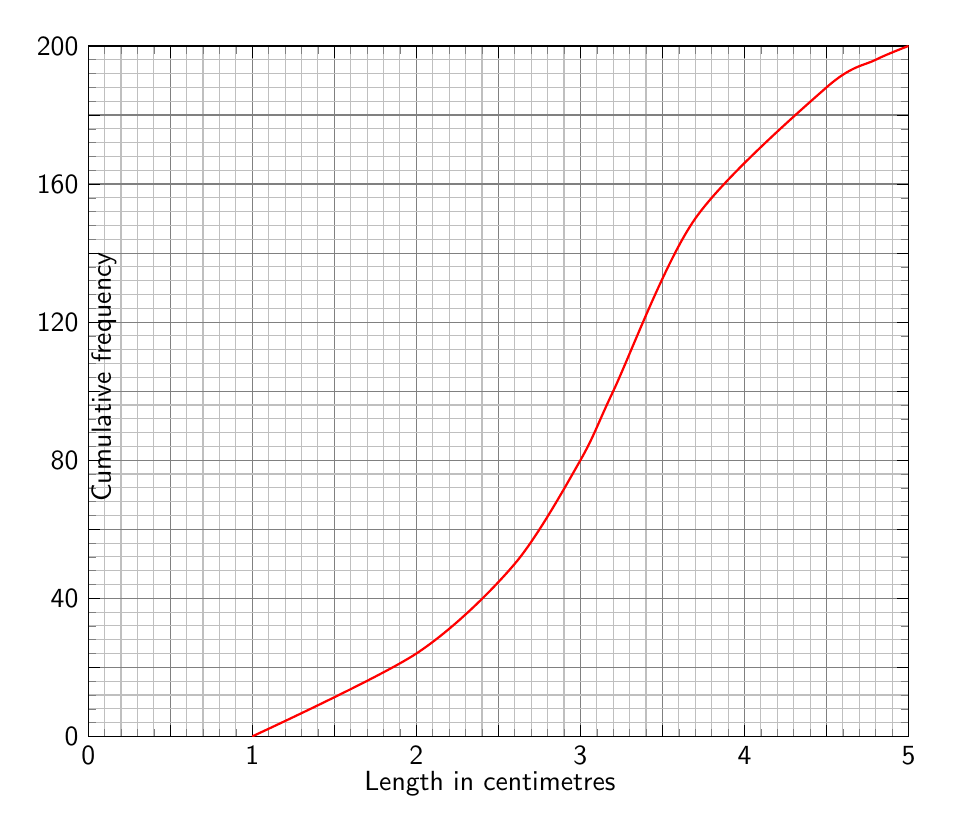
\begin{tikzpicture}
		\centering
		
		\begin{axis}[
			width = 12cm,
			%axis x line = middle,
			xmin = 0, xmax=5,
			ymin=0, ymax= 200,
			grid = both,
			minor grid style=lightgray,
			ytick={0,20,40,60,80,
				100,120,140,160,180,
				200},
			yticklabels={0,\empty,40,\empty,80,
				\empty,120,\empty,160,\empty,
				200
			},
			xtick={0,0.5,1,1.5,2,
				2.5,3,3.5,4,4.5,
				5},
			xticklabels={0,\empty,1,\empty,2,
			\empty,3,\empty,4,\empty,
			5},
			major grid style =gray,
			major tick style=black,	
			minor x tick num=4,
			minor y tick num=4, 
			%extra x ticks={5,15,25,35,45,},
			%extra x tick labels={5,15,25,35,45},
			%extra y ticks={5,15,25,35,45,55},
			%extra y tick labels={\empty,\empty,\empty,\empty,\empty},
			%extra tick style={
			%	tick style=thick
			%},	
			%yticklabels={\empty,\empty,\empty},
			x label style={at={(current axis.right of origin)},anchor=north, below=0.6cm, left =3.6cm},
			y label style={at={(current axis.above origin)},anchor = west, below =2mm,left = 25mm},
			xlabel={Length in centimetres},
			ylabel={Cumulative frequency}
			]	
			\addplot[thick, mark=none,smooth,red] plot coordinates { 
				(1,0)
				(2,24)
				(2.6,50)		
				(3,80)
				(3.2,100)
				(3.7,150)
				(4.5,188)
				(4.8,196)
				(5,200)
						
			} ;	
			
		\end{axis}
	\end{tikzpicture}
	
	\medskip
	
	\begin{enumerate}[label=(\roman*)]
		\item Estimate the median and the interquartile range of the lengths. \hfill [3]
		\item Estimate how many caterpillars had a length of between $2$ and $3.5$ \si{\cm}. \hfill [1]
		\item $6\%$ of caterpillars were of length $l$ centimetres or more. Estimate $l$. \hfill [2]
	\end{enumerate}

%%%%%%%%%%%%%%%%%%%%%%%%%%%%%%%%%%%%%
%%%%%%%%%%%%%%%%%%%%%%%%%%%%%%%%%%%%%
%%%%%%%%%%%%%%%%%%%%%%%%%%%%%%%%%%%%%
%%% Question 2  9709 w18 qp63  Q7 %%%%
%%%%%%%%%%%%%%%%%%%%%%%%%%%%%%%%%%%%%
%%%%%%%%%%%%%%%%%%%%%%%%%%%%%%%%%%%%%
%%%%%%%%%%%%%%%%%%%%%%%%%%%%%%%%%%%%%

\item 



 The heights, in \si{\cm}, of the $11$ members of the Anvils athletics team and the $11$ members of the Brecons swimming team are shown below.
 
 	 \medskip
 
 \renewcommand{\arraystretch}{1.2} % default is 1.0
 \begin{tabular}{|l|c|c|c|c|c|c|c|c|c|c|c|}
 	\hline
 	Anvils  & $ 173 $ & $ 158 $ & $ 180 $ & $ 196$ & $175 $  & $165$ & $170$ & $169$& $181$& $184$ & $172$ \\ 
 	\hline
 	Brecons & $ 166 $ & $ 170 $ & $ 171 $ & $ 172$ & $172 $  & $178$ & $181$ & $182$& $183$& $183$ & $192$ \\ 
 	\hline
 \end{tabular}
 
 \medskip
 
 \begin{enumerate}[label=(\roman*)]
 	\item Draw a back-to-back stem-and-leaf diagram to represent this information, with Anvils on the
 	left-hand side of the diagram and Brecons on the right-hand side. \hfill [4]
 	
 	\item Find the median and the interquartile range for the heights of the Anvils. \hfill [3]
 \end{enumerate}

The heights of the $11$ members of the Anvils are denoted by $x$ \si{\cm}. It is given that $ \sum x =1923$, and  $\sum x^2 =337 221$. Suppose the Anvils are joined by $3$ new members whose heights are $166$ \si{\cm}, $172$ \si{\cm} and $182$ \si{\cm}.

\begin{enumerate}[resume,label=(\roman*)]
	\item Find the standard deviation of the heights of all $14$ members of the Anvils.\hfill  [4]
\end{enumerate}


%%%%%%%%%%%%%%%%%%%%%%%%%%%%%%%%%%%%%
%%%%%%%%%%%%%%%%%%%%%%%%%%%%%%%%%%%%%
%%%%%%%%%%%%%%%%%%%%%%%%%%%%%%%%%%%%%
%%% Question 3  9709 w19 qp62  Q3 %%%%
%%%%%%%%%%%%%%%%%%%%%%%%%%%%%%%%%%%%%
%%%%%%%%%%%%%%%%%%%%%%%%%%%%%%%%%%%%%
%%%%%%%%%%%%%%%%%%%%%%%%%%%%%%%%%%%%%

\item  The speeds, in \si{\km\per\hour}, of $90$ cars as they passed a certain marker on a road were recorded, correct to the nearest \si{\km\per\hour}. The results are summarised in the following table.


\medskip

\renewcommand{\arraystretch}{1.2} % default is 1.0
\begin{tabular}{|l|c|c|c|c|c|}
	\hline
	Speeds (\si{\km\per\hour})  & $ 10-29 $ & $ 30-39 $ & $ 40-49 $ & $ 50-59$ & $60-89$ \\ 
	\hline
	Frequency & $ 10$ & $ 24 $ & $ 30$ & $ 14$ & $12 $ \\ 
	\hline
\end{tabular}

\medskip

\begin{enumerate}[label=(\roman*)]
	\item On the grid, draw a histogram to illustrate the data in the table. \hfill [4]
	\item Calculate an estimate for the mean speed of these $90$ cars as they pass the marker. \hfill [2]
\end{enumerate}


%%%%%%%%%%%%%%%%%%%%%%%%%%%%%%%%%%%%%
%%%%%%%%%%%%%%%%%%%%%%%%%%%%%%%%%%%%%
%%%%%%%%%%%%%%%%%%%%%%%%%%%%%%%%%%%%%
%%% Question 4  9709 s18 qp63  Q4 %%%%
%%%%%%%%%%%%%%%%%%%%%%%%%%%%%%%%%%%%%
%%%%%%%%%%%%%%%%%%%%%%%%%%%%%%%%%%%%%
%%%%%%%%%%%%%%%%%%%%%%%%%%%%%%%%%%%%%

\item  Farfield Travel and Lacket Travel are two travel companies which arrange tours abroad. The numbers
of holidays arranged in a certain week are recorded in the table below, together with the means and
standard deviations of the prices.

\medskip

\begin{table}[!htpb]
	\centering
	\renewcommand{\arraystretch}{1.2} % default is 1.0
	\begin{tabular}{l|c|c|c|}
		\cline{2-4}
		& Number of holidays & Mean price ($\$$) & Standard deviation ($\$$) \\ \hline
		\multicolumn{1}{|l|}{Farfield Travel} & $30$                 & $1500$            & $230 $                    \\ \hline
		\multicolumn{1}{|l|}{Lacket Travel}   & $21$                 & $2400 $           & $160  $                   \\ \hline
	\end{tabular}
\end{table}

\medskip

\begin{enumerate}[label=(\roman*)]
	\item Calculate the mean price of all $51$ holidays. \hfill [2]
	\item The prices of individual holidays with Farfield Travel are denoted by $\$ x_F$	and the prices of
	individual holidays with Lacket Travel are denoted by $\$x_L$. By first finding $\sum x_F^2$ and  $\sum x_L^2$, find the standard deviation of the prices of all $51$ holidays. \hfill[5]
\end{enumerate}


%%%%%%%%%%%%%%%%%%%%%%%%%%%%%%%%%%%%%
%%%%%%%%%%%%%%%%%%%%%%%%%%%%%%%%%%%%%
%%%%%%%%%%%%%%%%%%%%%%%%%%%%%%%%%%%%%
%%% Question 5  9709 s19 qp61  Q4 %%%%
%%%%%%%%%%%%%%%%%%%%%%%%%%%%%%%%%%%%%
%%%%%%%%%%%%%%%%%%%%%%%%%%%%%%%%%%%%%
%%%%%%%%%%%%%%%%%%%%%%%%%%%%%%%%%%%%%

\item The Mathematics and English A-level marks of $1400$ pupils all taking the same examinations are
shown in the cumulative frequency graphs below. Both examinations are marked out of $100$.

\medskip


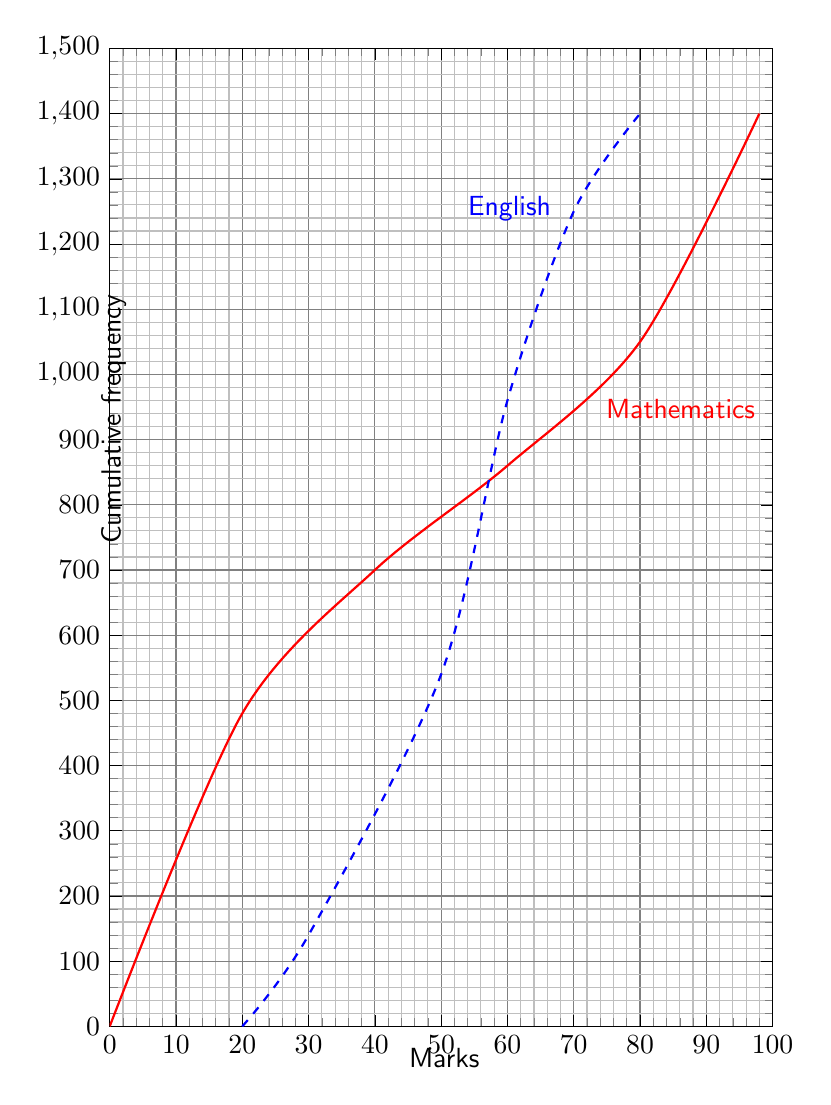
\begin{tikzpicture}
	\centering
	
	\begin{axis}[
		width = 10cm,
		height = 14cm,
		%axis x line = middle,
		xmin = 0, xmax=100,
		ymin=0, ymax= 1500,
		grid = both,
		minor grid style=lightgray,
		ytick={0,100,200,300,400,
			500,600,700,800,900,
			1000,1100,1200,1300,1400,1500},
	%	yticklabels={0,\empty,40,\empty,80,
	%		\empty,120,\empty,160,\empty,
	%		200
	%	},
		xtick={0,10,20,30,40,50,
			60,70,80,90,100},
	%	xticklabels={0,\empty,1,\empty,2,
	%		\empty,3,\empty,4,\empty,
	%		5},
		major grid style =gray,
		major tick style=black,	
		minor x tick num=4,
		minor y tick num=4, 
		%extra x ticks={5,15,25,35,45,},
		%extra x tick labels={5,15,25,35,45},
		%extra y ticks={5,15,25,35,45,55},
		%extra y tick labels={\empty,\empty,\empty,\empty,\empty},
		%extra tick style={
		%	tick style=thick
		%},	
		%yticklabels={\empty,\empty,\empty},
		x label style={at={(current axis.right of origin)},anchor=north, below=0.4cm, left =3.6cm},
		y label style={at={(current axis.above origin)},anchor = west, below =0.5mm,left = 30mm},
		xlabel={Marks},
		ylabel={Cumulative frequency}
		]	
		\addplot[thick, mark=none,smooth,red] plot coordinates { 
			(0,0)
		%	(2,100)
			(20,480)
		%	(30,600)
			(40,700)
			(60,860)
			(80,1050)
			(98,1400)			
		} node[below,yshift=-3.5cm,xshift=-1cm]{Mathematics};	
	\addplot[thick, mark=none,smooth,blue,dashed] plot coordinates { 
		(20,0)
		%	(2,100)
		(30,140)
		%	(30,600)
		(50,540)
		(60,960)
		(70,1250)
		(80,1400)			
	}node[left,xshift=-1.0cm,yshift=-1.2cm]{English} ;	
		
	\end{axis}
\end{tikzpicture}

Use suitable data from these graphs to compare the central tendency and spread of the marks in
Mathematics and English. \hfill [6]


%%%%%%%%%%%%%%%%%%%%%%%%%%%%%%%%%%%%%
%%%%%%%%%%%%%%%%%%%%%%%%%%%%%%%%%%%%%
%%%%%%%%%%%%%%%%%%%%%%%%%%%%%%%%%%%%%
%%% Question 6  9709 w18 qp62  Q2 %%%%
%%%%%%%%%%%%%%%%%%%%%%%%%%%%%%%%%%%%%
%%%%%%%%%%%%%%%%%%%%%%%%%%%%%%%%%%%%%
%%%%%%%%%%%%%%%%%%%%%%%%%%%%%%%%%%%%%

\item The following back-to-back stem-and-leaf diagram shows the reaction times in seconds in an
experiment involving two groups of people, $A$ and $B$.

\begin{table}[!htpb]
	\centering
	 \setlength{\tabcolsep}{2.2mm}  %% set column width of a table
	\begin{tabular}{cllllllll|l|cllllllll}
		\multicolumn{9}{c|}{$A$}              &    & \multicolumn{9}{c}{$B$}               \\ \hline
		(4) &   &   &   &   & 4 & 2 & 0 & 0 & 20 & 5 & 6 & 7 &   &   &   &   &   & (3) \\
		(5) &   &   &   & 9 & 8 & 5 & 0 & 0 & 21 & 1 & 2 & 2 & 3 & 7 & 7 &   &   & (6) \\
		(8) & 9 & 8 & 7 & 5 & 3 & 2 & 2 & 2 & 22 & 1 & 3 & 5 & 6 & 6 & 8 & 9 &   & (7) \\
		(6) &   &   & 8 & 6 & 7 & 5 & 2 & 1 & 23 & 4 & 5 & 7 & 8 & 8 & 9 & 9 & 9 & (8) \\
		(3) &   &   &   &   &   & 8 & 6 & 3 & 24 & 2 & 4 & 5 & 6 & 7 & 8 & 8 &   & (7) \\
		(1) &   &   &   &   &   &   &   & 0 & 25 & 0 & 2 & 7 & 8 &   &   &   &   & (4)
	\end{tabular}

 \vspace{4 pt}


\fbox{\parbox{4.8in}{Key:  $5 |22|6$ means a reaction time of $0.225$ seconds for $A$ and $0.226$ seconds for $B$}}
\end{table}

\begin{enumerate}[label=(\roman*)]
	\item Find the median and the interquartile range for group $A$. \hfill[3]

\end{enumerate}

The median value for group $B$ is $0.235$ seconds, the lower quartile is $0.217$ seconds and the upper
quartile is $0.245$ seconds.

\begin{enumerate}[resume,label=(\roman*)]
	\item Draw box-and-whisker plots for groups $A$ and $B$ on the grid. \hfill [3]
	
	
	\medskip
	\vspace{1cm}
	
	
	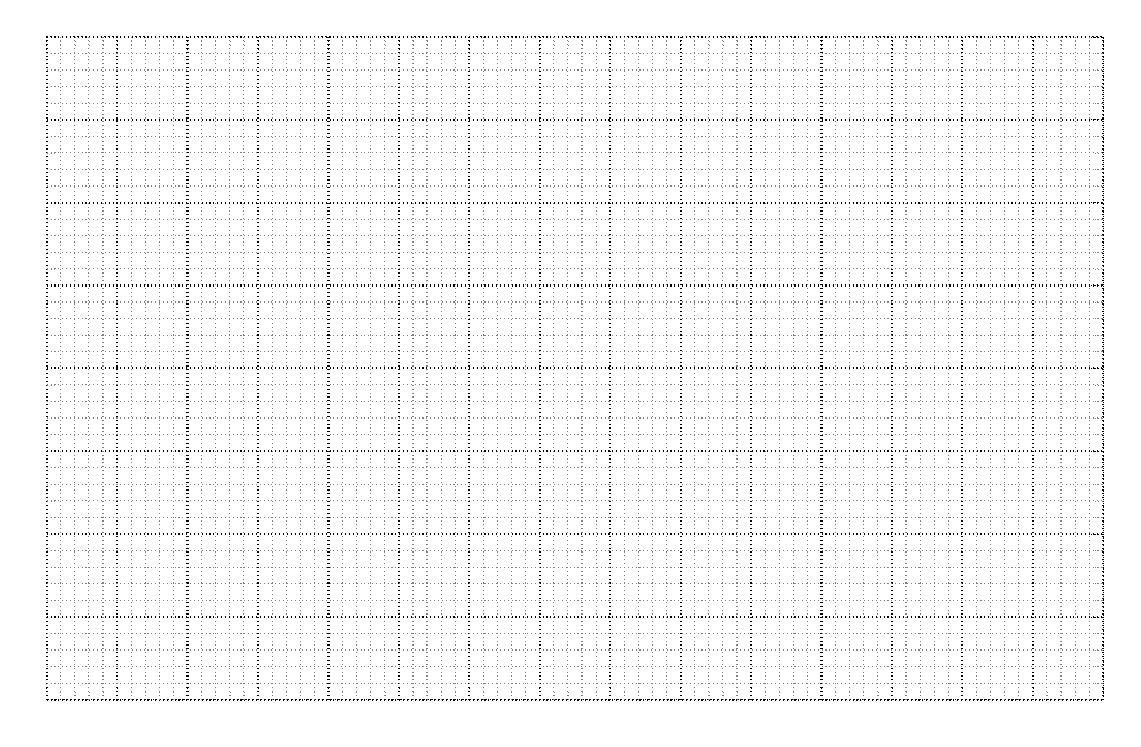
\begin{tikzpicture}
		\centering
		
		\begin{axis}[densely dotted,
			grid = both,
			minor grid style=gray,
			major grid style =black,
			major grid style ={line width =0.8pt},
			%	major grid style =thick,
			major tick style=black,	
			width = 15cm,	
			height = 10cm,		
			%axis x line = middle,
			xmin = 0, xmax=15,
			ymin=0, ymax= 8,			
			ytick={0,1,2,3,4,5,6,7,8},
			yticklabels={\empty,\empty,\empty,\empty,\empty,
				\empty,\empty,\empty,\empty
				},
			xtick={0,1,2,3,4,5,6,7,8,9,10,11,12,13,14,15},
			xticklabels={\empty,\empty,\empty,\empty,
				\empty,\empty,\empty,\empty,
				\empty,\empty,\empty,\empty,
				\empty,\empty,\empty,\empty
			},			
			minor x tick num=4,
			minor y tick num=4, 
			%extra x ticks={5,15,25,35,45,},
			%extra x tick labels={5,15,25,35,45},
			%extra y ticks={5,15,25,35,45,55},
			%extra y tick labels={\empty,\empty,\empty,\empty,\empty},
			%extra tick style={
			%	tick style=thick
			%},	
			%yticklabels={\empty,\empty,\empty},
			x label style={at={(current axis.right of origin)},anchor=north, below=0.4cm, left =3.6cm},
			y label style={at={(current axis.above origin)},anchor = west, below =0.5mm,left = 30mm},
			xlabel={},
			ylabel={}
			]	
		
					\end{axis}
	\end{tikzpicture}
\end{enumerate}







\end{enumerate}

















	\newpage
\section{Permutations and combinations}
%%%%%%%%%%%%%%%%%%%%%%%%%%%%%%%%%%%%%%%%%%%%%
%%%%%%%%%%%%%%%%%%%%%%%%%%%%%%%%%%%%%%%%%%%%%
%%%%%%%%%%%%%%%%%%%%%%%%%%%%%%%%%%%%%%%%%%%%%
%%%%%%%%%%%%%%%%%%%%%%%%%%%%%%%%%%%%%%%%%%%%%
%% 1.1 Arrangements in a line %%%
%%%%%%%%%%%%%%%%%%%%%%%%%%%%%%%%%%%%%%%%%%%%%
%%%%%%%%%%%%%%%%%%%%%%%%%%%%%%%%%%%%%%%%%%%%%
%%%%%%%%%%%%%%%%%%%%%%%%%%%%%%%%%%%%%%%%%%%%%
%%%%%%%%%%%%%%%%%%%%%%%%%%%%%%%%%%%%%%%%%%%%%
\subsection{Arrangements in a line}

\begin{itemize}
	\setlength\itemsep{0.5em}
	\item Arrangements of \textbf{distinct} items	
	
	The number of different arrangements of $n$ distinct items is 
	\[
	n \times (n-1) \times (n-2) \times \ldots \times 3 \times 2 \times 1 = n!	\]
	\item Arrangements when items are \textbf{not} distinct
	
	The number of different arrangements of $n$ items of which $p$ of one type are alike, $q$ of another type are alike, $r$ of another type are alike, and so on, is 
	\[
	\frac{n!}{p!\times q! \times r!\times \ldots}.
	\]
	\item Arrangements when there are restrictions
	\begin{itemize}
			\setlength\itemsep{0.5em}
		\item particular items have to be together, or must be separated.
		\item not all $\&$ all not.
	\end{itemize}
	
	\item Arrangemnets when \textbf{repetitions} are allowed
\end{itemize}

\exercise   %%%%%%%% Exercise 9

\begin{enumerate}
	\item Each of the letters of the word \textbf{CAMBRIDGE} is written on a card and the cards are placed in a line.
	\begin{enumerate}
		\item How many different arrangements are there?
		\item How many arrangements begin with \textbf{CAM}.
	\end{enumerate}

  \item Find the number of different arrangements using all ten letters of the word \textbf{STATISTICS}.
  
  
  \item The word \textbf{ARGENTINA} includes the four consonants \textbf{R}, \textbf{G}, \textbf{N}, \textbf{T} and the three vowels \textbf{A}, \textbf{E},  \textbf{I}.
  \begin{enumerate}
  	\item Find the number of different arrangements using all nine letters.
  	\item How many of these arrangements have a consonant at the beginning, then a vowel, then another consonant, and so on alternately? 
  \end{enumerate}

\item Issam has $11$ different CDs, of which $6$ are pop music, $3$ are jazz and $2$ are classical.
How many different arrangements of all $11$ CDs on a shelf are there if the jazz CDs are all next to each other.

\item The eight sopranos in a choir are asked to stand in a line, but Ruby and Grace refuse to stand next to each other. How many different arrangements can there be?

\item How many $5$-digit \textbf{odd} numbers can be made with the digits $2$, $3$, $6$, $7$, $8$

\begin{enumerate}
	\item if repetitions are not allowed, for example, $63\,287$.
	\item if repetitions are allowed, for example, $88\,663$.
\end{enumerate}


\item  \begin{enumerate}
	\item Safebank requires its customers to use a four-digit PIN to access their account. Customers can choose any set of $4$ digits from $0$, $1$, $2$, $\ldots$, 9 and digits may be repeated. How many possible four-digit PINs are there?
	\item Smartbank requires its customers to use a password consisting of four lower-case letters. Repetitions are allowed. How many  possible passwords are there?
	\item Excelbank requires its customers to use a pass-code consisting of four letters followed by four digits. Repititions are allowed. How many possible pass-codes are there?
\end{enumerate}

\end{enumerate}



\exercise   %%%% -- Exercise 10

\begin{enumerate}
	\item Find the number of ways to arrange the letters of each of the following words:
	\begin{enumerate}
		\item SPIDER
		\item SANDWICH
		\item PENGUIN
		\item BLACKBERRY
		\item MATHEMATICAL
	\end{enumerate}

   \item Find the number of ways in which all eight letters of the word \textbf{ADVANCED} can be arranged if the arrangement must begin and end with an \textbf{A}.
   
   \item Find the number of ways in which all eight letters of the word \textbf{NEEDLESS} can be arranged:
   \begin{enumerate}
   	\item if there are no restrictions,
   	\item if the arrangement must end with \textbf{N},
   	\item if the three letters \textbf{E} must be placed next to each other,
   	\item if the two letters \textbf{S} must  not be placed next to each other,
   	\item if the three letters \textbf{E} must be placed together and the letter \textbf{S} must not be place together.
   \end{enumerate}

\item Five boys and four girls sit on a bench. In how many ways can they be seated if no two boys  sit next to each other?

\item Three identical yellow ballons, two identical red ballons and two identical blue ballons are strung in a row to celebrate Shema's birthday. Calculate the number of arrangements if:

\begin{enumerate}
	\item the ballon at each end is the same colour,
	\item the yellow ballons are next to each other and the blue ballons are not next to each other.
\end{enumerate}

\item Find how many arrangements there are of the nine letters in the word \textbf{GOLD\,MEDAL}

\begin{enumerate}
	\item if there are no restrictions in the order of the letters,
	\item if the two letters \textbf{D} come first and the two letters \textbf{L} come last.
\end{enumerate}


\item Four identical tins of peaches and six identical tins of pears are arranged in a row on a shelf. Calculate the number of different arrangements if the tin at eache end contains the same type of fruit.

\item Three girls and seven boys stand in a line. Calculate the number of different arrangements if:
\begin{enumerate}
	\item the two youngest pupils are separated,
	\item all three girls stand together.
\end{enumerate}

\item There are 10 seats in a row in a theatre. In how many ways can $5$ couples be seated in a row if each couple sits together?

\item Find how many different arrangements there are of eleven letters of the word \textbf{PROBABILITY} if the two letters \textbf{B} are at the beginning and the two letters \textbf{I} are at the end.

\item \boxed{1} \, \boxed{3} \, \boxed{3} \, \boxed{8} \, \boxed{8} \, \boxed{8}

The above cards are placed in a line to form a $6$-digit number. How many numbers can be made:
\begin{enumerate}
	\item if there are no restrictions,
	\item if the number ends in $3$,
	\item if the number is odd?
\end{enumerate}

\end{enumerate}
\newpage
%%%%%%%%%%%%%%%%%%%%%%%%%%%%%%%%%%%%%%%%%%%%%
%%%%%%%%%%%%%%%%%%%%%%%%%%%%%%%%%%%%%%%%%%%%%
%%%%%%%%%%%%%%%%%%%%%%%%%%%%%%%%%%%%%%%%%%%%%
%%%%%%%%%%%%%%%%%%%%%%%%%%%%%%%%%%%%%%%%%%%%%
%% 1.2 Permuations of $r$ items from $n$ items %%%
%%%%%%%%%%%%%%%%%%%%%%%%%%%%%%%%%%%%%%%%%%%%%
%%%%%%%%%%%%%%%%%%%%%%%%%%%%%%%%%%%%%%%%%%%%%
%%%%%%%%%%%%%%%%%%%%%%%%%%%%%%%%%%%%%%%%%%%%%
%%%%%%%%%%%%%%%%%%%%%%%%%%%%%%%%%%%%%%%%%%%%%
\subsection{Permuations of $r$ items from $n$ items}

Suppose $A$, $B$, $C$, $D$, $E$, $F$, $G$ are put into $4$ spaces,
\medskip

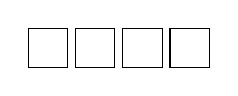
\begin{tikzpicture}
	\draw (-0.25,-0.25) rectangle (0.25,0.25);
	\draw (0.35,-0.25) rectangle (0.85,0.25);
	\draw (0.95,-0.25) rectangle (1.45,0.25);
	\draw (1.55,-0.25) rectangle (2.05,0.25);
\end{tikzpicture}

\medskip

number of ways of arrangements will be $7\times 6 \times 5 \times 4$, which is also denoted by $_{7}\text{P}_4$. Notice that 
\[
7\times 6 \times 5 \times 4=\frac{7\times 6 \times 5 \times 4 \times 3 \times 2 \times 1}{3 \times 2 \times 1} = \frac{7!}{3!} = \frac{7!}{(7-4)!}
\]

In general, the number of permutations, of $r$ items taken from $n$ \textbf{distinct} item is 
\[
_{n}\text{P}_r = \frac{n!}{(n-r)!}.
\]

Special case, $0! =1$.

\medskip

\textbf{Restrictions:}

\begin{itemize}
	\setlength\itemsep{2.5em}
	\item  Not distinct.
	\item  Together.
	\item  others.
	
\end{itemize}

\bigskip

Challenge:  $8$ students sit on $12$ chairs in a row. Among these eight students, $A$ and $B$ must be together. Find the number of different arrangements.

\bigskip

\bigskip

\bigskip

\exercise  %%% Exercise 11
 
\begin{enumerate}
	\item Find how many numbers bigger than $30\,000$ but smaller than $40\,000$ can be formed the digits $2,3,4,5,6,7,8$ if no digit is repeated and the number must be a multiple of $5$. 
	
	\item A security code cosists of $4$ letters chosen from $A$, $B$, $C$, $D$, $E$, $F$, $G$  followed by $3$ digits chosen from $0$, $1$, $2$, $3$, $4$, $5$.
	
	Examples are $BCDG102$ (without repetitions) and $CCDD225$ (with repetitions).
	
	Show that more than five times as many codes can be made when repetitions are allowed than when repetitions are not allowed.
	
	
	\item  Rory is playing a game in which he has to place coloured pegs into holes in a board. He has $6$ identical red pegs and the board has $10$ holes. How many different arrangements are there for placing $6$ pegs and leaving $4$ empty holes?  
	
	\item If repetitions are not allowed, how many numbers can be formed with the digits $3$, $4$, $5$, $6$ $7$ 
	\begin{enumerate}
		\item using three of the digits,
		\item using one or more of the digits? 
	\end{enumerate}


  \item  There are $10$ seats in the front row at a theatre. Six people are shown to this row. In how many different ways can they be seated if 
  \begin{enumerate}
  	\item there are no restrictions,
  	\item two particular people in the group must sit next to each other?
  \end{enumerate}
	
\end{enumerate}


\newpage
%%%%%%%%%%%%%%%%%%%%%%%%%%%%%%%%%%%%%%%%%%%%%
%%%%%%%%%%%%%%%%%%%%%%%%%%%%%%%%%%%%%%%%%%%%%
%%%%%%%%%%%%%%%%%%%%%%%%%%%%%%%%%%%%%%%%%%%%%
%%%%%%%%%%%%%%%%%%%%%%%%%%%%%%%%%%%%%%%%%%%%%
%% 1.2 Combinations of $r$ items from $n$ items %%%
%%%%%%%%%%%%%%%%%%%%%%%%%%%%%%%%%%%%%%%%%%%%%
%%%%%%%%%%%%%%%%%%%%%%%%%%%%%%%%%%%%%%%%%%%%%
%%%%%%%%%%%%%%%%%%%%%%%%%%%%%%%%%%%%%%%%%%%%%
%%%%%%%%%%%%%%%%%%%%%%%%%%%%%%%%%%%%%%%%%%%%%
\subsection{Combinations of $r$ items from $n$ items}

A combination is a selection of some items where the order of the selected item $\underline{\hspace{4cm}}$.

\medskip

In general, the number of combinations of $r$ items from $n$ \textbf{distinct} items is given by

\[
 \binom{n}{r}  =        \, _{n}\text{C}_r       =     \frac{n!}{r!(n-r)!}. 
\]

Notice, "\textbf{distinct}" is a very important conditions for combinations.
\medskip

What happens when the selections are from items that are \textbf{NOT} distinct?

\medskip

For example: Three letters are selected at random from the letters of the word \textbf{BIOLOGY}. Find the total number of selections.

\bigskip

\bigskip

 


\exercise  %%  Exercise 12

\begin{enumerate}
	\item A team of $3$ is to be chosen from $10$ athletes. How many different teams could be chosen?
	
	\item  Without using a calculator, evaluate $\displaystyle \binom{12}{9}$ and $\displaystyle \binom{12}{3}$.
	
	
	\item  Issam has $11$ different CDs of which $6$ are pop music, $3$ are jazz and $2$ are classical. Issam makes a selection of $2$ pop music CDs, $2$ jazz CDs are $1$ classical CD.
	
	
	How many different possible selections can be made?
	
	
	\item A collection of $18$ books contain one Harry Potter book. Linda is going to choose $6$ of these books to take on holiday.
	
	\begin{enumerate}
		\item In how many ways can she choose $6$ books?
		\item How many of these choices will include the Harry Potter book?
	\end{enumerate}


\item  A committee of $5$ people is to be chosen from $6$ men and $4$ women. In how many ways can this be done:

\begin{enumerate}
	\item if there must be $3$ men and $2$  women on the committee,
	\item if there must be more than men than women on the committee,
	\item if there must be $3$ men and $2$ women, and one particular woman refuses to be on the committee with one particular man?
\end{enumerate}


\item In a mixed pack of coloured light bulbs there are three red bulbs, one yellow bulbs, one blue bulbs and one green bulbs. Four bulbs are selected at random from the pack. How many different selections are possible?
	
	
\item  Four letters are to be selected from the letters in the word $RIGIDITY$. How many different combinations are there?	


\item The letters of the word $POSSESSES$ are written on nine cards, one on each card. The cards are shuffled and four of them are selected and arranged in a straight line.
\begin{enumerate}
	\item How many possible selections are there of four letters?
	\item How many arrangments are there of four letters?
\end{enumerate}
\end{enumerate}	
	
\newpage 


	
\mis   %%%%%%%%%  --  miscellaneous 2

%%%%%%%%%%%%%%%%%%%%%%%%
%%%%%%%%%%%%%%%%%%%%%%%%
%%% Q1 m17_qp_62_5 %%%%%
%%%%%%%%%%%%%%%%%%%%%%%%
%%%%%%%%%%%%%%%%%%%%%%%%
%%%%%%%%%%%%%%%%%%%%%%%%
\begin{enumerate}
	\item \begin{enumerate}
		\item A plate of cakes holds $12$ different cakes. Find the number of ways these cakes can be shared between Alex and James if each receives an odd number of cakes. \hfill [3]
		\item Another plate holds $7$ cup cakes, each with a different colour icing, and $4$ brownies, each of a different size. Find the number of different ways these $11$ cakes can be arranged in a row if no	brownie is next to another brownie. \hfill [3]
		\item  A plate of biscuits holds $4$ identical chocolate biscuits, $6$ identical shortbread biscuits and $2$ identical gingerbread biscuits. These biscuits are all placed in a row. Find how many different	arrangements are possible if the chocolate biscuits are all kept together. \hfill [3]
		
			\end{enumerate}
%%%%%%%%%%%%%%%%%%%%%%%%
%%%%%%%%%%%%%%%%%%%%%%%%
%%% Q2 m18_qp_62_2 %%%%%
%%%%%%%%%%%%%%%%%%%%%%%%
%%%%%%%%%%%%%%%%%%%%%%%%
%%%%%%%%%%%%%%%%%%%%%%%%		
		
	\item A selection of $3$ letters from the $8$ letters of the word \textbf{COLLIDER} is made.
	
	\begin{enumerate}
		\item How many different selections of $3$ letters can be made if there is exactly one \textbf{L}? \hfill[1]
		\item How many different selections of $3$ letters can be made if there are no restrictions? \hfill [3]
	\end{enumerate}
		
		
%%%%%%%%%%%%%%%%%%%%%%%%
%%%%%%%%%%%%%%%%%%%%%%%%
%%% Q3 m19_qp_62_7 %%%%%
%%%%%%%%%%%%%%%%%%%%%%%%
%%%%%%%%%%%%%%%%%%%%%%%%
%%%%%%%%%%%%%%%%%%%%%%%%		
		
	\item Find the number of different arrangements that can bemade of all $9$ letters in the word \textbf{CAMERAMAN} in each of the following cases.	
	
  \begin{enumerate}
  	\item There are no restrictions. \hfill[2]
  	\item The \textbf{A}s occupy the $1$st, $5$th and $9$th positions. \hfill[1]
  	\item  There is exactly one letter between the \textbf{M}s. \hfill [4]
  \end{enumerate}
		
		
		
%%%%%%%%%%%%%%%%%%%%%%%%
%%%%%%%%%%%%%%%%%%%%%%%%
%%% Q4 s17_qp_61_7 %%%%%
%%%%%%%%%%%%%%%%%%%%%%%%
%%%%%%%%%%%%%%%%%%%%%%%%
%%%%%%%%%%%%%%%%%%%%%%%%	

\item  \begin{enumerate}
	\item Eight children of different ages stand in a random order in a line. Find the number of different ways this can be done if none of the three youngest children stand next to each other. \hfill[3]
	\item David chooses $5$ chocolates from $6$ different dark chocolates, $4$ different white chocolates and $1$ milk chocolate. He must choose at least one of each type. Find the number of different selections he can make. \hfill[4]
	\item A password for Chelsea’s computer consists of $4$ characters in a particular order. The characters are chosen from the following.
	\begin{itemize}
		\setlength\itemsep{0.5em}
		\item The $26$ capital letters A to Z
		\item The $9$ digits $1$ to $9$
		\item The $5$ symbols $\#$ $\sim$  $*$  $?$  $!$
	\end{itemize} 
	The password must include at least one capital letter, at least one digit and at least one symbol.	No character can be repeated. Find the number of different passwords that Chelsea can make. \hfill 	[4]
\end{enumerate}	
		
%%%%%%%%%%%%%%%%%%%%%%%%
%%%%%%%%%%%%%%%%%%%%%%%%
%%% Q5 s17_qp_62_6 %%%%%
%%%%%%%%%%%%%%%%%%%%%%%%
%%%%%%%%%%%%%%%%%%%%%%%%
%%%%%%%%%%%%%%%%%%%%%%%%	

\item A library contains $4$ identical copies of book A, $2$ identical copies of book B and $5$ identical copies of book C. These $11$ books are arranged on a shelf in the library.

\begin{enumerate}
	\item Calculate the number of different arrangements if the end books are either both book A or both book B. \hfill[4]
	\item Calculate the number of different arrangements if all the books A are next to each other and none of the books B are next to each other. \hfill [5]
\end{enumerate}
	
		
%%%%%%%%%%%%%%%%%%%%%%%%
%%%%%%%%%%%%%%%%%%%%%%%%
%%% Q6 s17_qp_63_6 %%%%%
%%%%%%%%%%%%%%%%%%%%%%%%
%%%%%%%%%%%%%%%%%%%%%%%%
%%%%%%%%%%%%%%%%%%%%%%%%

\item  \begin{enumerate}
	\item Find how many numbers between $3000$ and $5000$ can be formed from the digits $1$, $2$, $3$, $4$ and $5$,
	\begin{enumerate}
		\item if digits are not repeated, \hfill[2] 
		\item if digits can be repeated and the number formed is odd. \hfill[3]
	\end{enumerate}
\item A box of $20$ biscuits contains $4$ different chocolate biscuits, $2$ different oatmeal biscuits and $14$ different ginger biscuits. $6$ biscuits are selected from the box at random.

\begin{enumerate}
	\item Find the number of different selections that include the $2$ oatmeal biscuits. \hfill[2]
	\item Find the probability that fewer than $3$ chocolate biscuits are selected. \hfill[4]
\end{enumerate}

\end{enumerate}		






\end{enumerate}	
	
	
	
	\newpage 
	
	\exam   %%%%  Exam 2
	
	
\begin{enumerate}
	
%%%%%%%%%%%%%%%%%%%%%%%%
%%%%%%%%%%%%%%%%%%%%%%%%
%%% Q1 s18_qp_61_7 %%%%%
%%%%%%%%%%%%%%%%%%%%%%%%
%%%%%%%%%%%%%%%%%%%%%%%%
%%%%%%%%%%%%%%%%%%%%%%%%	
	
	\item Find the number of different ways in which all $9$ letters of the word \textbf{MINCEMEAT} can be arranged in	each of the following cases. 
	\begin{enumerate}[label=(\roman*)]
		\item There are no restrictions.  \hfill[1]
		\item No vowel (\textbf{A}, \textbf{E}, \textbf{I} are vowels) is next to another vowel. \hfill[4]
	\end{enumerate}
    $5$ of the $9$ letters of the word \textbf{MINCEMEAT} are selected.
    \begin{enumerate}[resume,label=(\roman*)]
    	\item Find the number of possible selections which contain exactly $1$ \textbf{M} and exactly $1$ \textbf{E}. \hfill[2]
    	\item  Find the number of possible selections which contain at least $1$ \textbf{M} and at least $1$ \textbf{E}. \hfill[3]
    \end{enumerate}


   
%%%%%%%%%%%%%%%%%%%%%%%%
%%%%%%%%%%%%%%%%%%%%%%%%
%%% Q2 s18_qp_62_6 %%%%%
%%%%%%%%%%%%%%%%%%%%%%%%
%%%%%%%%%%%%%%%%%%%%%%%%
%%%%%%%%%%%%%%%%%%%%%%%%

\item  \begin{enumerate}[label=(\roman*)]
	\item Find the number of ways in which all $9$ letters of the word \textbf{AUSTRALIA} can be arranged in each of the following cases.
	
	\begin{enumerate}[label=(\alph*)]
		\item All the vowels (\textbf{A}, \textbf{I}, \textbf{U} are vowels) are together. \hfill [3]
		\item The letter \textbf{T} is in the central position and each end position is occupied by one of the other consonants (\textbf{R}, \textbf{S}, \textbf{L}). \hfill [3]
	\end{enumerate}
\item Donna has $2$ necklaces, $8$ rings and $4$ bracelets, all different. She chooses $4$ pieces of jewellery.

How many possible selections can she make if she chooses at least $1$ necklace and at least $1$
bracelet?  \hfill [4]
\end{enumerate}


%%%%%%%%%%%%%%%%%%%%%%%%
%%%%%%%%%%%%%%%%%%%%%%%%
%%% Q3 s18_qp_63_7 %%%%%
%%%%%%%%%%%%%%%%%%%%%%%%
%%%%%%%%%%%%%%%%%%%%%%%%
%%%%%%%%%%%%%%%%%%%%%%%%

\item Find the number of ways the $9$ letters of the word \textbf{SEVENTEEN} can be arranged in each of the following cases.

\begin{enumerate}[label=(\roman*)]
	\item One of the letter \textbf{E}s is in the centre with $4$ letters on either side. \hfill[2]
	\item No \textbf{E} is next to another \textbf{E}. \hfill[3]
\end{enumerate}
$5$ letters are chosen from the $9$ letters of the word \textbf{SEVENTEEN}.
\begin{enumerate}[resume,label=(\roman*)]
	\item Find the number of possible selections which contain exactly $2$ \textbf{E}s and exactly 2 \textbf{N}s. \hfill[1]
	\item Find the number of possible selections which contain at least $2$ \textbf{E}s. \hfill[4]
\end{enumerate}

%%%%%%%%%%%%%%%%%%%%%%%%
%%%%%%%%%%%%%%%%%%%%%%%%
%%% Q4 s19_qp_61_7 %%%%%
%%%%%%%%%%%%%%%%%%%%%%%%
%%%%%%%%%%%%%%%%%%%%%%%%
%%%%%%%%%%%%%%%%%%%%%%%%

\item  Freddie has $6$ toy cars and $3$ toy buses, all different. He chooses $4$ toys to take on holiday with him.

\begin{enumerate}[label=(\roman*)]
	\item In how many different ways can Freddie choose $4$ toys? \hfill[1]
	\item How many of these choices will include both his favourite car and his favourite bus? \hfill[2]
\end{enumerate}

Freddie arranges these $9$ toys in a line.

\begin{enumerate}[resume,label=(\roman*)]
	\item Find the number of possible arrangements if the buses are all next to each other. \hfill[3]
	\item  Find the number of possible arrangements if there is a car at each end of the line and no buses are next to each other. \hfill[3]
\end{enumerate}


%%%%%%%%%%%%%%%%%%%%%%%%
%%%%%%%%%%%%%%%%%%%%%%%%
%%% Q5 s19_qp_62_7 %%%%%
%%%%%%%%%%%%%%%%%%%%%%%%
%%%%%%%%%%%%%%%%%%%%%%%%
%%%%%%%%%%%%%%%%%%%%%%%%

\item  \begin{enumerate}[label=(\roman*)]
	\item A group of $6$ teenagers go boating. There are three boats available. One boat has room for $3$ people, one has room for $2$ people and one has room for $1$ person. Find the number of different ways the group of 6 teenagers can be divided between the three boats.\hfill [3]
	\item Find the number of different $7$-digit numbers which can be formed from the seven digits $2$, $2$, $3$, $7$, $7$, $7$, $8$ in each of the following cases.
	\begin{enumerate}[label=(\alph*)]
		\item The odd digits are together and the even digits are together. \hfill [3]
		\item The $2$s are not together. \hfill[4]
	\end{enumerate}
\end{enumerate}


%%%%%%%%%%%%%%%%%%%%%%%%
%%%%%%%%%%%%%%%%%%%%%%%%
%%% Q6 s19_qp_63_7 %%%%%
%%%%%%%%%%%%%%%%%%%%%%%%
%%%%%%%%%%%%%%%%%%%%%%%%
%%%%%%%%%%%%%%%%%%%%%%%%

\item  \begin{enumerate}[label=(\roman*)]
	\item Find the number of ways a committee of $6$ people can be chosen from $8$ men and $4$ women if there must be at least twice as many men as there are women on the committee. \hfill[3]
	\item Find the number of ways a committee of $6$ people can be chosen from $8$ men and $4$ women if $2$ particular men refuse to be on the committee together. \hfill[3]

\end{enumerate}
%%%%%%%%%%%%%%%%%%%%%%%%
%%%%%%%%%%%%%%%%%%%%%%%%
%%% Q7 w17_qp_61_6 %%%%%
%%%%%%%%%%%%%%%%%%%%%%%%
%%%%%%%%%%%%%%%%%%%%%%%%
%%%%%%%%%%%%%%%%%%%%%%%%


\item \begin{enumerate}[label=(\roman*)]
	\item A village hall has seats for $40$ people, consisting of $8$ rows with $5$ seats in each row. Mary,Ahmad, Wayne, Elsie and John are the first to arrive in the village hall and no seats are taken
	before they arrive.
	
	\begin{enumerate}[label=(\alph*)]
		\item How many possible arrangements are there of seatingMary, Ahmad,Wayne, Elsie and John
		assuming there are no restrictions? \hfill[2]
		\item How many possible arrangements are there of seatingMary, Ahmad,Wayne, Elsie and John
		if Mary and Ahmad sit together in the front row and the other three sit together in one of
		the other rows? \hfill[4]
	\end{enumerate}
\item  In how many ways can a team of $4$ people be chosen from 10 people if $2$ of the people, Ross and Lionel, refuse to be in the team together? \hfill [4]
\end{enumerate}



%%%%%%%%%%%%%%%%%%%%%%%%
%%%%%%%%%%%%%%%%%%%%%%%%
%%% Q8 w17_qp_62_6 %%%%%
%%%%%%%%%%%%%%%%%%%%%%%%
%%%%%%%%%%%%%%%%%%%%%%%%
%%%%%%%%%%%%%%%%%%%%%%%%

\item  \begin{enumerate}[label=(\roman*)]
	\item Find the number of different $3$-digit numbers greater than 300 that can be made from the digits $1$, $2$, $3$, $4$, $6$, $8$ if
\begin{enumerate}[label=(\alph*)]
	\item no digit can be repeated, \hfill[3]
	\item a digit can be repeated and the number made is even. \hfill[3]
\end{enumerate}
\item  A team of $5$ is chosen from $6$ boys and $4$ girls. Find the number of ways the team can be chosen if 
\begin{enumerate}[label=(\alph*)]
	\item there are no restrictions, \hfill[1]
	\item the team contains more boys than girls. \hfill[3]
\end{enumerate}
\end{enumerate}



%%%%%%%%%%%%%%%%%%%%%%%%
%%%%%%%%%%%%%%%%%%%%%%%%
%%% Q9 w17_qp_63_6 %%%%%
%%%%%%%%%%%%%%%%%%%%%%%%
%%%%%%%%%%%%%%%%%%%%%%%%
%%%%%%%%%%%%%%%%%%%%%%%%


\item  A car park has spaces for $18$ cars, arranged in a line. On one day there are $5$ cars, of different makes, parked in randomly chosen positions and $13$ empty spaces.

\begin{enumerate}[label=(\roman*)]
	\item Find the number of possible arrangements of the $5$ cars in the car park. \hfill[2]
	\item Find the probability that the $5$ cars are not all next to each other. \hfill[5]
\end{enumerate}
On another day, $12$ cars of different makes are parked in the car park. $5$ of these cars are red, $4$ are white and $3$ are black. Elizabeth selects $3$ of these cars.
\begin{enumerate}[resume,label=(\roman*)]
	\item Find the number of selections Elizabeth can make that include cars of at least $2$ different colours. 
	
	
	\quad \hfill	[5]
\end{enumerate}



%%%%%%%%%%%%%%%%%%%%%%%%
%%%%%%%%%%%%%%%%%%%%%%%%
%%% Q10 w18_qp_61_1 %%%%%
%%%%%%%%%%%%%%%%%%%%%%%%
%%%%%%%%%%%%%%%%%%%%%%%%
%%%%%%%%%%%%%%%%%%%%%%%%

\item  $9$ people are to be divided into a group of $4$, a group of $3$ and a group of $2$. In how many different ways can this be done? \hfill[3]


%%%%%%%%%%%%%%%%%%%%%%%%
%%%%%%%%%%%%%%%%%%%%%%%%
%%% Q11 w18_qp_61_3 %%%%%
%%%%%%%%%%%%%%%%%%%%%%%%
%%%%%%%%%%%%%%%%%%%%%%%%
%%%%%%%%%%%%%%%%%%%%%%%%

\item  In an orchestra, there are $11$ violinists, $5$ cellists and $4$ double bass players. A small group of $6$ musicians is to be selected from these $20$.

\begin{enumerate}[label=(\roman*)]
	\item How many different selections of $6$ musicians can be made if there must be at least $4$ violinists,	at least $1$ cellist and no more than $1$ double bass player? \hfill[4]
\end{enumerate}

The small group that is selected contains $4$ violinists, $1$ cellist and $1$ double bass player. They sit in a line to perform a concert.

\begin{enumerate}[resume,label=(\roman*)]
	\item How many different arrangements are there of these 6musicians if the violinistsmust sit together?
	
	\quad  \hfill	[3]
\end{enumerate}


%%%%%%%%%%%%%%%%%%%%%%%%
%%%%%%%%%%%%%%%%%%%%%%%%
%%% Q12 w18_qp_62_1 %%%%%
%%%%%%%%%%%%%%%%%%%%%%%%
%%%%%%%%%%%%%%%%%%%%%%%%
%%%%%%%%%%%%%%%%%%%%%%%%

\item  \begin{enumerate}[label=(\roman*)]
	\item How many different arrangements are there of the $11$ letters in the word \textbf{MISSISSIPPI}? \hfill[2]
	\item Two letters are chosen at random from the $11$ letters in the word \textbf{MISSISSIPPI}. Find the probability that these two letters are the same. \hfill[3]
\end{enumerate}



%%%%%%%%%%%%%%%%%%%%%%%%
%%%%%%%%%%%%%%%%%%%%%%%%
%%% Q13 w18_qp_62_4 %%%%%
%%%%%%%%%%%%%%%%%%%%%%%%
%%%%%%%%%%%%%%%%%%%%%%%%
%%%%%%%%%%%%%%%%%%%%%%%%

\item  \begin{enumerate}[label=(\roman*)]
	\item  Find the number of different ways that $5$ boys and $6$ girls can stand in a row if all the boys stand together and all the girls stand together. \hfill[3]
	\item Find the number of different ways that $5$ boys and $6$ girls can stand in a row if no boy stands next	to another boy. \hfill[3]
\end{enumerate} 


%%%%%%%%%%%%%%%%%%%%%%%%
%%%%%%%%%%%%%%%%%%%%%%%%
%%% Q14 w18_qp_63_1 %%%%%
%%%%%%%%%%%%%%%%%%%%%%%%
%%%%%%%%%%%%%%%%%%%%%%%%
%%%%%%%%%%%%%%%%%%%%%%%%

\item A group consists of $5$ men and $2$ women. Find the number of different ways that the group can stand in a line if the women are not next to each other. \hfill[3]


%%%%%%%%%%%%%%%%%%%%%%%%
%%%%%%%%%%%%%%%%%%%%%%%%
%%% Q15 w18_qp_63_4 %%%%%
%%%%%%%%%%%%%%%%%%%%%%%%
%%%%%%%%%%%%%%%%%%%%%%%%
%%%%%%%%%%%%%%%%%%%%%%%%
\item  Out of a class of $8$ boys and $4$ girls, a group of $7$ people is chosen at random.

\begin{enumerate}[label=(\roman*)]
	\item Find the probability that the group of $7$ includes one particular boy. \hfill[3]
	\item Find the probability that the group of $7$ includes at least $2$ girls. \hfill [4]
\end{enumerate}




%%%%%%%%%%%%%%%%%%%%%%%%
%%%%%%%%%%%%%%%%%%%%%%%%
%%% Q16 w19_qp_61_6 %%%%%
%%%%%%%%%%%%%%%%%%%%%%%%
%%%%%%%%%%%%%%%%%%%%%%%%
%%%%%%%%%%%%%%%%%%%%%%%%


\item  \begin{enumerate}[label=(\roman*)]
	\item Find the number of different ways in which all $12$ letters of the word \textbf{STEEPLECHASE} can be arranged so that all four \textbf{E}s are together. \hfill[1]
	\item Find the number of different ways in which all $12$ letters of the word \textbf{STEEPLECHASE} can be arranged so that the \textbf{S}s are not next to each other. \hfill [4]
\end{enumerate}
	Four letters are selected from the $12$ letters of the word \textbf{STEEPLECHASE}.
	\begin{enumerate}[resume,label=(\roman*)]
		\item Find the number of different selections if the four letters include exactly one \textbf{S}. \hfill[4]
	\end{enumerate}


%%%%%%%%%%%%%%%%%%%%%%%%
%%%%%%%%%%%%%%%%%%%%%%%%
%%% Q17 w19_qp_62_6 %%%%%
%%%%%%%%%%%%%%%%%%%%%%%%
%%%%%%%%%%%%%%%%%%%%%%%%
%%%%%%%%%%%%%%%%%%%%%%%%

\item  \begin{enumerate}[label=(\roman*)]
	\item Find the number of different ways in which the $9$ letters of the word \textbf{TOADSTOOL} can be	arranged so that all three \textbf{O}s are together and both \textbf{T}s are together. \hfill[1]
	\item Find the number of different ways in which the $9$ letters of the word \textbf{TOADSTOOL} can be arranged so that the \textbf{T}s are not together. \hfill[4]
	\item  Find the probability that a randomly chosen arrangement of the $9$ letters of the word \textbf{TOADSTOOL}	has a \textbf{T} at the beginning and a \textbf{T} at the end. \hfill[2]
	\item Five letters are selected fromthe $9$ letters of the word \textbf{TOADSTOOL}. Find the number of different selections if the five letters include at least $2$ \textbf{O}s and at least $1$ \textbf{T}. \hfill[4]
\end{enumerate}


%%%%%%%%%%%%%%%%%%%%%%%%
%%%%%%%%%%%%%%%%%%%%%%%%
%%% Q18 w19_qp_63_2 %%%%%
%%%%%%%%%%%%%%%%%%%%%%%%
%%%%%%%%%%%%%%%%%%%%%%%%
%%%%%%%%%%%%%%%%%%%%%%%%


\item  \begin{enumerate}[label=(\roman*)]
	\item How many different arrangements are there of the $9$ letters in the word \textbf{CORRIDORS}? \hfill[2]
	\item  How many different arrangements are there of the $9$ letters in the word \textbf{CORRIDORS} in which
	the first letter is \textbf{D} and the last letter is \textbf{R} or \textbf{O}? \hfill [3]
\end{enumerate}


%%%%%%%%%%%%%%%%%%%%%%%%
%%%%%%%%%%%%%%%%%%%%%%%%
%%% Q18 w19_qp_63_3 %%%%%
%%%%%%%%%%%%%%%%%%%%%%%%
%%%%%%%%%%%%%%%%%%%%%%%%
%%%%%%%%%%%%%%%%%%%%%%%%

\item  A sports team of $7$ people is to be chosen from $6$ attackers, $5$ defenders and $4$ midfielders. The team must include at least $3$ attackers, at least $2$ defenders and at least $1$ midfielder.

\begin{enumerate}[label=(\roman*)]
	\item In how many different ways can the team of $7$ people be chosen? \hfill[4]
\end{enumerate}

The team of $7$ that is chosen travels to a match in two cars. A group of $4$ travel in one car and a group of $3$ travel in the other car.

\begin{enumerate}[resume,label=(\roman*)]
	\item In how many different ways can the team of $7$ be divided into a group of $4$ and a group of $3$? \hfill[2]
\end{enumerate}
  













\end{enumerate}	
	
	
	
	
	
	
	
	
	
	
	
	














































	\newpage
\section{Probability}
%%%%%%%%%%%%%%%%%%%%%%%%%%%%%%%%%%%%%%%%%%%%%
%%%%%%%%%%%%%%%%%%%%%%%%%%%%%%%%%%%%%%%%%%%%%
%%%%%%%%%%%%%%%%%%%%%%%%%%%%%%%%%%%%%%%%%%%%%
%%%%%%%%%%%%%%%%%%%%%%%%%%%%%%%%%%%%%%%%%%%%%
%% 3.1 Introduction %%%
%%%%%%%%%%%%%%%%%%%%%%%%%%%%%%%%%%%%%%%%%%%%%
%%%%%%%%%%%%%%%%%%%%%%%%%%%%%%%%%%%%%%%%%%%%%
%%%%%%%%%%%%%%%%%%%%%%%%%%%%%%%%%%%%%%%%%%%%%
%%%%%%%%%%%%%%%%%%%%%%%%%%%%%%%%%%%%%%%%%%%%%
%\setlength\itemsep{0.5em}

\subsection{Introduction}

The probability of an event is  a measure of the likehood that it will happen.

\begin{itemize}
	\setlength\itemsep{0.5em}
	\item A probability of $0$ indicates that the event is $\underline{\hspace{3cm}}$.
	\item A probability of $1$ indicates that the event is $\underline{\hspace{5cm}}$.
	\item All other events have a probability between $\underline{\hspace{1cm}}$ and $\underline{\hspace{1cm}}$.
\end{itemize}

\medskip

\textbf{Notation}

\medskip

The set of all possible outcomes is the \textbf{possibility space}, $S$, and the number of outcomes in the possibility space is written $n(S)$.

\medskip

The event $A$ consists of one or more of the outcomes in $S$. The number of outcomes resulting in event $A$ is written $n(A)$.

\medskip

When outcomes are $\underline{\hspace{4cm}}$, the probability of event $A$ is written $P(A)$ where

\medskip 
\begin{center}
	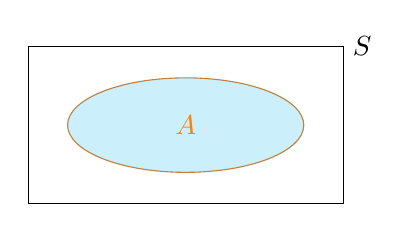
\begin{tikzpicture}
		\draw (0,0) rectangle (4,2) node[right]{$S$};
		\node[ellipse,
		draw = brown,
		text = orange,
		fill = cyan!20,
		minimum width = 3cm, 
		minimum height = 1.2cm] (e) at (2,1) {$A$};
	\end{tikzpicture}
\end{center}


\[
P(A) = \frac{n(A)}{n(S)}.
\]


\exercise  %%%%  --  Exercise 13


\begin{enumerate}
	\item A box contains $20$ counters numbered $1$,$2$,$3$,\ldots, up to $20$. A counter is picked at random from the box. Find the probability that the number on the counter is 
	\begin{enumerate}
		\item  a multiple of $5$,
		\item not a multiple of $5$,
		\item higher than $7$.
	\end{enumerate}



\item   A fair five-sided spinner has sides numbered $1$, $1$, $2$, $3$, $3$. The spinner is spun twice. Find the probability  that the spinner will stop at 1 at  least once.

\medskip

\begin{figure*}[!htpb]
\raggedleft
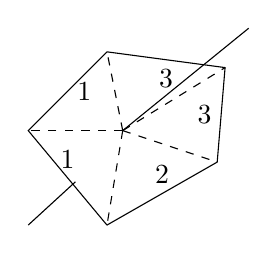
\begin{tikzpicture}	
	\draw (0,0) --node[above]{$2$} (1.4,0.8) -- node[left]{$3$} (1.5,2) -- node[below]{$3$}(0,2.2) -- node[right]{$1$}(-1,1.2) --node[above]{$1$} (0,0);
	
	\draw (0.2,1.2) -- (1.8,2.5);
	\draw (-0.4,0.55) -- (-1,0);
	\draw[dashed] (0.2,1.2) -- (0,0);
	\draw[dashed] (0.2,1.2) -- (1.4,0.8);
	\draw[dashed] (0.2,1.2) -- (1.5,2);
	\draw[dashed] (0.2,1.2) -- (0,2.2);
	\draw[dashed] (0.2,1.2) -- (-1,1.2);
\end{tikzpicture}

\end{figure*}


\item  A card is dealt from a well-shuffled ordinary pack of $52$ playing cards.
\begin{enumerate}
	\item Find the probability that the card is 
	\begin{enumerate}
		\item the $3$ of the spades,
		\item the $3$ of the spades or any diamond.
	\end{enumerate}
\item The first card dealt is placed face-up on the table. It is the $3$ of diamonds. What is the probability that the second card is from a red suit?
\end{enumerate}


\item The table shows the results of all the driving tests taken at a particular test centre during the first week of September. A person is chosen at random from those who took their driving test that week.
\begin{center}

		\begin{tabular}{l|c|c|}
			\cline{2-3}
			& \textbf{Male} & \textbf{Female} \\ \hline
			\multicolumn{1}{|l|}{\textbf{Pass}} & 32            & 43              \\ \hline
			\multicolumn{1}{|l|}{\textbf{Fail}} & 10            & 15              \\ \hline
		\end{tabular}

\end{center}


\begin{enumerate}
	\item Find the probability that the person passed the driving test.
	\item Find the probability that the person is a female who failed the driving test.
	\item A male is chosen. What is the probability that he passed  the driving test.
\end{enumerate}


\item An ordinary tetrahedral die has four faces and they are labelled $1$, $2$, $3$, $4$. When 	the die is thrown, the score is the number on which the die lands. Two fair tetrahedral dice are thrown. By using a possibility space diagram, or otherwise, find the probability that 
\begin{enumerate}
	\item the sum of the scores is divisible by $4$,
	\item the product of the scores is an even number,
	\item the scores differ by at least $2$. 
\end{enumerate} 

\item Two fair coins are tossed together. Find the probability that

\begin{enumerate}
	\item exactly one tail is obtained,
	\item at most one head is obtained.
\end{enumerate}

\item Two ordinary fair cubical dice are thrown. Find the probability that 

\begin{enumerate}
	\item the sum of the numbers on the dice is $3$,
	\item the sum of the numbers on the dice exceeds $9$,
	\item the dice show the same number,
	\item the numbers on the dice differ by more than 2.
\end{enumerate}

\item Two ordinary fair cubical dice are thrown at the same time and the scores are multipled. $\text{P}(N)$ denotes the probability that the number $N$ will be obtained.

\begin{enumerate}
	\item Find 
	\begin{enumerate}
		\item $\text{P}(9)$,
		\item $\text{P}(4)$,
		\item $\text{P}(14)$,
		\item $\text{P}(37)$.
	\end{enumerate}
\item If $\text{P}(N) = \frac{1}{9}$, find the possible values of $N$.
\end{enumerate}

\item Three fair coins are tossed,
\begin{enumerate}
	\item List all possible outcomes,
	\item Find the probability that two heads and one tail are obtained.
\end{enumerate}




\end{enumerate}

\newpage

\subsection{Using permutations and combinations}
%%%%%%%%%%%%%%%%%%%%%%%%%%%%%%%%%%%%%%%%%%%%%
%%%%%%%%%%%%%%%%%%%%%%%%%%%%%%%%%%%%%%%%%%%%%
%%%%%%%%%%%%%%%%%%%%%%%%%%%%%%%%%%%%%%%%%%%%%
%%%%%%%%%%%%%%%%%%%%%%%%%%%%%%%%%%%%%%%%%%%%%
%% 3.2 Using permutations and combinations %%%
%%%%%%%%%%%%%%%%%%%%%%%%%%%%%%%%%%%%%%%%%%%%%
%%%%%%%%%%%%%%%%%%%%%%%%%%%%%%%%%%%%%%%%%%%%%
%%%%%%%%%%%%%%%%%%%%%%%%%%%%%%%%%%%%%%%%%%%%%
%%%%%%%%%%%%%%%%%%%%%%%%%%%%%%%%%%%%%%%%%%%%%
%\setlength\itemsep{0.5em}

In order to find the number of outcomes in a particular event and in the possibility space, you may need to use arrangements permutations and combinations.


\exercise  %%%% --- Exercise 14


\begin{enumerate}
	\item Evan throws three fair dice.
	\begin{enumerate}
		\item List all possible scores on the three dice which give a total of $5$,  and hence show that the probability of Evan obtaining a total score of $5$ is $\frac{1}{36}$.
		\item Find the probability of Evan obtaining a total score of $7$.
	\end{enumerate}

   \item Each of the eleven letters of the word \textbf{MATHEMATICS} is written on a separate card and cards are laid out in a line.
   
   \begin{enumerate}
   	\item Calculate the number of different arrangements of these letters.
   	\item Find the probability that all the vowels are placed together.
   \end{enumerate}


\item Four letters are chosen at random from the letters in the word \textbf{RANDOMLY}. Find the probability that all letters chosen are consonants.

\item A team of $5$ pupils is chosen from a class of $7$ girls and $8$ boys. Find the probability that the team consists of $3$ girls and $2$ boys.

\item  A staff park at a school has $13$ parking spaces in a row.  There are $9$ cars to be parked.
\begin{enumerate}
	\item How many different arrangements are there for parking the $9$ cars and leaving $4$ empty spaces?
	\item How many different arrangements are there if the $4$ empty spaces are next to each other?
	\item If the parking is random, find the probability that there will not be $4$ empty spaces next to each other?
\end{enumerate}


\item  Minerva is given a bag of $20$ sweets of which $6$ are apple flavoured , $6$ are lemon flavoured and $8$ are orange flavoured. Minerva takes out $5$ sweets at random and eats them. Find the probability that she eats:
\begin{enumerate}
	\item $5$ orange flavoured sweets,
	\item $3$ apple flavoured and $2$ lemon flavoured sweets,
	\item exactly $2$ apple flavoured sweets,
	\item no lemon flavoured sweets. 
\end{enumerate}

\item  A plate contains $15$ cakes of which $6$ have yellow icing, $5$ have green icing and $4$ have pink icing.  Three cakes are taken at random from the plate.

Find the probability that:

\begin{enumerate}
	\item exactly two of the cakes have green icing,
	\item one cake has green icing, one has pink icing and one has yellow icing,
	\item none of the cakes has yellow icing.
\end{enumerate}


\item Peter deals a hand of $10$ cards from a well-shuffled pack of ordinary playing cards.	Show the probability that she deals exactly $5$ spades is less than $5\%$.







\end{enumerate}




\newpage

\subsection{Two or more events}
%%%%%%%%%%%%%%%%%%%%%%%%%%%%%%%%%%%%%%%%%%%%%
%%%%%%%%%%%%%%%%%%%%%%%%%%%%%%%%%%%%%%%%%%%%%
%%%%%%%%%%%%%%%%%%%%%%%%%%%%%%%%%%%%%%%%%%%%%
%%%%%%%%%%%%%%%%%%%%%%%%%%%%%%%%%%%%%%%%%%%%%
%%%%%%%% 3.3 Two or more events %%%%%%%%%%%
%%%%%%%%%%%%%%%%%%%%%%%%%%%%%%%%%%%%%%%%%%%%%
%%%%%%%%%%%%%%%%%%%%%%%%%%%%%%%%%%%%%%%%%%%%%
%%%%%%%%%%%%%%%%%%%%%%%%%%%%%%%%%%%%%%%%%%%%%
%%%%%%%%%%%%%%%%%%%%%%%%%%%%%%%%%%%%%%%%%%%%%
%\setlength\itemsep{0.5em}


Now consider two events, $A$ and $B$, in the possibility tree.

\medskip


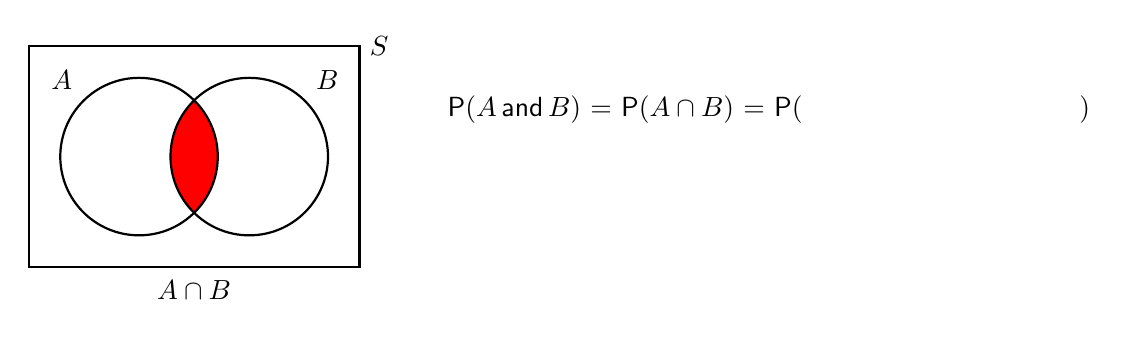
\begin{tikzpicture}[thick,
	set/.style = {circle,
		minimum size = 2cm,
		fill=white}]
	
	% Set A
	\node[set,label={135:$A$}] (A) at (0,0) {};
	
	% Set B
	\node[set,label={45:$B$}] (B) at (1.4,0) {};
	
	% Intersection
	\begin{scope}
		\clip (0,0) circle(1cm);
		\clip (1.4,0) circle(1cm);
		\fill[red](0,0) circle(1cm);
	\end{scope}
	
	% Circles outline
	\draw (0,0) circle(1cm);
	\draw (1.4,0) circle(1cm);
	
	% Set intersection label
	\node at (0.7,-1.7) {$A\cap B$};
	
	\draw (-1.4, -1.4) rectangle (2.8,1.4) node[right]{$S$};
	
	
	\node at (8,0.6) {$\text{P}(A \,\text{and} \, B)$ = $\text{P}(A\cap B)$ = $\text{P}(\qquad \qquad \qquad  \qquad \qquad  )$};
	
\end{tikzpicture}


\medskip

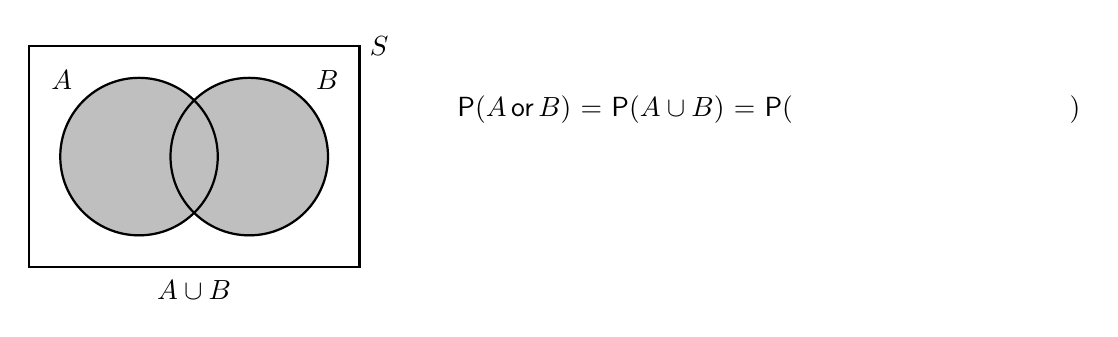
\begin{tikzpicture}[thick,
	set/.style = {circle,
		minimum size = 2cm,
		fill=white}]
	
	% Set A
	\node[set,label={135:$A$}] (A) at (0,0) {};
	
	% Set B
	\node[set,label={45:$B$}] (B) at (1.4,0) {};
	
	% Intersection
%	\begin{scope}
%		\clip (0,0) circle(1cm);
%		\clip (1.4,0) circle(1cm);
%		\fill[red](0,0) circle(1cm);
%	\end{scope}
	
	% Circles outline
	\filldraw[lightgray] (0,0) circle(1cm);
	\filldraw[lightgray] (1.4,0) circle(1cm);
	
		% Circles outline
	\draw (0,0) circle(1cm);
	\draw (1.4,0) circle(1cm);
	
	% Set intersection label
	\node at (0.7,-1.7) {$A\cup B$};
	
	\draw (-1.4, -1.4) rectangle (2.8,1.4) node[right]{$S$};
	
	
	\node at (8,0.6) {$\text{P}(A \,\text{or} \, B)$ = $\text{P}(A\cup B)$ = $\text{P}(\qquad \qquad \qquad  \qquad \qquad  )$};
	
\end{tikzpicture}


\medskip

Addition rule for combined events:

\[
\text{P}(A\, \text{or} \, B) = \text{P}(A) +  \text{P}(B) - \text{P}(A\,\text{and}\, B).
\]

Using set notation:

\[
\text{P}(A\cup  B) = \text{P}(A) +  \text{P}(B) - \text{P}(A \cap B).
\]


\exercise  %%%  -- Exercise 15

\begin{enumerate}
	\item Two events, $X$ and $Y$, are such that $\text{P}( X \, \text{or} \, Y) =0.8$, $\text{P}( X \, \text{and} \, Y) =0.35$ and $\text{P}( X ) =0.6$. Find $\text{P}(Y') $.
	
	\item Events $A$ and $B$ are such that $\text{P}(A \,\text{occurs})=0.6$,  $\text{P}(B \,\text{occurs})=0.7$, $\text{P}(\text{at least one of}\, A \, \text{and}\, B \, \text{occurs})=0.9$.
	
	Find 
	\begin{enumerate}
		\item $\text{P}(\text{both}\, A \, \text{and}\, B \, \text{occur})$.
		\item $\text{P}(\text{neither}\, A \, \text{and}\, B \, \text{occurs})$.
		\item $\text{P}( A \, \text{occurs or}\, B \, \text{occurs but not both} \, A \, \text{and}\, B \, \text{occurs})$
	\end{enumerate}
	
	
	\item   Some pupils did a survey on comics. They asked all $100$ pupils in theri year group whether they read particular comics during the past week. They found that $65$ had read Whizz, $55$ had read Wham, $30$ had read Whizz and Wham and some pupils  in the year group had not read either comic.
	
	A pupil was selected at random from the year group to answer more questions in the survey. Find the probability that the pupil
	
	\begin{enumerate}
		\item had read Whizz or Wham,
		\item had not read either comic.
	\end{enumerate}




\end{enumerate}

\newpage

\textbf{Mutually exclusive events}

\medskip

Events are mutually exclusive $\underline{\text{if they cannot occur at the same time.}}$

\medskip


For example, with one throw of a die, the events 'scoring a $3$' and 'scoring a $5$' are mutually exclusive, since the score cannot be $3$ and $5$ at the same time. 

\medskip 
However, the events 'scoring an even number' and 'scoring a prime number' are not mutually exclusive, since a score of $2$ is both even and prime.


\medskip

\medskip 

Set notation and Venn diagram:

\medskip

When $A$ and $B$ are mutually exclusive there is no overlap between $A$ and $B$.

\begin{figure*}[!htpb]
	\centering
	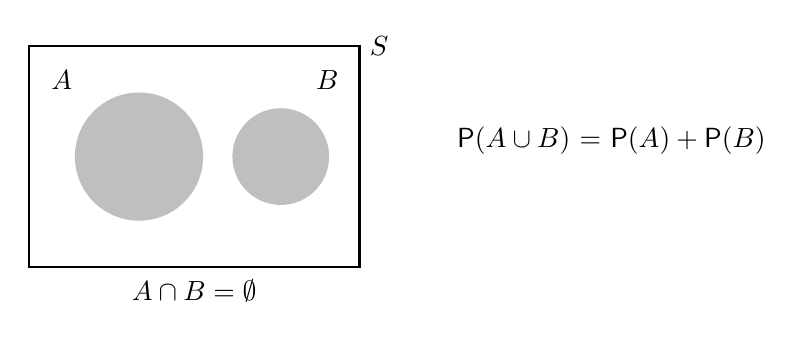
\begin{tikzpicture}[thick,
		set/.style = {circle,
			minimum size = 2cm,
			fill=white}]
		
		% Set A
		\node[set,label={135:$A$}] (A) at (0,0) {};
		
		% Set B
		\node[set,label={45:$B$}] (B) at (1.4,0) {};
		
		% Intersection
		%	\begin{scope}
		%		\clip (0,0) circle(1cm);
		%		\clip (1.4,0) circle(1cm);
		%		\fill[red](0,0) circle(1cm);
		%	\end{scope}
		
		% Circles outline
		\filldraw[lightgray] (0,0) circle(0.8cm);
		\filldraw[lightgray] (1.8,0) circle(0.6cm);
		
		% Circles outline
		%	\draw (0,0) circle(1cm);
		%	\draw (1.4,0) circle(1cm);
		
		% Set intersection label
		\node at (0.7,-1.7) {$A\cap B = \emptyset$};
		
		\draw (-1.4, -1.4) rectangle (2.8,1.4) node[right]{$S$};
		
		
		\node at (6,0.2) {$\text{P}(A\cup B)$ = $\text{P}(A) +  \text{P}(B)$};
		
	\end{tikzpicture}

\end{figure*}

\medskip

Note: if you are asked to show that event $A$ and event $B$ are mutually exclusive, you must give working  to show either the following is satisfied:

\[
\text{P}(A\cup B) = \text{P}(A) +  \text{P}(B) \qquad  \qquad \text{P}(A \cap B) =0.
\]

\exercise  %%%% --------- Exercise 16


\begin{enumerate}
	\item  In a race where there can be only one winner, the probability that John will win is $0.3$,  the probability that Paul will win is $0.2$ and the probability that Mark will win is $0.4$.
	
	Find the probabilibty that 
	
	\begin{enumerate}
		\item John or Mark wins,
		\item John or Paul or Mark wins,
		\item someone else wins.
	\end{enumerate}

\item  A card is dealt from an ordinary pack of $52$ playing cards. Find the probability that the card is 
\begin{enumerate}
	\item a club or a diamond,
	\item a club or a king.
\end{enumerate}

\item Two fair dice are shown.
\begin{enumerate}
	\item Event $A$ is 'the scores differ by $3$ or more'. Find the probability of event $A$.
	\item Event $B$ is 'the product of the scores is greater than $8$'. Find the probability of event $B$.
	\item State with a reason whether events $A$ and $B$ are mutually exclusive.
\end{enumerate}
	
	
	
	
	\item Two fair cubical dice are thrown.
	
	Event $A$ is 'the scores on the dice are the same',
	
	Event $B$ is 'the product of the scores is a multiple of $3$',
	
	Event $C$ is 'the sum of the scores is $7$'.
	
	State with a reason whether $A$ and $B$, $A$ and $C$, $B$ and $C$ are mutually exclusive.
	
	
	
	
\end{enumerate}


\newpage

\subsection{Condtional probability}
%%%%%%%%%%%%%%%%%%%%%%%%%%%%%%%%%%%%%%%%%%%%%
%%%%%%%%%%%%%%%%%%%%%%%%%%%%%%%%%%%%%%%%%%%%%
%%%%%%%%%%%%%%%%%%%%%%%%%%%%%%%%%%%%%%%%%%%%%
%%%%%%%%%%%%%%%%%%%%%%%%%%%%%%%%%%%%%%%%%%%%%
%%%%%%%% 3.4 Conditional probability %%%%%%%%%%%
%%%%%%%%%%%%%%%%%%%%%%%%%%%%%%%%%%%%%%%%%%%%%
%%%%%%%%%%%%%%%%%%%%%%%%%%%%%%%%%%%%%%%%%%%%%
%%%%%%%%%%%%%%%%%%%%%%%%%%%%%%%%%%%%%%%%%%%%%
%%%%%%%%%%%%%%%%%%%%%%%%%%%%%%%%%%%%%%%%%%%%%
%\setlength\itemsep{0.5em}

Condtional probability is used when the probability that an event will occur depends on whether another event has happened.

\medskip

For event $A$ and $B$, the conditional probability that event $B$ occurs, given that $A$ has already occured, i.e.
\[
\text{P}(B \, \text{given}\, A) = \text{P}(B|A)
\]


\medskip
\begin{figure*}[!htpb]
	\centering
	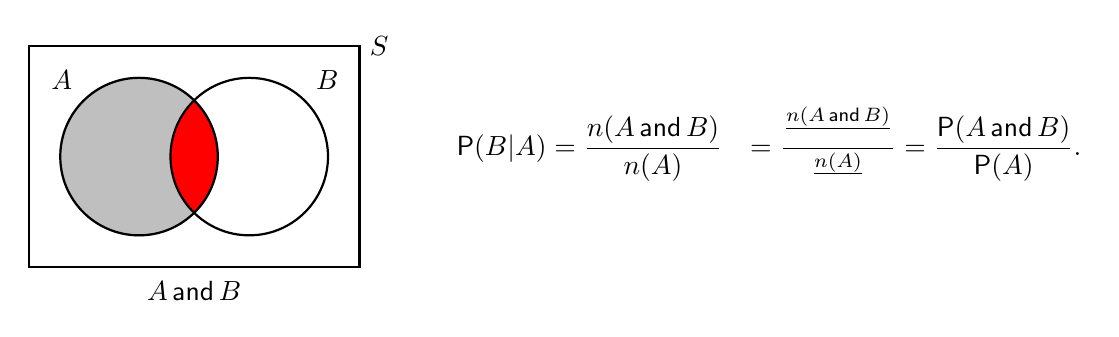
\begin{tikzpicture}[thick,
		set/.style = {circle,
			minimum size = 2cm,
			fill=white}]
		
		% Set A
		\node[set,label={135:$A$}] (A) at (0,0) {};
		
		% Set B
		\node[set,label={45:$B$}] (B) at (1.4,0) {};
		
		
		\filldraw[lightgray] (0,0) circle(1cm);
		% Intersection
		\begin{scope}
			\clip (0,0) circle(1cm);
			\clip (1.4,0) circle(1cm);
			\fill[red](0,0) circle(1cm);
		\end{scope}
		
		% Circles outline
		\draw (0,0) circle(1cm);
		\draw (1.4,0) circle(1cm);
		
		% Set intersection label
		\node at (0.7,-1.7) {$A\, \text{and}\, B$};
		
		\draw (-1.4, -1.4) rectangle (2.8,1.4) node[right]{$S$};
		
		
		\node at (8,0.1) {$\begin{aligned}
				\text{P}(B|A) &= \frac{n(A \, \text{and} \,B )}{n(A)}
				&= \frac{\frac{n(A \, \text{and} \,B )}{\quad}}{\frac{n(A)}{\quad }} 
				& = \frac{\text{P}(A \,\text{and}\, B)}{\text{P}(A)}.\\
			\end{aligned}$};
		
	\end{tikzpicture}
\end{figure*}

This gives the multiplication rule:

\[
\text{P}(A \,\text{and}\, B) =  \text{P}(A) \times  \text{P}(\qquad ).
\]

\exercise  %%   %%%%%%%%%%%% -- Exercise 17

\begin{enumerate}
	\item There are $5$ red counters and $7$ blue counters in a bag. Darian takes  a counter from the bag, puts it on the table and then takes another counter from the bag. Find the probability  that he takes out
	
	\begin{enumerate}
		\item a red counter then a blue counter,
		\item two counters that are the same colour,
		\item at least one red counter.
	\end{enumerate} 


  \item  Two events $X$ and $Y$ are such that $\text{P}(X)=0.2$,  $\text{P}(Y)=0.25$,  $\text{P}(Y|X)=0.4$.
  
  Find 

  \begin{enumerate*}
  	\item $\text{P}(X \,\text{and}\, Y)$,\qquad \,
  	
  	\item $\text{P}(X|Y)$, \qquad \,
  	
  	\item $\text{P}(X \,\text{or}\, Y)$.
  \end{enumerate*}


\item Of the $120$ first year students at a college, $36$ study chemistry, $60$ study biology and $10$ study both chemistry and biology. A first year student is selected at random to represent the college at a conference. Find the probability that the student studies
\begin{enumerate}
	\item chemistry, given that the student studie biology,
	\item biology, given that the student studies  chemistry.
\end{enumerate}

\item Last month a consultant saw $60$ men and $65$ women suspected  of having a particular eye condition. Tests were carried out and the following table shows the results. The totals are shown in bold.

\begin{table}[!htpb]
	\centering
	\begin{tabular}{l|c|c|c}
		\cline{2-3}
		& \textbf{Had eye condition (C)} & \textbf{Did not have eye condition (C')} &                                   \\ \hline
		\multicolumn{1}{|l|}{\textbf{Man (M)}}   & 25                             & 35                                       & \multicolumn{1}{c|}{\textbf{60}}  \\ \hline
		\multicolumn{1}{|l|}{\textbf{Woman (W)}} & 20                             & 45                                       & \multicolumn{1}{c|}{\textbf{65}}  \\ \hline
		& \textbf{45}                    & \textbf{80}                              & \multicolumn{1}{c|}{\textbf{125}} \\ \cline{2-4} 
	\end{tabular}
\end{table}

One of these  patients was selected at random to take part in a survey. Find the probability that the patient selected
\begin{enumerate}
	\item was a women, given that the patient had the eye condition
	\item had the eye condition, given that the patient was a man.
\end{enumerate}




\end{enumerate}

\newpage

\textbf{Independent events}

\medskip

In general, the following rule is correct for any events $A$ and $B$

\[
\text{P}(A \,\text{and}\, B) =  \text{P}(A) \times  \text{P}(B|A).
\]

Now when either of these events can occur without being affected by the outcome of the other,	the events 	are said to be $\underline{\hspace{3cm}}$.

\medskip

So, for \textbf{independent events} $A$ and $B$,

\[
 \text{P}(B|A) = \text{P}(\quad )
\] 
Also

\[
\text{P}(A|B) = \text{P}(\quad )
\]

This gives the multiplication rule for \textbf{independent events}:

\[
\text{P}(A \,\text{and}\, B) =  \text{P}(A) \times  \text{P}(B).
\]

In set notation

\[
\text{P}(\qquad\quad ) =  \text{P}(A) \times  \text{P}(B).
\]

\exercise  %%%%%%%%%%%% --- Exercise 18

\begin{enumerate}
	\item There are $5$ red counters and $7$ blue counters in a bag. Eliza takes a  counter from the bag, notes its colour and then puts it back into the bag. Freddie then takes a counter from the bag. Find the probability that
	\begin{enumerate}
		\item Eliza takes a red counter and Freddie  takes a blue counter,
		\item Freddie's counter is the same colour as Eliza's counter.
	\end{enumerate}


\item Two fair cubical dice are thrown. One is red and the other is blue. Find the probability that 

\begin{enumerate}
	\item the score is $3$ on both dice,
	\item neither die has a score of $3$.
\end{enumerate}


\item The probability that a certain type of machine will break down in the first month of operation is $0.1$. Three machines of this type are installed at the same time. The performances of the three machines are independent. Find the probability that at the end of the first month
\begin{enumerate}
	\item all three machines have broken down,
	\item just one machine has broken down,
	\item at least one machine is working.
\end{enumerate}

\item In a large group of people it is known that $10\%$ have a hot breakfast, $20\%$ have a hot lunch and $25\%$ have a hot breakfast or a hot lunch. Find the probability that a person chosen at random from this group

\begin{enumerate}
	\item has a hot breakfast and a hot lunch.
	\item has a hot lunch, given that the person chosen had a hot breakfast.
\end{enumerate}

\item Two events $A$ and $B$ are such that $\text{P}(A|B) =0.4$, $\text{P}(B|A) =0.25$ and $\text{P}(A \,\text{and} \, B) =0.12$.

\begin{enumerate}
	\item Are $A$ and $B$ independent? Give a reason for your answer.
	\item Find $\text{P}(A \,\text{or} \,B)$.
\end{enumerate}

\newpage 

\item Data about employment for males and females in a small rural area are shown in the table.



\begin{table}[!htpb]
	\centering
	\begin{tabular}{l|c|c|}
		\cline{2-3}
		& \textbf{Unemployed} & \textbf{Employed} \\ \hline
		\multicolumn{1}{|l|}{\textbf{Male}}   & 206                 & 412               \\ \hline
		\multicolumn{1}{|l|}{\textbf{Female}} & 358                 & 305               \\ \hline
	\end{tabular}
\end{table}




A person from this area is chosen at random. Let $M$ be the event that the person is male and let $E$ be the event that the person is employed.

\begin{enumerate}
	\item Find $\text{P}(M)$.
	\item Find $\text{P}(M\,\text{and}\, E)$.
	\item Are $M$ and $E$ independent events? Justify your answer.
	\item 	Given that the person chosen is unemployed, find the probability  that the person is female.
\end{enumerate}






\item Two ordinary fair dice, one red and one blue, are thrown.

Events $A$, $B$ and $C$ are defined as follows:

Event $A$: the number showing on the red die is $5$ or $6$

Event $B$: the total of the numbers showing on the two dice is $7$

Event $C$: the total of the numbers showing on the two dice is $8$

\begin{enumerate}
	\item State, with a reason, which two of the events $A$, $B$ and $C$ are mutually exclusive.
	\item Show that the events $A$ and $B$ are independent.
\end{enumerate}




\item A school has $100$ teachers. In a survey on the use of the school car park, the teachers were asked 	whether they had driven a car to school on a particular day. Of the $70$ full-time teachers, 	$45$ had driven a car to  school and of the $30$ part-time teachers, $12$ had driven a car to school.

\begin{enumerate}
	\item Copy and complete the two-way table, where $C$ denotes the event 'the teacher had driven  a car to school that day'.
	
	\begin{table}[!htpb]
		\centering
		\begin{tabular}{r|c|c|c}
			\cline{2-3}
			& \, \,C \, \, & \, \, C'\,\, & Total                    \\ \hline
			\multicolumn{1}{|r|}{Full-time teacher} &   &    & \multicolumn{1}{c|}{}    \\ \hline
			\multicolumn{1}{|r|}{Part-time teacher} &   &    & \multicolumn{1}{c|}{}    \\ \hline
			Total                                   &   &    & \multicolumn{1}{c|}{100} \\ \cline{2-4} 
		\end{tabular}
	\end{table}
	
	\item Find the probability that a teacher chosen at random
	\begin{enumerate}
		\item is a part-time teacher who had driven a car to school,
		\item is a full-time teacher who had not driven a car to school,
		\item is a full-time teacher or had driven 	a car to school,
		\item is a part-time teacher, given that the teacher had driven a car to school.
	\end{enumerate}

\item Are the events 'the teacher had driven a car to school' and 'the teacher is full-time' independent? Give a reason for your answer.
\item Describe two events that are mutally exclusive.    
	
	
\end{enumerate}
 


\end{enumerate}

\newpage

\subsection{Probability trees}
%%%%%%%%%%%%%%%%%%%%%%%%%%%%%%%%%%%%%%%%%%%%%
%%%%%%%%%%%%%%%%%%%%%%%%%%%%%%%%%%%%%%%%%%%%%
%%%%%%%%%%%%%%%%%%%%%%%%%%%%%%%%%%%%%%%%%%%%%
%%%%%%%%%%%%%%%%%%%%%%%%%%%%%%%%%%%%%%%%%%%%%
%%%%%%%% 3.5 Probability trees %%%%%%%%%%%
%%%%%%%%%%%%%%%%%%%%%%%%%%%%%%%%%%%%%%%%%%%%%
%%%%%%%%%%%%%%%%%%%%%%%%%%%%%%%%%%%%%%%%%%%%%
%%%%%%%%%%%%%%%%%%%%%%%%%%%%%%%%%%%%%%%%%%%%%
%%%%%%%%%%%%%%%%%%%%%%%%%%%%%%%%%%%%%%%%%%%%%
%\setlength\itemsep{0.5em}

A very useful method for tacking many probability problems is to draw a tree diagram. 

\medskip

For example,  a jar contains seven red discs and four white discs. Two disc are selected without replacement.
 
\medskip
A tree diagram can be formed as follows:

\begin{figure*}[!htpb]
	\centering
	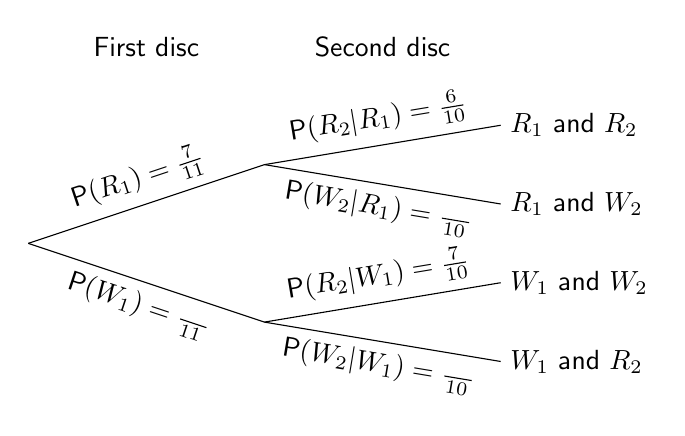
\begin{tikzpicture}
		\draw (0,0) --node[midway,rotate=atan(1/3),above]{$\text{P}(R_1) = \frac{7}{11}$}(3,1) --node[midway,rotate=atan(1/6),above]{$\text{P}(R_2|R_1) = \frac{6}{10}$} (6,1.5) node[right]{$R_1$ and $R_2$};
		\draw         (3,1) --node[midway,rotate=-atan(1/6),below]{$\text{P}(W_2|R_1) = \frac{\quad}{10}$} (6,0.5) node[right]{$R_1$ and $W_2$};
		
		
		
		\draw (0,0) --node[midway,rotate=atan(-1/3),below]{$\text{P}(W_1) = \frac{\quad }{11}$}(3,-1) --node[midway,rotate=-atan(1/6),below]{$\text{P}(W_2|W_1) = \frac{\quad}{10}$} (6,-1.5) node[right]{$W_1$ and $R_2$};
		\draw         (3,-1) -- node[midway,rotate=atan(1/6),above]{$\text{P}(R_2|W_1) = \frac{7}{10}$}(6,-0.5) node[right]{$W_1$ and $W_2$};
		
		\node[] (A) at (1.5,2.5) {First disc};
		
		\node[] (A) at (4.5,2.5) {Second disc};
		
	\end{tikzpicture}
\end{figure*}

then you can find the probability that both of the discs are red by:

\[
\text{P}(R_1\,\text{and}\, R_2) = \text{P}(R_1) \times \text{P}(R_2|R_1) = \qquad  \times \qquad = \qquad .
\]

Meanwhile, the probability of the second discs is red is given by:

\[
\text{P}(R_2) = \text{P}(\qquad \,\text{and}\, R_2) + \text{P}(\qquad \,\text{and}\, R_2) = 
\]


\exercise %%%  -----Exercise 19
 
\begin{enumerate}
	\item In a country $A$ $30\%$ of people who drink tea have sugar in it. In country $B$ $65\%$ of people who drink tea have sugar in it. There are $3$ million in country $A$ who drink tea and $12$ million in country $B$ who drink tea.  A person is chosen at random from these $15$ million people.
	\begin{enumerate}
		\item Find the probability that the person chosen is from country $A$.
		\item Find the probability that the person chosen does not have sugar in their tea.
		\item Given that chosen does not have sugar in their tea, find the probability that the person is from country $B$.
	\end{enumerate}
	
	\item  There are three sets of traffic lights on Karinne's journey to work. The independent probabilities that Karinne has to stop at the first, second and third sets of lights are $0.4$, $0.8$ and $0.3$ respectively.
	\begin{enumerate}
		\item Draw a tree diagram to show this information.
		\item Find the probability that Karinne has to stop at each of the first two sets of lights but does not have to stop at the third set of lights.
		\item Find the probability that Karinne has to stop at exactly two of the three sets of lights.
		\item Find the probability that Karinne has to stop at the first set of lights, given that she has to stop at exactly two sets of lights.
	\end{enumerate}

\item Dan is playing a game in which players pick counters at random, one at a time without replacement, from a bag. At the beginning of the game, the bag contains $6$ red counters and $4$ blue counters. Dan takes two counters from the bag.

\begin{enumerate}
	\item Find the probability that both counters are blue.
	\item Find the probability that the counters are the same color.
	\item Given that the counters are the same color, find the probability that they are both blue.
\end{enumerate} 
	
	
	
	\item When a farmer's dog is let loose, it chases either ducks with probability $\frac{3}{5}$ or geese with probability $\frac{2}{5}$. If the dog chases the ducks, there is a probability of $\frac{1}{10}$ that they will attack the dog. If the dog chases the geese, there is a probability of $\frac{3}{4}$ that they will attack the dog. Given that the dog is not attacked, find the probability that it was chasing the geese. 
	
	
	\item  The probability that Henk goes swimming on any day is $0.2$. On a day that he goes swimming, the probability that Henk has burgers for supper is $0.75$. On a day when he does not go swimming, the probability that he has burgers for his supper is $x$.  The information is shown on the following tree diagram.
	
	\begin{figure*}[!htpb]
		\centering
		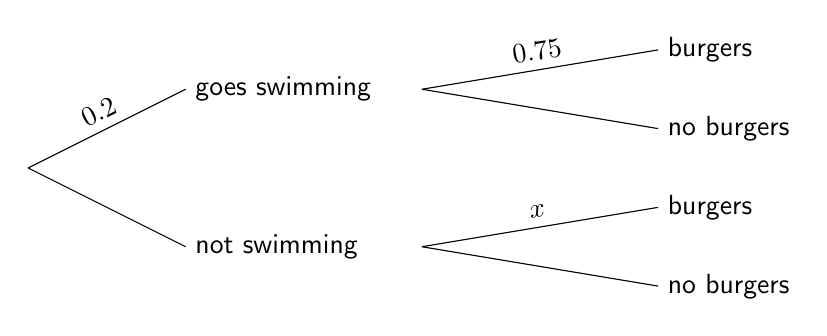
\begin{tikzpicture}
			\draw (0,0) --node[midway,rotate=atan(1/2),above]{$0.2$}(2,1) node[right]{goes swimming};
			
			\draw         (5,1) --node[midway,rotate=atan(1/6),above]{$0.75$} (8,1.5) node[right]{burgers};
			
			\draw         (5,1) -- (8,0.5) node[right]{no burgers};
			
			\draw (0,0) --(2,-1) node[right]{not swimming};
			
			\draw         (5,-1) --node[midway,rotate=atan(1/6),above]{$x$} (8,-0.5) node[right]{burgers};
			
			\draw         (5,-1) -- (8,-1.5) node[right]{no burgers};
	
		\end{tikzpicture}
	\end{figure*}
	
	The probability that Henk has burgers for supper on any day is $0.5$.
	\begin{enumerate}
		\item Find $x$.
		\item Given that Henk has burgers for supper, find the probability that he went swimming that day.
	\end{enumerate}
	
	
	
	\item When Don plays tennis, $65\%$ of his first serves go into the correct are of the court. If the first serve goes into the correct area, his chance of winning the point is $90\%$. If his first serve does not go into the correct area, Don is allowed a second serve and, of these, $80\%$ go into the correct area. If the second serve goes into the correct, his chance of winning the point is $60\%$. If neither serve goes into the correct area, Don loses the point.
	\begin{enumerate}
		\item Draw a tree diagram to represent  this information.
		\item Using the tree diagram, find the probability that Don loses the point.
		\item Find the conditional probability that Don's first serve went into the correct area, given that he loses the point.
	\end{enumerate} 
	
	
	
	\item In an archery competition, Bill is allowed up to three attempts to hit the target. If he succeeds on any attempt, he does not make any more attempts. The probability that he will hit the target on the first attempt is $0.6$. If he misses, the probability that he will hit the target on his second attempt is $0.7$. If he misses on the second attempt, the probability that he will hit the target on his third attempt is $0.8$.
	
	\begin{enumerate}
		\item Draw a fully labelled tree diagram.
		\item Find the probability that Bill will hit the target.
		\item Given that Bill hits the target, find the probability that he made at least two attempts.
	\end{enumerate}


\item Boxes of sweets contain toffees and chocolates. Box $A$ contains $6$ toffees and $4$ chocolates, box $B$ contains $5$ toffees and $3$ chocolates and box $C$ contains $3$ toffees and $7$ chocolates. One of the boxes is chosen at random and two sweets are taken out, one after the other, and eaten.
\begin{enumerate}
	\item Find the probability that they are both toffees.
	\item Given that they are both toffees, find the probability that they both came from box $A$.
\end{enumerate}
	
	
\end{enumerate}	
	
	\newpage
	
	
	
	\mis     %%%%%%%% Miscelaneous 3
	
	\begin{enumerate}
		
		
	%%%%%%%%%%%%%%%%%%%%%%%%%%%%%%%%%%	
	%%%%%%%%%%%%%%%%%%%%%%%%%%%%%%%%%%	
	%%%%%%%%%%%%%%%%%%%%%%%%%%%%%%%%%%	
	%%%%    Q1 m17_qp_62  q2      %%%	
	%%%%%%%%%%%%%%%%%%%%%%%%%%%%%%%%%%	
	%%%%%%%%%%%%%%%%%%%%%%%%%%%%%%%%%%	
	%%%%%%%%%%%%%%%%%%%%%%%%%%%%%%%%%%
		
		\item A bag contains $10$ pink balloons, $9$ yellow balloons, $12$ green balloons and $9$ white balloons. $7$ balloons are selected at random without replacement. Find the probability that exactly $3$ of them are green.  \hfill [3]
		
		
%%%%%%%%%%%%%%%%%%%%%%%%%%%%%%%%%%	
%%%%%%%%%%%%%%%%%%%%%%%%%%%%%%%%%%	
%%%%%%%%%%%%%%%%%%%%%%%%%%%%%%%%%%	
%%%%    Q2 m18_qp_62  q3      %%%	
%%%%%%%%%%%%%%%%%%%%%%%%%%%%%%%%%%	
%%%%%%%%%%%%%%%%%%%%%%%%%%%%%%%%%%	
%%%%%%%%%%%%%%%%%%%%%%%%%%%%%%%%%%		

\item Last Saturday, Sarah recorded the colour and type of $160$ cars in a car park. All the cars that were not red or silver in colour were grouped together as 'other'. Her results are shown in the following table.

	\begin{table}[!htpb]
		\centering
		\begin{tabular}{ll|ccc|}
			\cline{3-5}
			\multicolumn{1}{c}{}                                &        & \multicolumn{3}{c|}{Type of Car}                                      \\ \cline{3-5} 
			\multicolumn{1}{c}{}                                &        & \multicolumn{1}{c|}{Saloon} & \multicolumn{1}{c|}{Hatchback} & Estate \\ \hline
			\multicolumn{1}{|l|}{\multirow{3}{*}{Color of car}} & Red    & \multicolumn{1}{c|}{20}     & \multicolumn{1}{c|}{40}        & 12     \\ \cline{2-5} 
			\multicolumn{1}{|l|}{}                              & Silver & \multicolumn{1}{c|}{14}     & \multicolumn{1}{c|}{26}        & 10     \\ \cline{2-5} 
			\multicolumn{1}{|l|}{}                              & Other  & \multicolumn{1}{c|}{6}      & \multicolumn{1}{c|}{24}        & 8      \\ \hline
		\end{tabular}
	\end{table}

\begin{enumerate}
	\item Find the probability that a randomly chosen car in the car park is a silver estate car. \hfill [1]
	\item Find the probability that a randomly chosen car in the car park is a hatchback car. \hfill[1]
	\item Find the probability that a randomly chosen car in the car park is red, given that it is a hatchback
	car.\hfill [2]
	\item  One of the cars in the car park is chosen at random. Determine whether the events 'the car is a hatchback car' and 'the car is red' are independent, justifying your answer. \hfill [2]
\end{enumerate}
		
		
		
		
%%%%%%%%%%%%%%%%%%%%%%%%%%%%%%%%%%	
%%%%%%%%%%%%%%%%%%%%%%%%%%%%%%%%%%	
%%%%%%%%%%%%%%%%%%%%%%%%%%%%%%%%%%	
%%%%    Q3 s17_qp_61  q2      %%%	
%%%%%%%%%%%%%%%%%%%%%%%%%%%%%%%%%%	
%%%%%%%%%%%%%%%%%%%%%%%%%%%%%%%%%%	
%%%%%%%%%%%%%%%%%%%%%%%%%%%%%%%%%%		

\item	Ashfaq throws two fair dice and notes the numbers obtained. $R$ is the event 'The product of the two numbers is $12$'.  $T$ is the event 'One of the numbers is odd and one of the numbers is even'. By finding appropriate probabilities, determine whether events $R$ and $T$ are independent.	 \hfill  [5]
		
		
		
%%%%%%%%%%%%%%%%%%%%%%%%%%%%%%%%%%	
%%%%%%%%%%%%%%%%%%%%%%%%%%%%%%%%%%	
%%%%%%%%%%%%%%%%%%%%%%%%%%%%%%%%%%	
%%%%    Q4 s17_qp_62  q4      %%%	
%%%%%%%%%%%%%%%%%%%%%%%%%%%%%%%%%%	
%%%%%%%%%%%%%%%%%%%%%%%%%%%%%%%%%%	
%%%%%%%%%%%%%%%%%%%%%%%%%%%%%%%%%%		

\item		Two identical biased triangular spinners with sides marked $1$, $2$ and $3$ are spun. For each spinner, the probabilities of landing on the sides marked $1$, $2$ and $3$ are $p$, $q$ and $r$ respectively. The score is the sum of the numbers on the sides on which the spinners land. You are given that P(score is $6$) = $\frac{1}{6}$ and P(score is $5$) = $\frac{1}{9}$. Find the values of $p$, $q$ and $r$. \hfill [6]
		
%%%%%%%%%%%%%%%%%%%%%%%%%%%%%%%%%%	
%%%%%%%%%%%%%%%%%%%%%%%%%%%%%%%%%%	
%%%%%%%%%%%%%%%%%%%%%%%%%%%%%%%%%%	
%%%%    Q5 s17_qp_63  q3      %%%	
%%%%%%%%%%%%%%%%%%%%%%%%%%%%%%%%%%	
%%%%%%%%%%%%%%%%%%%%%%%%%%%%%%%%%%	
%%%%%%%%%%%%%%%%%%%%%%%%%%%%%%%%%%		

\item	A shop sells two makes of coffee, Caf\'e Premium and Caf\'e Standard. Both coffees come in two sizes, large jars and small jars. Of the jars on sale, $65\% $ are Caf\'e Premium and $35\% $are Caf\'e Standard. Of the Caf\'e Premium, $40\%$ of the jars are large and of the Caf\'e Standard, $25\%$ of the jars are large. A jar is chosen at random.
\begin{enumerate}
	\item Find the probability that the jar is small. \hfill [2]
	\item Find the probability that the jar is Caf\'e Standard given that it is large. \hfill [3]
\end{enumerate}	
		

%%%%%%%%%%%%%%%%%%%%%%%%%%%%%%%%%%	
%%%%%%%%%%%%%%%%%%%%%%%%%%%%%%%%%%	
%%%%%%%%%%%%%%%%%%%%%%%%%%%%%%%%%%	
%%%%    Q6 s18_qp_61  q6      %%%	
%%%%%%%%%%%%%%%%%%%%%%%%%%%%%%%%%%	
%%%%%%%%%%%%%%%%%%%%%%%%%%%%%%%%%%	
%%%%%%%%%%%%%%%%%%%%%%%%%%%%%%%%%%		

\item Vehicles approaching a certain road junction from town $A$ can either turn left, turn right or go straight on. Over time it has been noted that of the vehicles approaching this particular junction from town $A$, $55\%$ turn left, $15\%$ turn right and $30\%$ go straight on. The direction a vehicle takes at the junction is independent of the direction any other vehicle takes at the junction.

\begin{enumerate}
	\item Find the probability that, of the next three vehicles approaching the junction from town $A$, one	goes straight on and the other two either both turn left or both turn right. \hfill[4]
    \item Three vehicles approach the junction from town $A$. Given that all three drivers choose the same direction at the junction, find the probability that they all go straight on. \hfill [4]
\end{enumerate}


%%%%%%%%%%%%%%%%%%%%%%%%%%%%%%%%%%	
%%%%%%%%%%%%%%%%%%%%%%%%%%%%%%%%%%	
%%%%%%%%%%%%%%%%%%%%%%%%%%%%%%%%%%	
%%%%    Q7 s18_qp_62  q2      %%%	
%%%%%%%%%%%%%%%%%%%%%%%%%%%%%%%%%%	
%%%%%%%%%%%%%%%%%%%%%%%%%%%%%%%%%%	
%%%%%%%%%%%%%%%%%%%%%%%%%%%%%%%%%%	


\item  In a group of students, $\frac{3}{4}$
are male. The proportion of male students who like their curry hot is $\frac{3}{5}$
and the proportion of female students who like their curry hot is $\frac{4}{5}$. One student is chosen at random.

\begin{enumerate}
	\item Find the probability that the student chosen is either female, or likes their curry hot, or is both female and likes their curry hot. \hfill[4]
	\item Showing your working, determine whether the events 'the student chosen ismale' and 'the student	chosen likes their curry hot' are independent. \hfill [2]
\end{enumerate}


		
	\end{enumerate}


\newpage
	
\exam   %%%%%%%%% Exam style question 3


\begin{enumerate}
	
%%%%%%%%%%%%%%%%%%%%%%%%%%%%%%%%%%	
%%%%%%%%%%%%%%%%%%%%%%%%%%%%%%%%%%	
%%%%%%%%%%%%%%%%%%%%%%%%%%%%%%%%%%	
%%%%    Q1 s18_qp_63  q3      %%%	
%%%%%%%%%%%%%%%%%%%%%%%%%%%%%%%%%%	
%%%%%%%%%%%%%%%%%%%%%%%%%%%%%%%%%%	
%%%%%%%%%%%%%%%%%%%%%%%%%%%%%%%%%%		
	
	\item  The members of a swimming club are classified either as 'Advanced swimmers' or 'Beginners'. The
	proportion of members who are male is $x$, and the proportion of males who are Beginners is $0.7$. The
	proportion of females who are Advanced swimmers is $0.55$. This information is shown in the tree
	diagram.
	
	\begin{figure*}[!htpb]
		\centering
		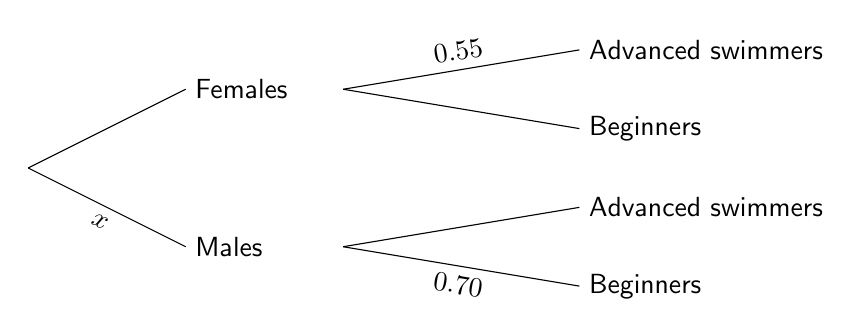
\begin{tikzpicture}
			\draw (0,0) --(2,1) node[right]{Females};
			
			\draw         (4,1) --node[midway,rotate=atan(1/6),above]{$0.55$} (7,1.5) node[right]{Advanced swimmers};
			
			\draw         (4,1) -- (7,0.5) node[right]{Beginners};
			
			\draw (0,0) --node[midway,rotate=-atan(1/2),below]{$x$}(2,-1) node[right]{Males};
			
			\draw         (4,-1) -- (7,-0.5) node[right]{Advanced swimmers};
			
			\draw         (4,-1) --node[midway,rotate=-atan(1/6),below]{$0.70$} (7,-1.5) node[right]{Beginners};
			
		\end{tikzpicture}
	\end{figure*}
	
	For a randomly chosen member, the probability of being an Advanced swimmer is the same as the
	probability of being a Beginner. 
	
	\begin{enumerate}[label=(\roman*)]
		\item Find $x$ \hfill [3]
		\item Given that a randomly chosen member is an Advanced swimmer, find the probability that the
		member is male. \hfill [3]
	\end{enumerate}
	
	
%%%%%%%%%%%%%%%%%%%%%%%%%%%%%%%%%%	
%%%%%%%%%%%%%%%%%%%%%%%%%%%%%%%%%%	
%%%%%%%%%%%%%%%%%%%%%%%%%%%%%%%%%%	
%%%%    Q2 s19_qp_62  q1     %%%	
%%%%%%%%%%%%%%%%%%%%%%%%%%%%%%%%%%	
%%%%%%%%%%%%%%%%%%%%%%%%%%%%%%%%%%	
%%%%%%%%%%%%%%%%%%%%%%%%%%%%%%%%%%		

\item	Two ordinary fair dice are thrown and the numbers obtained are noted. Event $S$ is 'The sum of the numbers is even'. Event $T$ is 'The sum of the numbers is either less than $6$ or a multiple of $4$ or both'. Showing your working, determine whether the events $S$ and $T$ are independent. \hfill  [4]
	
	
	
%%%%%%%%%%%%%%%%%%%%%%%%%%%%%%%%%%	
%%%%%%%%%%%%%%%%%%%%%%%%%%%%%%%%%%	
%%%%%%%%%%%%%%%%%%%%%%%%%%%%%%%%%%	
%%%%    Q3 w17_qp_61  q5     %%%	
%%%%%%%%%%%%%%%%%%%%%%%%%%%%%%%%%%	
%%%%%%%%%%%%%%%%%%%%%%%%%%%%%%%%%%	
%%%%%%%%%%%%%%%%%%%%%%%%%%%%%%%%%%		

\item 	Over a period of time Julian finds that on long-distance flights he flies economy class on $82\%$ of flights. On the rest of the flights he flies first class. When he flies economy class, the probability that he gets a good night's sleep is $x$. When he flies first class, the probability that he gets a good night's
sleep is $0.9$.

\begin{enumerate}[label=(\roman*)]
	\item Draw a fully labelled tree diagram to illustrate this situation. \hfill[2]
\end{enumerate}

The probability that Julian gets a good night's sleep on a randomly chosen flight is $0.285$.

\begin{enumerate}[resume,label=(\roman*)]
	\item Find the value of $x$. \hfill [2]
	\item Given that on a particular flight Julian does not get a good night's sleep, find the probability that he is flying economy class. \hfill [3]
\end{enumerate}
	

%%%%%%%%%%%%%%%%%%%%%%%%%%%%%%%%%%	
%%%%%%%%%%%%%%%%%%%%%%%%%%%%%%%%%%	
%%%%%%%%%%%%%%%%%%%%%%%%%%%%%%%%%%	
%%%%    Q4 w18_qp_61  q7     %%%	
%%%%%%%%%%%%%%%%%%%%%%%%%%%%%%%%%%	
%%%%%%%%%%%%%%%%%%%%%%%%%%%%%%%%%%	
%%%%%%%%%%%%%%%%%%%%%%%%%%%%%%%%%%		

\item In a group of students, the numbers of boys and girls studying Art, Music and Drama are given in the following table. Each of these $160$ students is studying exactly one of these subjects.

\begin{table}[!htpb]
	\centering
	\begin{tabular}{l|c|c|c|}
		\cline{2-4}
		& Art & Music & Drama \\ \hline
		\multicolumn{1}{|l|}{Boys}  & 24  & 40    & 32    \\ \hline
		\multicolumn{1}{|l|}{Girls} & 15  & 12    & 37    \\ \hline
	\end{tabular}
\end{table}

\begin{enumerate}[label=(\roman*)]
	\item Find the probability that a randomly chosen student is studying Music. \hfill[1]
	\item Determine whether the events 'a randomly chosen student is a boy' and 'a randomly chosen
	student is studying Music' are independent, justifying your answer. \hfill [2]
	\item Find the probability that a randomly chosen student is not studying Drama, given that the student	is a girl. \hfill [2]
	\item Three students are chosen at random. Find the probability that exactly $1$ is studying Music and 	exactly $2$ are boys. \hfill  [5]
\end{enumerate}



%%%%%%%%%%%%%%%%%%%%%%%%%%%%%%%%%%	
%%%%%%%%%%%%%%%%%%%%%%%%%%%%%%%%%%	
%%%%%%%%%%%%%%%%%%%%%%%%%%%%%%%%%%	
%%%%    Q5 w18_qp_63  q3    %%%	
%%%%%%%%%%%%%%%%%%%%%%%%%%%%%%%%%%	
%%%%%%%%%%%%%%%%%%%%%%%%%%%%%%%%%%	
%%%%%%%%%%%%%%%%%%%%%%%%%%%%%%%%%%		

\item A box contains $3$ red balls and $5$ blue balls. One ball is taken at random from the box and not replaced. A yellow ball is then put into the box. A second ball is now taken at random from the box.

\begin{enumerate}[label=(\roman*)]
	\item  Complete the tree diagram to show all the outcomes and the probability for each branch. \hfill[2]
	
	\begin{figure*}[!htpb]
		\centering
		\begin{tikzpicture}
			\draw (0,0) --(2,1.5);
			
			\draw         (4,1.5) -- (7,2.5);
			
			\draw         (4,1.5) -- (7,1.5);
			\draw         (4,1.5) -- (7,0.5);
			
		\draw (0,0) --(2,-1.5);
		
		\draw         (4,-1.5) -- (7,-2.5);
		
		\draw         (4,-1.5) -- (7,-1.5);
		\draw         (4,-1.5) -- (7,-0.5);
		
		\node at (3,3.5) {First ball};
		\node at (8,3.5) {Second ball};
			
		\end{tikzpicture}
	\end{figure*}



\item  Find the probability that the two balls taken are the same colour.  \hfill[2]

\item  Find the probability that the first ball taken is red, given that the second ball taken is blue. \hfill [3]




\end{enumerate}


%%%%%%%%%%%%%%%%%%%%%%%%%%%%%%%%%%	
%%%%%%%%%%%%%%%%%%%%%%%%%%%%%%%%%%	
%%%%%%%%%%%%%%%%%%%%%%%%%%%%%%%%%%	
%%%%    Q6 w16_qp_61  q6    %%%	
%%%%%%%%%%%%%%%%%%%%%%%%%%%%%%%%%%	
%%%%%%%%%%%%%%%%%%%%%%%%%%%%%%%%%%	
%%%%%%%%%%%%%%%%%%%%%%%%%%%%%%%%%%		

\item Deeti has $3$ red pens and $1$ blue pen in her left pocket and $3$ red pens and $1$ blue pen in her right pocket. 'Operation $T$' consists of Deeti taking one pen at random from her left pocket and placing it in her right pocket, then taking one pen at random from her right pocket and placing it in her left pocket.

\begin{enumerate}[label=(\roman*)]
	\item Find the probability that, when Deeti carries out operation $T$, she takes a blue pen from her left pocket and then a blue pen from her right pocket. \hfill[2]
\end{enumerate}

The random variable $X$ is the number of blue pens in Deeti's left pocket after carrying out operation $T$.

\begin{enumerate}[resume,label=(\roman*)]
	\item Find P($X$) = $1$. \hfill[3]
	\item Given that the pen taken from Deeti's right pocket is blue, find the probability that the pen taken
	from Deeti's left pocket is blue. \hfill [4]
\end{enumerate}


%%%%%%%%%%%%%%%%%%%%%%%%%%%%%%%%%%	
%%%%%%%%%%%%%%%%%%%%%%%%%%%%%%%%%%	
%%%%%%%%%%%%%%%%%%%%%%%%%%%%%%%%%%	
%%%%    Q7 m16_qp_62  q3    %%%	
%%%%%%%%%%%%%%%%%%%%%%%%%%%%%%%%%%	
%%%%%%%%%%%%%%%%%%%%%%%%%%%%%%%%%%	
%%%%%%%%%%%%%%%%%%%%%%%%%%%%%%%%%%		

\item A fair eight-sided die has faces marked $1$, $2$, $3$, $4$, $5$, $6$, $7$, $8$. The score when the die is thrown is the number on the face the die lands on. The die is thrown twice.

\begin{itemize}
	\setlength\itemsep{0.5em}
	\item Event $R$ is 'one of the scores is exactly $3$ greater than the other score'.
	\item Event $S$ is 'the product of the scores is more than $19$'.
\end{itemize}

\begin{enumerate}[label=(\roman*)]
	\item Find the probability of $R$. \hfill[2]
	\item Find the probability of $S$. \hfill[2]
	\item Determine whether events $R$ and $S$ are independent. Justify your answer. \hfill[3]
\end{enumerate}

%%%%%%%%%%%%%%%%%%%%%%%%%%%%%%%%%%	
%%%%%%%%%%%%%%%%%%%%%%%%%%%%%%%%%%	
%%%%%%%%%%%%%%%%%%%%%%%%%%%%%%%%%%	
%%%%    Q8 s15_qp_61  q3    %%%	
%%%%%%%%%%%%%%%%%%%%%%%%%%%%%%%%%%	
%%%%%%%%%%%%%%%%%%%%%%%%%%%%%%%%%%	
%%%%%%%%%%%%%%%%%%%%%%%%%%%%%%%%%%		

\item Jason throws two fair dice, each with faces numbered $1$ to $6$. Event A is 'one of the numbers obtained
is divisible by $3$ and the other number is not divisible by $3$'. Event $B$ is 'the product of the two
numbers obtained is even'.

\begin{enumerate}[label=(\roman*)]
	\item Determine whether events $A$ and $B$ are independent, showing your working.  \hfill[5]
	\item Are events $A$ and $B$ mutually exclusive? Justify your answer. \hfill[1]
\end{enumerate}

\newpage 
%%%%%%%%%%%%%%%%%%%%%%%%%%%%%%%%%%	
%%%%%%%%%%%%%%%%%%%%%%%%%%%%%%%%%%	
%%%%%%%%%%%%%%%%%%%%%%%%%%%%%%%%%%	
%%%%    Q9 s15_qp_63  q2    %%%	
%%%%%%%%%%%%%%%%%%%%%%%%%%%%%%%%%%	 
%%%%%%%%%%%%%%%%%%%%%%%%%%%%%%%%%%	
%%%%%%%%%%%%%%%%%%%%%%%%%%%%%%%%%%		

\item	When Joanna cooks, the probability that the meal is served on time is $\frac{1}{5}$. The probability that the
kitchen is left in a mess is $\frac{3}{5}$. The probability that the meal is not served on time and the kitchen is not
left in a mess is $\frac{3}{10}$. Some of this information is shown in the following table.


\medskip

\begin{table}[!htpb]
	\centering
	\begin{tabular}{l|c|c|c|}
		\cline{2-4}
		& Kitchen left in a mess & Kitchen left not in a mess & Total \\ \hline
		\multicolumn{1}{|l|}{Meal served on time}     &                        &                            &   $\frac{1}{5}$    \\ \hline
		\multicolumn{1}{|l|}{Meal not served on time} &                        &                  $\frac{3}{10}$          &       \\ \hline
		\multicolumn{1}{|l|}{Total}                   &                        &                            & 1     \\ \hline
	\end{tabular}
\end{table}

\begin{enumerate}[label=(\roman*)]
	\item Copy and complete the table. \hfill[3]
	\item Given that the kitchen is left in a mess, find the probability that the meal is not served on time. 
	
	
	\,\quad 
	\hfill 
	[2]
\end{enumerate}


%%%%%%%%%%%%%%%%%%%%%%%%%%%%%%%%%%	
%%%%%%%%%%%%%%%%%%%%%%%%%%%%%%%%%%	
%%%%%%%%%%%%%%%%%%%%%%%%%%%%%%%%%%	
%%%%    Q10 s14_qp_63  q6    %%%	
%%%%%%%%%%%%%%%%%%%%%%%%%%%%%%%%%%	
%%%%%%%%%%%%%%%%%%%%%%%%%%%%%%%%%%	
%%%%%%%%%%%%%%%%%%%%%%%%%%%%%%%%%%		

\item Tom and Ben play a game repeatedly. The probability that Tom wins any game is $0.3$. Each game is
won by either Tom or Ben. Tom and Ben stop playing when one of them (to be called the champion)
has won two games.

\begin{enumerate}[label=(\roman*)]
	\item Find the probability that Ben becomes the champion after playing exactly $2$ games. \hfill [1]
	
	\item Find the probability that Ben becomes the champion.  \hfill[3]
	\item Given that Tom becomes the champion, find the probability that he won the $2$nd game. \hfill[4]
\end{enumerate}



	
\end{enumerate}

	

	
	
	
	
	




	\newpage
\section{Discrete random variables}
%%%%%%%%%%%%%%%%%%%%%%%%%%%%%%%%%%%%%%%%%%%%%
%%%%%%%%%%%%%%%%%%%%%%%%%%%%%%%%%%%%%%%%%%%%%
%%%%%%%%%%%%%%%%%%%%%%%%%%%%%%%%%%%%%%%%%%%%%
%%%%%%%%%%%%%%%%%%%%%%%%%%%%%%%%%%%%%%%%%%%%%
%% 4.1 Introduction %%%
%%%%%%%%%%%%%%%%%%%%%%%%%%%%%%%%%%%%%%%%%%%%%
%%%%%%%%%%%%%%%%%%%%%%%%%%%%%%%%%%%%%%%%%%%%%
%%%%%%%%%%%%%%%%%%%%%%%%%%%%%%%%%%%%%%%%%%%%%
%%%%%%%%%%%%%%%%%%%%%%%%%%%%%%%%%%%%%%%%%%%%%
%\setlength\itemsep{0.5em}

\subsection{Introduction}

A discrete random variables is a variable which can take individual values each with a given $\underline{\hspace{2cm}}$.

\medskip

Notation:


\begin{itemize}
	\setlength\itemsep{0.5em}
	\item Random variables are denoted by \underline{\hspace{3cm}}
	\item Particular values of variables are denoted by \underline{\hspace{3cm}}
	\item The probability that the variable $X$ takes a particular value  is written  \underline{\hspace{3cm}}
\end{itemize}


Probability distributions:z
\medskip

A list of all possible values of the discrete random variable $X$, together with their associated probabilities.

\begin{table}[!htpb]
	\centering
	\begin{tabular}{|l|c|c|c|c|c|}
		\hline
		$x $     & $x_1$ & $x_2$ & $x_3$ & \ldots & $x_n$ \\ \hline
		P($X=x$) & $p_1$ & $p_2$ & $p_3$ & \ldots & $p_n$ \\ \hline
	\end{tabular}
\end{table}
	
Sum of probabilities:

\[
\text{P}(X=x_1) + \text{P}(X=x_2) + \text{P}(X=x_3) + \cdots + \text{P}(X=x_n) =1
\]	

Alternatively you can write 

\[
p_1 + p_2 +\cdots + p_n =1
\]


\exercise   %%%%% Exercise 20

\begin{enumerate}
	\item Emma is playing a game with a blased  five-sided spinner marked with the numbers $1$,$2$, $3$, $4$ and $5$.
	
	When she spins the spinner, her score, $X$, is the number on which the spinner lands. The probability distribution of $X$ is shown in the table. 
	
	\begin{table}[!htpb]
		\centering
		\begin{tabular}{|l|c|c|c|c|c|}
			\hline
			$x $     & $1$ & $2$ & $3$ & $4$ & $5$ \\ \hline
			P($X=x$) & $0.15$ & $0.24$ & $a$ & $0.25$ & $0.19$ \\ \hline
		\end{tabular}
	\end{table}
	
	\begin{enumerate}
		\item Find the value of $a$.
		\item Find the probability that the score is at least $4$.
		\item Find the probability that the score is less than  $5$.
		\item Find P($2<x\leqslant 4$).
		\item Write down the most likely score.
	\end{enumerate}
	
	
	\item Lancelot decides to replace the two used batteries in his torch with new ones. Unfortunately, when he takes them out, he mixes them up with three new batteries. All five batteries are identical in appearance.
	
	Lancelot selects two of the batteries at random. Draw up a probability distribution table for $X$,  the number of \textbf{new} batteries that Lancelot selects.
	
	
	\item A vegetable basket contains $12$ peppers, of which $3$ are red, $3$ are green and $5$ are yellow. Three peppers are taken at random, without replacement, from the basket.
	
	\begin{enumerate}
		\item Find the probability that the three peppers are all different colours.
		\item Show that the probability that exactly $2$ of the peppers taken are green is $\frac{12}{55}$.
		\item The number of \textbf{green} peppers taken is denoted by the discrete random variable $X$. Draw up a probability distribution table for $X$.
	\end{enumerate}
	
	
	
	\item In a probability distribution the random variable $X$ takes the value $x$ with probability $kx$, where $x$ takes the value $5$, $10$, $15$, $20$ and $25$ only.
	
	Draw up a probability distribution for $X$, in terms of $k$, and find the value of $k$.
	
	
	\item Sherry has two fair tetrahedral (four-sided) dice. The faces on each die are labelled $1$, $2$, $3$ and $4$. One die is red and the other is blue. Sherry throws  each die once. The random variable $X$ is the sum of the numbers on which the dice land.
	
	\begin{enumerate}
		\item Find the probability that $X=4$.
		\item Draw up a probability distribution table for $X$.
		\item Given that $X=6$, find the probability that the red die landed on $2$.
	\end{enumerate} 
	
	
	\item Laura is playing a game in which he tries to throw tennis balls  into a bucket. The probability that the tennis ball lands in the bucket is $0.4$ for each attempt.
	
	Laura has three attempts.
	
	\begin{enumerate}
		\item By drawing a tree diagram, or otherwise, show that the probability that exactly one tennis ball lands in the bucket is $0.432$.
		
		\item Draw up a probability distribution table for $X$, the number of tennis balls that land in the bucket.
	\end{enumerate}
	
	
	Laura wins a prize if at least two tennis balls  land in the bucket.
	
	\begin{enumerate}[resume]
		\item What is the probability that he wins a prize.
	\end{enumerate}
	
	
\end{enumerate}
	
\newpage	
%%%%%%%%%%%%%%%%%%%%%%%%%%%%%%%%%%%%%%%%%%%%%
%%%%%%%%%%%%%%%%%%%%%%%%%%%%%%%%%%%%%%%%%%%%%
%%%%%%%%%%%%%%%%%%%%%%%%%%%%%%%%%%%%%%%%%%%%%
%%%%%%%%%%%%%%%%%%%%%%%%%%%%%%%%%%%%%%%%%%%%%
%% 4.2 Expectation %%%
%%%%%%%%%%%%%%%%%%%%%%%%%%%%%%%%%%%%%%%%%%%%%
%%%%%%%%%%%%%%%%%%%%%%%%%%%%%%%%%%%%%%%%%%%%%
%%%%%%%%%%%%%%%%%%%%%%%%%%%%%%%%%%%%%%%%%%%%%
%%%%%%%%%%%%%%%%%%%%%%%%%%%%%%%%%%%%%%%%%%%%%
%\setlength\itemsep{0.5em}

\subsection{E($X$), the expectation of $X$}	




	\input{Sections/Binomial distribution}
	
    
\end{document}